\documentclass[a4paper,ngerman,naustrian,DIV=12,BCOR=1cm]{scrbook}
\usepackage[T1]{fontenc}
\usepackage[utf8]{inputenc}
\usepackage{fancyhdr}
\pagestyle{fancy}
\setcounter{secnumdepth}{3}
\usepackage{babel}
\usepackage{textcomp}
\usepackage{url}
\usepackage{makeidx}
\usepackage{float}
\usepackage{wrapfig}
\makeindex
\usepackage{graphicx}
\usepackage{epstopdf}
\PassOptionsToPackage{normalem}{ulem}
\usepackage{ulem}
\usepackage{needspace}
\usepackage[unicode=true,
 bookmarks=true,bookmarksnumbered=false,bookmarksopen=false,
 breaklinks=true,pdfborder={0 0 0},backref=false,colorlinks=false]
 {hyperref}
\hypersetup{pdftitle={sblit},
 pdfauthor={Martin Exner, Andreas Novak, Nikola Szucsich},
 pdfsubject={Diplomarbeit},
 pdfkeywords={Diplomarbeit}}

\makeatletter

%%%%%%%%%%%%%%%%%%%%%%%%%%%%%% LyX specific LaTeX commands.
\pdfpageheight\paperheight
\pdfpagewidth\paperwidth

%% Because html converters don't know tabularnewline
\providecommand{\tabularnewline}{\\}

%%%%%%%%%%%%%%%%%%%%%%%%%%%%%% Textclass specific LaTeX commands.
\newcommand{\strong}[1]{\textbf{#1}}
\newcommand{\code}[1]{\texttt{#1}}

%%%%%%%%%%%%%%%%%%%%%%%%%%%%%% User specified LaTeX commands.
%%%%%%%%%%%%
% Latex-Vorspann
\usepackage{lastpage}
\usepackage{listings}
\usepackage{blindtext}

%% geht nicht mit jeder Latex Variante, gibt aber ein schöneres Layout
\usepackage{microtype}

%% Aufzählungen nicht so weit einrücken
\usepackage{enumitem}
%\setitemize{leftmargin=*}

% Serifenschrift für Überschriften
\addtokomafont{disposition}{\rmfamily}

% Serifenschrift für Description-Lists
\setlist[description]{font=\rmfamily}

%\usepackage{caladea}
%\usepackage[T1]{fontenc}
\usepackage{lmodern}

%% für pandoc
%% maximale Breite der Bilder
\setkeys{Gin}{width=0.90\linewidth,keepaspectratio}

\makeatother

\usepackage{listings}
\addto\captionsnaustrian{\renewcommand{\lstlistingname}{Listing}}
\addto\captionsngerman{\renewcommand{\lstlistingname}{Listing}}
\renewcommand{\lstlistingname}{Listing}

% to insert a space after use of an argument-less command depending on what follows (\xspace)
\usepackage{xspace}

% to use with java syntax highlighting
\usepackage{color}

% to draw packet structures
\usepackage{bytefield}

% to include pages from PDF files
\usepackage{pdfpages}

% to place tables exactly here
\usepackage{float}
\restylefloat{table}

% global definitions

\newcommand{\kap}[1]{(\textbf{deprecated}) \link{#1}} % TODO remove

\newcommand{\labellinkt}[1]{\ref{#1} \nameref{#1}}
\newcommand{\labellink}[1]{\hyperref[#1]{\labellinkt{#1}}}
\newcommand{\pagelinkt}[1]{Seite~\pageref{#1}}
\newcommand{\pagelink}[1]{\hyperref[#1]{\pagelinkt{#1}}}
\newcommand{\linkt}[1]{\labellinkt{#1}, \pagelinkt{#1}}
\newcommand{\link}[1]{\hyperref[#1]{\linkt{#1}}}
\newcommand{\siehet}[1]{siehe~\linkt{#1}}
\newcommand{\siehe}[1]{\hyperref[#1]{\siehet{#1}}}
\newcommand{\referenz}[1]{\hyperref[#1]{(\siehet{#1})}}
\newcommand{\abbildung}[1]{(siehe \figurelinkt{dcl-sblit-#1-bytefield})}
\newcommand{\figurelinkt}[1]{Abbildung~\ref{#1}, \nameref{#1}}
\newcommand{\figurelink}[1]{\hyperref[#1]{\figurelinkt{#1}}}
\newcommand{\figurelinkpt}[1]{Abbildung~\ref{#1}, \nameref{#1}, \pagelinkt{#1}}
\newcommand{\figurelinkp}[1]{\hyperref[#1]{\figurelinkpt{#1}}}

\newcommand{\codeline}[1]{\sloppy{\mbox{\code{#1}}}}

\newcommand{\tags}[2]{\hspace{0in}#2}

\newcommand{\sblit}{sblit\xspace}
\newcommand{\sblitg}{\sblit}

\newcommand{\addrkeybits}{2048\xspace}
\newcommand{\addrkeybytes}{256\xspace}

\newcommand{\javaarg}{Argument\xspace}
\newcommand{\javainstvar}{Instanzvariable\xspace}

\newcommand{\cnettype}{org.dclayer.circle}
\newcommand{\cnetattr}{sha1/20}
\newcommand{\cnetid}{\cnettype{} \cnetattr{}}

\newcommand{\msg}[1]{#1 Message}
\newcommand{\msgpl}[1]{#1 Messages}

\newcommand{\comp}[1]{#1 Component}

\newcommand{\isprotomsgtype}{Message Type}
\newcommand{\isprotomsgdata}{Message Data}

\newcommand{\flexnumfield}{\glslink{fnumc}{FlexNum, 1 -- 9 Bytes}}
\newcommand{\netpktfield}{\glslink{netpkt}{NetworkPacket, $N$ Bytes}}

\newcommand{\descriptionitem}[1]{\item[{#1}] \hfill \nopagebreak \\}
\newcommand{\datei}[1]{\textit{#1}}

\newcommand{\const}[1]{\code{#1}}

% shamelessly stolen from http://tex.stackexchange.com/a/35943 and modified
\newcommand{\namesigdate}[2][8cm]{
    \begin{tabular}{@{}p{#1}@{}}
        \\
        \\
        \\
        \\
        \hrule \\
        \small{#2}
    \end{tabular}
}


\newcommand{\isgeneralbytefield}{\begin{figure}[tbh]\begin{centering}\begin{bytefield}[bitwidth=3.0em]{8} \\ \bitheader{0-7} \\ \wordbox[lrt]{2}{\isprotomsgtype \\ \flexnumfield} \\ 
\skippedwords \\ 
\wordbox[lr]{1}{} \\ 
\wordbox[lrt]{2}{\isprotomsgdata \\ $N$ Bytes} \\ 
\skippedwords \\ 
\wordbox[lrb]{1}{}\end{bytefield}\par\end{centering}\protect\caption{\gls*{isproto} -- Genereller Messageaufbau}\end{figure}}

\newcommand{\isprotoversionbytefield}{\begin{figure}[tbh]\begin{centering}\begin{bytefield}[bitwidth=3.0em]{8} \\ 
\bitheader{0-7} \\ 
\begin{rightwordgroup}{Message Type}
\wordbox[lrt]{1}{\code{0}}

\end{rightwordgroup}
 \\ 
\wordbox[lrt]{2}{Version \\ \flexnumfield} \\ 
\skippedwords \\ 
\wordbox[lrb]{1}{}
\end{bytefield}\par\end{centering}
\protect\caption{\gls*{isproto} -- \isprotoversion-Message}
\end{figure}}

\newcommand{\isprotollareqbytefield}{\begin{figure}[tbh]\begin{centering}\begin{bytefield}[bitwidth=3.0em]{8} \\ 
\bitheader{0-7} \\ 
\begin{rightwordgroup}{Message Type}
\wordbox[lrt]{1}{\code{1}}

\end{rightwordgroup}
 \\ 
\wordbox[lrt]{2}{Limit \\ \flexnumfield} \\ 
\skippedwords \\ 
\wordbox[lrb]{1}{}
\end{bytefield}\par\end{centering}
\protect\caption{\gls*{isproto} -- \isprotollareq-Message}
\end{figure}}

\newcommand{\isprotollarepbytefield}{\begin{figure}[H]\begin{centering}\begin{bytefield}[bitwidth=3.0em]{8} \\ 
\bitheader{0-7} \\ 
\begin{rightwordgroup}{Message Type}
\wordbox[lrt]{1}{\code{2}}

\end{rightwordgroup}
 \\ 
\begin{rightwordgroup}{LLA}
\wordbox[lrt]{2}{LLA Type \\ \flexnumfield} \\ 
\skippedwords \\ 
\wordbox[lr]{1}{}
 \\ 
\wordbox[lrt]{2}{LLA Data} \\ 
\skippedwords \\ 
\wordbox[lr]{1}{}

\end{rightwordgroup}
 \\ 
\begin{rightwordgroup}{LLA}
\wordbox[lrt]{2}{$\cdots$} \\ 
\skippedwords \\ 
\wordbox[lrb]{1}{}

\end{rightwordgroup}
\end{bytefield}\par\end{centering}
\protect\caption{\gls*{isproto} -- \isprotollarep-Message}
\end{figure}}

\newcommand{\isprototsbytefield}{\begin{figure}[tbh]\begin{centering}\begin{bytefield}[bitwidth=3.0em]{8} \\ 
\bitheader{0-7} \\ 
\begin{rightwordgroup}{Message Type}
\wordbox[lrt]{1}{\code{3}}

\end{rightwordgroup}
 \\ 
\wordbox[lrt]{2}{Address Slot \\ \flexnumfield} \\ 
\skippedwords \\ 
\wordbox[lr]{1}{}
 \\ 
\begin{rightwordgroup}{Address Key}
\wordbox[lrt]{1}{Key Type}
 \\ 
\wordbox[lrt]{2}{Key Data} \\ 
\skippedwords \\ 
\wordbox[lrb]{1}{}

\end{rightwordgroup}
\end{bytefield}\par\end{centering}
\protect\caption{\gls*{isproto} -- \isprotots-Message}
\end{figure}}

\newcommand{\isprotoccreqbytefield}{\begin{figure}[tbh]\begin{centering}\begin{bytefield}[bitwidth=3.0em]{8} \\ 
\bitheader{0-7} \\ 
\begin{rightwordgroup}{Message Type}
\wordbox[lrt]{1}{\code{4}}

\end{rightwordgroup}
 \\ 
\wordbox[lrt]{2}{Address Slot \\ \flexnumfield} \\ 
\skippedwords \\ 
\wordbox[lr]{1}{}
 \\ 
\begin{rightwordgroup}{Challenge Data}
\wordbox[lrt]{2}{Data Length \\ \flexnumfield} \\ 
\skippedwords \\ 
\wordbox[lr]{1}{}
 \\ 
\wordbox[lrt]{2}{Data} \\ 
\skippedwords \\ 
\wordbox[lrb]{1}{}

\end{rightwordgroup}
\end{bytefield}\par\end{centering}
\protect\caption{\gls*{isproto} -- \isprotoccreq-Message}
\end{figure}}


% listings

\definecolor{javastring}{rgb}{0.6,0,0} % for strings
\definecolor{javacomment}{rgb}{0.25,0.5,0.35} % comments
\definecolor{javakeyword}{rgb}{0.5,0,0.35} % keywords
\definecolor{javadoc}{rgb}{0.25,0.35,0.75} % javadoc

\newcommand{\javalisting}{\lstset{language=Java, breaklines=true, basicstyle=\ttfamily, keywordstyle=\color{javakeyword}\bfseries, stringstyle=\color{javastring}, commentstyle=\color{javacomment}, morecomment=[s][\color{javadoc}]{/**}{*/}, numbers=left, numberstyle=\tiny, stepnumber=1, numbersep=5pt, tabsize=4, showspaces=false, showstringspaces=false, frame=single}}

\newcommand{\messagestart}{\begin{figure}[p] \centering \begin{bytefield}[bitwidth=2em]{8}}
\newcommand{\messageend}[1]{\end{bytefield} \par \protect\caption{\gls{#1}} \label{#1fig} \end{figure}}


\newcommand{\listingstart}[1]{\javalisting \begin{lstlisting}[caption={#1},captionpos=b]}

%\lstset{numbers=right, numberstyle=\tiny, stepnumber=2, numbersep=5pt, showspaces=false, frame=single}


% glossaries
\usepackage[toc,acronym]{glossaries}
\makeglossaries

% DO NOT ADD ENTRIES HERE
% Add them in your *_glossary.tex file instead


\newglossaryentry{gls_udp}{
	name=User Datagram Protocol,
	description={Verbindungsloses Übertragungsprotokoll aus der Internet protocol suite \cite{wikipedia:udp}}
}

\newacronym[see={[Glossar:]{gls_udp}}]{udp}{UDP}{User Datagram Protocol\glsadd{gls_udp}}

\newglossaryentry{gls_tcp}{
	name=Transmission Control Protocol,
	description={Verbindungsorientiertes, verlässliches Übertragungsprotokoll aus der Internet protocol suite \cite{wikipedia:tcp}}
}

\newacronym[see={[Glossar:]{gls_tcp}}]{tcp}{TCP}{Transmission Control Protocol\glsadd{gls_tcp}}

\newglossaryentry{cl}{
	name=Kommunikationsschicht,
	description={Eine Schicht im netzwerktechnischen Sinne, die zur Kommunikation verwendet wird},
	see={[Siehe:]{gls_dcl}}
}

\newglossaryentry{p2pnet}{
	name=Peer-to-Peer-Netzwerk,
	plural=Peer-to-Peer-Netzwerke,
	description={Ein Kommunikationsnetzwerk, in dem die einzelnen Kommunikationspartner im Gegensatz zu einer klassischen Client-Server-Infrastruktur direkt miteinander kommunizieren}
}

\newglossaryentry{gls_dcl}{
	name=Decentralized Communication Layer,
	description={Die auf einem dezentralen \gls{p2pnet} basierende \gls{cl}, die \sblit zur Kommunikation benutzt}
}

\newacronym[see={[Glossar:]{gls_dcl}}]{dcl}{DCL}{Decentralized Communication Layer\glsadd{gls_dcl}}

\newglossaryentry{aenc}{
	name=Asymmetrisches Verschlüsselungsverfahren,
	description={Verschlüsselungsverfahren, bei dem zur Entschlüsselung einer Nachricht ein anderer Schlüssel verwendet wird, als zur Verschlüsselung verwendet wurde},
	see={[Siehe:]{rsa}}
}

\newglossaryentry{rsa}{
	name=RSA,
	description={\gls{aenc}, benannt nach und erstmals veröffentlich von Ron Rivest, Adi Shamir and Leonard Adleman \cite{wikipedia:rsa}},
	see={[Siehe:]{aenc}}
}

\newglossaryentry{gls_aes}{
	name=Advanced Encryption Standard,
	description={Standard-Verschlüsselungsverfahren für \glspl{link}},
	see={[Siehe:]{link}}
}

\newacronym[see={[Glossar:]{gls_aes}}]{aes}{AES}{Advanced Encryption Standard\glsadd{gls_aes}}

\newglossaryentry{gls_gcm}{
	name=Galois/Counter Mode,
	description={Standard-Betriebsmodus für die Verschlüsselung von \glspl{link} mit \acrshort{aes}},
}

\newacronym[see={[Glossar:]{gls_gcm}}]{gcm}{GCM}{Galois/Counter Mode\glsadd{gls_gcm}}

\newglossaryentry{hash}{
	name=Hashalgorithmus,
	plural=Hashalgorithmen,
	description={Algorithmus, der eine große Eingabemenge auf eine kleinere Zielmenge (\gls{hashval}) abbildet \cite{wikipedia:hash}}
}

\newglossaryentry{hashval}{
	name=Hashwert,
	plural=Hashwerte,
	description={Ergebnis bei Anwendung eines \gls{hash}}
}

\newglossaryentry{digestlength}{
	name=Digest Length,
	description={Die Länge der \glspl{hashval} eines \gls{hash}}
}

\newglossaryentry{sha1}{
	name=SHA-1,
	description={Im \gls{dcl} standardmäßig verwendeter \gls{hash}. SHA steht für Secure Hash Algorithm},
	see={[Siehe:]{hash}}
}

\newglossaryentry{remotekey}{
	name=Remote Key,
	description={Schlüssel, der lokal nicht bekannt ist und zu dessen besitzender Anwendung eine Verbindung besteht, über die Verschlüsselungs- und Entschlüsselungsanfragen weitergeleitet werden. Siehe \link{dcl-asproto-remotekeys}}
}

\newglossaryentry{net}{
	name=Netzwerk,
	plural=Netzwerke,
	description={Ein \gls{p2pnet} innerhalb des \gls{dcl}},
	see={[Siehe:]{cnet}}
}

\newglossaryentry{nt}{
	name=Network Type,
	plural=Network Types,
	description={Beschreibt ein \gls{net} innerhalb des \gls{dcl} samt Adresskonzept und Routingverfahren},
	see={[Siehe:]{net}}
}

\newglossaryentry{ntid}{
	name=Network Type Identifier,
	plural=Network Type Identifiers,
	description={Der eindeutige Name eines \gls{nt}},
	see={[Siehe:]{nt}}
}

\newglossaryentry{cnet}{
	name=Circle Network,
	description={Standard \gls{net} im \gls{dcl}, \gls{ntid} \code{\cnetid{}}},
	see={[Siehe:]{net}}
}

\newglossaryentry{cnt}{
	name=CircleNetworkType,
	description={Im Quellcode von \gls{dcl} definierte Klasse zur Darstellung des \gls{nt} des \gls{cnet}},
	see={[Siehe:]{nt}}
}

\newglossaryentry{netint}{
	name=Netzwerkintegration,
	description={Das Aufbauen von Verbindungen mit anderen \glspl{service}, um optimal in das Routing eines \glslink{net}{Netzwerks} eingebunden zu sein}
}

\newglossaryentry{service}{
	name=DCL-Service,
	description={Ein Teilnehmer des \gls{dcl}. Kann mehrere Adressen in mehreren unterschiedlichen \glslink{net}{Netzwerken} hosten}, % TODO
	see={[Siehe:]{dcl}}
}

\newglossaryentry{endp}{
	name=Endpunkt,
	plural=Endpunkte,
	description={Eine auf dem lokalen bzw. einem direkt verbundenen \gls{service} gehostete Adresse in einem bestimmten \gls{net}},
	see={[Siehe:]{Nexthops}}
}

\newglossaryentry{asendp}{
	name=Network Endpoint,
	description={Eine Kombination aus einer auf einer \gls{asconn} bekanntgegebenen Adresse und einem \gls{net}, dem die Anwendung mit dieser Adresse beigetreten ist}
}

\newglossaryentry{isproto}{
	name=Interservice-Protokoll,
	description={Das zur Kommunikation zwischen zwei direkt verbundenen \glspl{service} verwendete Protokoll}
}

\newglossaryentry{link}{
	name=Link,
	description={Verlässlicher und verschlüsselter Übertragungskanal basierend auf \acrshort{udp}. Basis für \glspl{isch}. Siehe \link{dcl-link}}
}

\newglossaryentry{channel}{
	name=Channel,
	description={Getrennter Datenkanal eines \glslink{link}{Links}. Siehe \link{dcl-link-channels}}
}

\newglossaryentry{mgmtch}{
	name=Management Channel,
	description={\Gls{channel} eines \glslink{link}{Links}, der zur Übertragung von Nachrichten zur Verwaltung des \glslink{link}{Links} genutzt wird},
	see={[Siehe:]{channel}}
}

\newglossaryentry{channelid}{
	name=Channel Identifier,
	description={Zahl zur eindeutigen Identifizierung eines \glslink{channel}{Channels} auf einem \gls{link}}
}

\newglossaryentry{dataid}{
	name=Data Identifier,
	description={Fortlaufende Zahl zur eindeutigen Identifizierung eines über einen \gls{channel} eines \glslink{link}{Links} übertragenen Datenblocks und zur Angabe der Reihenfolge dieses Datenblocks im Datenstrom des \glslink{channel}{Channels}}
}

\newglossaryentry{chblockstatrep}{
	name=Channel Block Status Report,
	description={Statusinformation über die empfangenen \glspl{dataid} eines \glslink{channel}{Channels}, anhand derer fehlende Pakete erkannt und erneut übertragen werden können},
	see={[Siehe:]{channel}}
}

\newglossaryentry{fcnt}{
	name=Flusskontrolle,
	description={Einschränkung der über einen Kommunikationskanal übertragenen Menge an Daten zur Vermeidung von Verstopfung}
}

\newglossaryentry{protoid}{
	name=Protocol Identifier,
	description={Eindeutige Kennung des Protokolls, über das auf einem \gls{channel} eines \glslink{link}{Links} kommuniziert wird}
}

\newglossaryentry{mcp}{
	name=Management Channel Protocol,
	description={Protokoll zur Verwaltung eines \glslink{link}{Links}},
	see={[Siehe:]{gls_bmcp}}
}

\newglossaryentry{gls_bmcp}{
	name=Basic Management Channel Protocol,
	description={Standardmäßig verwendetes \gls{mcp} zur Verwaltung von \glspl{link}. Siehe \link{dcl-link-bmcp}}
}

\newacronym[see={[Glossar:]{gls_bmcp}}]{bmcp}{BMCP}{Basic Management Channel Protocol\glsadd{gls_bmcp}}

\newglossaryentry{cinitmethod}{
	name=Crypto Initialization Method,
	description={Art der Verschlüsselung eines mit \acrshort{bmcp} verwalteten \glslink{link}{Links} und Methode zur Initialisierung dieser Verschlüsselung},
	see={[Siehe:]{gls_bmcp}}
}

\newglossaryentry{cimid}{
	name=Crypto Initialization Method Identifier,
	description={Zahl zur eindeutigen Kennung einer \gls{cinitmethod}},
	see={[Siehe:]{cinitmethod}}
}

\newglossaryentry{asproto}{
	name=Application-to-Service-Protokoll,
	description={Das zur Kommunikation zwischen einer Anwendung und einem \gls{service} verwendete Protokoll}
}

\newglossaryentry{asconn}{
	name=Application-to-Service-Verbindung,
	plural=Application-to-Service-Verbindungen,
	description={Verbindung über \acrshort{tcp} zwischen einer Anwendung und einem \gls{service}, auf der mittels \gls{asproto} kommuniziert wird}
}

\newglossaryentry{appch}{
	name=Application Channel,
	description={Ein verlässlicher Übertragungskanal zur Kommunikation zwischen zwei Instanzen einer auf dem \gls{dcl} aufbauenden Anwendung}
}

\newglossaryentry{cchlg}{
	name=Crypto Challenge,
	description={Anforderung, mit dem einem bekannten öffentlichen Schlüssel zugehörigen privaten Schlüssel Daten zu signieren, um so den Besitz des gesamten Schlüsselpaars zu beweisen}
}

\newglossaryentry{pktc}{
	name=Packet Component,
	description={Teil einer Message, beispielsweise Ganzzahl oder String. Siehe \link{dcl-packetcomponents}}
}

\newglossaryentry{fnumc}{
	name=FlexNum-Component,
	description={\gls{pktc} zur Übertragung einer bis zu 64 Bits großen Ganzzahl. Siehe \link{dcl-packetcomponents-flexnum}}
}

\newglossaryentry{gls_lla}{
	name=Lower Level Address,
	plural=Lower Level Addresses,
	description={Die Adresse eines \gls{service} auf der Netzwerkschicht unter \gls{dcl}, de facto die IP-Adresse und Port, unter der ein \gls{service} erreichbar ist}
}

\newacronym[plural={LLAs}, longplural={Lower Level Addresses}, see={[Glossar:]{gls_lla}}]{lla}{LLA}{Lower Level Address\glsadd{gls_lla}}

\newglossaryentry{netpkt}{
	name=Network Packet,
	description={Geroutete Nachricht innerhalb eines \glslink{net}{Netzwerks}}
}

\newglossaryentry{keyc}{
	name=Key-Component,
	description={Basis für \glspl{pktc} zur Übertragung von Schlüsseldaten}
}

\newglossaryentry{actid}{
	name=Action Identifier,
	description={String, der in Anfragen übertragen wird und Auskunft über den Grund dieser Anfrage geben soll}
}

\newglossaryentry{addrslot}{
	name=Address Slot,
	description={Zahl zur Referenzierung von auf einem \gls{service} gehosteten Adressen}
}

\newglossaryentry{netslot}{
	name=Network Slot,
	description={Zahl zur Referenzierung von \glspl{net}, denen ein \gls{service} auf einem \gls{isch} mit einer oder mehreren Adressen beigetreten ist}
}

\newglossaryentry{appchslot}{
	name=Application Channel Slot,
	description={Zahl zur Referenzierung von \glspl{appch} auf \glspl{isch}}
}

\newglossaryentry{endpslot}{
	name=Network Endpoint Slot,
	description={Zahl zur Referenzierung von \glspl{asendp} auf \glspl{asconn}}
}

\newglossaryentry{isch}{
	name=Interservice Channel,
	description={Verbindung zwischen zwei \glspl{service}, innerhalb der mit dem \gls{isproto} kommuniziert wird}
}

\newglossaryentry{connbase}{
	name=Connection Base,
	description={Berechtigungslevel für einen \gls{addrslot} eines \gls{isch}} % TODO
}

% DCL source classes

\newglossaryentry{Data}{
	name=Data,
	description={Im Quellcode von \gls{dcl} definierte Klasse zur Speicherung von Binärdaten}
}

\newglossaryentry{Hash}{
	name=Hash,
	description={Im Quellcode von \gls{dcl} definierte Klasse zur Anwendung von \glspl{hash} auf \gls{Data}-Objekte}
}

\newglossaryentry{Address}{
	name=Address,
	description={Im Quellcode von \gls{dcl} definierte Klasse zur Speicherung von öffentlichen Schlüsseln anderer Teilnehmer}
}

\newglossaryentry{Nexthops}{
	name=Nexthops,
	description={Im Quellcode von \gls{dcl} definierte Klasse zur Speicherung von verbundenen \glslink{endp}{Endpunkten} in der Form von \gls{ForwardDestination}-Objekten}
}

\newglossaryentry{ForwardDestination}{
	name=ForwardDestination,
	description={Im Quellcode von \gls{dcl} definierte Klasse zur Speicherung eines verbundenen \glslink{endp}{Endpunkts},
			an den eine Nachricht weitergeleitet werden kann, inklusive dessen \gls{Address}- und
			\gls{InterserviceChannel}-Objekten},
	see={[Siehe:]{endp}}
}

\newglossaryentry{InterserviceChannel}{
	name=InterserviceChannel,
	description={Im Quellcode von \gls{dcl} definierte Klasse zur Verwaltung einer Verbindung zwischen zwei \glspl{service}},
	see={[Siehe:]{isch}}
}

\newglossaryentry{natdev}{
	name=NAT-Gerät,
	plural=NAT-Geräte,
	description={Gerät, das \acrlong{nat} durchführt}
}

\newglossaryentry{gls_nat}{
	name=Network Address Translation,
	description={Auf \glspl{natdev} durchgeführte Übersetzung von Netzwerkadressen. Siehe \link{dcl-natt}}
}

\newacronym[see={[Glossar:]{gls_nat}}]{nat}{NAT}{Network Address Translation\glsadd{gls_nat}}

\newglossaryentry{natt}{
	name=NAT-Traversal,
	description={Umgehung von \gls{natdev}, um Peer-to-Peer-Verbindungen aufbauen zu können}
}

\newglossaryentry{nattpkt}{
	name=NAT-Traversal-Paket,
	plural=NAT-Traversal-Pakete,
	description={Paket, das im Zuge von \gls{natt} gesendet wird},
	see={[Siehe:]{natt}}
}

\newglossaryentry{nathp}{
	name=NAT Hole Punching,
	description={Verfahren zum \gls{natt}, das in der Implementierung des \gls{service} angewandt wird},
	see={[Siehe:]{natt}}
}

\newglossaryentry{ignoredata}{
	name=Ignore Data,
	plural=Ignore Data,
	description={Daten, die als Präfix für \glspl{nattpkt} verwendet werden können, die vom Empfänger ignoriert werden sollen},
	see={[Siehe:]{nattpkt}}
}

\newglossaryentry{gls_crisp}{
	name=Common Routed Interservice Protocol,
	description={Protokoll, das \gls{net}-übergreifend zur verbindungslosen Kommunikation zwischen \glspl{service} verwendet wird. Siehe \link{dcl-crisp}}
}

\newacronym[see={[Glossar:]{gls_crisp}}]{crisp}{CRISP}{Common Routed Interservice Protocol\glsadd{gls_crisp}}

\newglossaryentry{partnerdevice}{
	name=Partnergerät,
	plural=Partnergeräte,
	description={Ein Gerät eines anderen \sblit-Nutzers, mit dem eine Partnerschaft besteht}
}
\newglossaryentry{authreq}{
	name=Authenticity Request,
	description={Eine Nachricht zur Anforderung einer Challenge, um die Authentizität des Gegenübers sicherzustellen}
}
\newglossaryentry{authres}{
	name=Authenticity Response,
	description={Die Antwort auf den \gls{authreq}, um die eigene Authentizität zu beweisen}
}
\newglossaryentry{filereq}{
	name=File Request,
	description={Die Anfrage an das Gegenüber, ob eine Datei benötigt wird}
}
\newglossaryentry{fileres}{
	name=File Response,
	description={Die Antwort auf einen File Request, der eine Datei akzeptiert oder verweigert}
}
\newglossaryentry{filemsg}{
	name=File Message,
	description={Die eigentliche Übertragung einer Datei}
}
\newglossaryentry{filedel}{
	name=File Delete Message,
	description={Eine Nachricht, die dazu dient, Geräte über eine Löschung einer Datei zu informieren}
}
\newglossaryentry{filedelpart}{
	name=File Delete Message (partner),
	description={Eine Nachricht, die dazu dient, Dateien von Partnergeräten zu löschen}
}
\newglossaryentry{logfile}{
	name=Logfile,
	description={Die Datei, in der der Versionsverlauf einer Datei steht. Außerdem werden hier die Geräte, auf denen die Datei schon vorhanden ist, gelistet}
}
\newglossaryentry{refdev}{
	name=Device Refresh Message,
	description={Eine Nachricht, die eine aktualisierte Version von Partnergeräten oder eigenen Geräten enthält}
}
\newglossaryentry{partfilereq}{
	name=Partner File Request,
	description={Ein \gls{filereq} an ein Partnergerät \referenz{Partnergerät} oder von einem Partnergerät}
}
\newglossaryentry{partfileres}{
	name=Partner File Response,
	description={Ein \gls{fileres} an ein Partnergerät \referenz{Partnergerät} oder von einem Partnergerät}
}
\newglossaryentry{partfilemsg}{
	name=Partner File Message,
	description={Eine \gls{filemsg} an ein Partnergerät \referenz{Partnergerät} oder von einem Partnergerät}
}
\newglossaryentry{partfiledel}{
	name=Partner File Delete Message,
	description={Eine \gls{filedel} an ein Partnergerät \referenz{Partnergerät} oder von einem Partnergerät}
}
\newglossaryentry{watchservice}{
	name=WatchService,
	description={Eine Schnittstelle zum Filesystem, welche benachrichtigt wird, wenn sich eine Datei in einem bestimmten Ordner ändert}
}
\newglossaryentry{watchkey}{
	name=WatchKey,
	description={Ein Objekt, das vom \gls{watchservice} erstellt wird, wenn sich etwas in dem zu überwachenden Ordner ändert}
}
\newglossaryentry{symmetricKey}{
	name=Symmetrischer Schlüssel,
	description={Mithilfe dieses Schlüssels können Daten verschlüsselt und wieder entschlüsselt werden}
}
\newglossaryentry{sblit}{
	name=\sblit,
	description={Dateisynchronisationsanwendung}
}
%\newacronym[see={[Glossar:]{authreq}}]{authreq}{AuthReq}{Authenticity Request\glsadd{authreq}}


\newglossaryentry{gls_gui}{
	name=Graphical User Interface,
	description={Eine grafische Oberfläche für Benutzer, um eine Anwendung komfortabel bedienen zu können}
}

\newacronym[see={[Glossar:]{gls_gui}}]{gui}{GUI}{Graphical User Interface\glsadd{gls_gui}}

\newglossaryentry{wysiwygeditor}{
	name=What-you-see-is-what-you-get-Editor,
	description={Ein Editor, der während der Bearbeitung eines Dokuments,
	gleichzeitig das Ergebnis  grafisch darstellt. Beispiele wären der Windowbuilder bei SwingOffice-Programme
	wie Microsoft Word oder Libreoffice Writer.}
}

\newglossaryentry{m_v_c}{
	name=Model-View-Controller-Design,
	description={Ein Programmier-Pattern, bei dem Datenzugriff und Anwendungslogik von
	der grafischen Darstellung getrennt sind.}
}

\newacronym[see={[Glossar:]{m_v_c}}]{mvc}{MVC}{Model-View-Controller-Design\glsadd{m_v_c}}

\newglossaryentry{s_w_t}{
	name=Standard-Widget-Toolkit,
	description={Ein freies Framework für grafische Oberflächen, entwickelt von Eclipse.}
}

\newacronym[see={[Glossar:]{s_w_t}}]{swt}{SWT}{Standard Widget Toolkit\glsadd{s_w_t}}




\begin{document}
%%%%%%
% Weitere Einstellungen siehe Latex-Vorspann%%%%%%%%%%%%%%%%%%%%%%%%%%%%%%%%%%%%%%%%%%%%%%%%%%%%%%%%%%%%%%%%%%%%%%%%%%%%%%%%%%
% falls man die erste Zeile der Absätze nicht einrücken will
% dann sollte man aber etwas mehr Abstand zwischen den Absätzen erlauben
%%\setlength{\parindent}{0pt}
%%\setlength{\parskip}{1.5ex plus0.5ex minus0.5ex}
% Auch Fußnoten bündig ausrichten
\deffootnote[]{1em}{1em}{\textsuperscript{\thefootnotemark\ }}
% Listen etwas wenige einrücken, erfordert enumitem
\setitemize{leftmargin=*}

%%%%%%%%%%%%%%%%%%%%%%%%%%%%%%%%%%%%%%%%%%%%%%%%%%%%%%%%%%%%%%%%%%%%%%%%%%%%%%%%%%
%  Kopf und Fußzeilen -- links und rechts verschieden
\newcommand{\kopfseitenummer}{{\bfseries \thepage}}
\newcommand{\kopfkapl}{{\bfseries\leftmark}}
\newcommand{\kopfkapr}{{\bfseries\rightmark}}
\newcommand{\kopfbild}{}%
\includegraphics[width=25mm]{HTL3RLogoRGB}}
\newcommand{\kopfHTL}{Höhere Technische Bundeslehranstalt Wien 3, \\Rennweg 	Abteilung für Informationstechnologie}
\renewcommand{\chaptermark}[1]%
  {\thispagestyle{fancy}\markboth{\thechapter.\ #1}{}}%\thispagestyle{fancy}
\renewcommand{\headrulewidth}{0.2pt}
%\lhead[\fancyplain{\kopfbild}{\kopfbild}]% li aussen
%      {\fancyplain{\kopfHTL}{\kopfHTL}}% re innen
%\rhead[\kopfHTL]% li innen
%      {\kopfbild}% re aussen

%% mit kapitelautor kann man den Autor festlegen oder auf leer setzen - steht dann in der Fußzeile.
\newcommand{\kapitelautor}{}

%%%
% Alternative: am Rand (Marginale)
%\setlength{\marginparsep}{-5mm}
%\mbox{}\marginpar{\raggedleft\hspace{0pt}Autor: Hans Huber}

%% kopf links: [linke] und {rechte} Seite

\lhead[\kopfbild]{\fancyplain{}{\kopfkapl}}
\rhead[\fancyplain{}{\kopfkapr}]{\kopfbild}
\chead{}

\lfoot[\kopfseitenummer]{\kapitelautor}
\cfoot[]{}
\rfoot[\kapitelautor]{\kopfseitenummer}

%%%%%Anfang Titelseite
\pagenumbering{roman}
\title{Diplomarbeit}
\begin{titlepage}
\begin{minipage}[b]{1\columnwidth}
\parbox[b]{50mm}{
\includegraphics[width=45mm]{HTL3RLogoRGB}}
\hfill
\parbox[b]{130mm}{\footnotesize \textsc{Höhere Technische Bundeslehranstalt} Wien 3, Rennweg\\
IT \& Mechatronik\\
\\
HTL Rennweg :: Rennweg 89b\\
A-1030 Wien :: Tel +43 1 24215-10 :: Fax DW 18
}\\
\mbox{}
\end{minipage}

\vspace{1cm}


\begin{center}
\textbf{\LARGE{}Diplomarbeit}{\large{}}\\
{\large{}\vspace{15mm}
 }\textbf{\large{}sblit}\\
 \vspace{15mm}
 ausgeführt an der\\
 Höheren Abteilung für Informationstechnologie/Netzwerktechnik\\
 der Höheren Technischen Lehranstalt Wien 3 Rennweg\\
 \vspace{1cm}
 im Schuljahr 2014/2015\\
 \vspace{1cm}
 durch\\
 \vspace{0.5cm}
\textbf{\large{}Martin Exner}\\
\textbf{\large{}Andreas Novak}\\
\textbf{\large{}Nikola Szucsich}\\

\par\end{center}{\large \par}

\begin{center}
\vspace{20mm}
 \normalsize unter der Anleitung von\\
 \vspace{0.5cm}
 August Hörandl
\par\end{center}

\begin{center}
\vspace{5mm}
Wien, \today
\par\end{center}

\end{titlepage}%%%%%%%%%%%%%%%%%%%%% Ende Titelseite %%%%%%%%%%%%%%%%%%%%%%


\chapter*{Kurzfassung}

% Auf Seiten mit einem neuen Kapitel ist keine Kopfzeile -- kann man sich aber wünschen
\markboth{Kurzfassung}{}
\thispagestyle{fancy}

Diese Diplomarbeit zielt darauf ab, einen Dienst zur Synchronisation von Dateien über das Internet in der Form freier Software zu schaffen.
Zentrale Stellen wie Server sollen dabei im Sinne der Sicherheit vor Eingriffen durch Unbefugte vermieden werden.
Statt der Zwischenspeicherung von Daten auf Cloudspeicher eines herkömmlichen Anbieters werden Daten in verschlüsselten Blöcken auf den Geräten anderer, fremder Nutzer zwischengespeichert.

An die Stelle einer klassischen Client-Server-Infrastruktur tritt ein dezentrales Peer-to-Peer-Netzwerk.
Dadurch und durch die Verteilung von Daten auf Geräte anderer Teilnehmer auftretende Problemstellungen sollen im Rahmen dieser Diplomarbeit gelöst werden.
Dazu zählen dezentrale Adressierung, dezentrales Routing, Fairness von gegenseitiger Speicherfreigabe, Sicherheit und Effizienz von sowohl Kommunikation als auch Synchronisation sowie Behandlung von Synchronisationskonflikten.




\chapter*{Abstract}

% mit Kopfzeile
\markboth{Abstract}{}
\thispagestyle{fancy}

That's why.

\blindtext[1]



\chapter*{Ehrenwörtliche Erklärung}

% mit Kopfzeile
\markboth{Ehrenwörtliche Erklärung}{}
\thispagestyle{fancy}

Ich versichere,
\begin{itemize}
\item dass ich meinen Anteil an dieser Diplomarbeit selbstständig verfasst
habe,
\item dass ich keine anderen als die angegebenen Quellen und Hilfsmittel
benutzt habe
\item und mich auch sonst keiner unerlaubten Hilfe bzw. Hilfsmittel bedient
habe.
\end{itemize}
\bigskip{}
Wien, am \today
\\
\\
\namesigdate{Martin Exner}
\\
\namesigdate{Andreas Novak}
\\
\namesigdate{Nikola Szucsich}


\chapter*{Präambel}

\markboth{Präambel}{}
\thispagestyle{fancy}

Die Inhalte dieser Diplomarbeit entsprechen den Qualitätsnormen für
,,Ingenieurprojekte`` gemäß §\,29 der Verordnung des Bundesministers
für Unterricht und kulturelle Angelegenheiten über die Reife- und
Diplomprüfung in den berufsbildenden höheren Schulen, BGBl. Nr. 847/1992,
in der Fassung der Verordnungen BGBl. Nr. 269/1993, Nr. 467/1996 und
BGBl. II Nr. 123/97.

\vspace{10mm}


\noindent Liste der betreuenden Lehrer:

Prof. DI August Hörandl, \textit{Hauptbetreuer}

Prof. DI Franz Breunig, \textit{Betreuer}

Prof. DI Herbert Sasshofer, \textit{Betreuer}

\vspace{10mm}

%%%%%%%%%%%%%%%%%%%%%%%%%%%%%%%%%%%%%%%%%%%%%%%%%%%%%%%%%%%%%%%%%%%%%%%%%%%%%%%%%%%%%%%%
%Verzeichnisse -- machen wir mit fancy headern
\renewcommand*{\chapterpagestyle}{fancy}
\cleardoublepage{}
\tableofcontents{}
\cleardoublepage{}
\listoftables
\cleardoublepage{}
\listoffigures

\cleardoublepage{}

%hier geht es los mit dem Text - auf einer rechten Seite
\pagenumbering{arabic}
\pagestyle{fancy}
\thispagestyle{fancy}



\chapter{Überblick}
\renewcommand{\kapitelautor}{Autor: Andreas Novak}

\section{Ausgangssituation}
\subsection{Einleitung}
In der heutigen Zeit nimmt die Technik einen großen Einfluss auf unser Leben.
Jeder durchschnittliche Haushalt besitzt mindestens einen Computer mit
Internetanschluss und die meisten Leute haben heutzutage auch ein Smartphone.
Selten allerdings bleibt es bei diesen beiden Gerätschaften und so kommt zum Beispiel
ein Notebook für die Schule oder für den Arbeitsplatz zum Einsatz. Oftmals
müssen dabei die selben Dateien auf verschiedenen Geräten bearbeitet werden und
das möglichst ohne \glspl{versionconflict}. Daten müssen von jedem
Gerät und zu jederzeit erreichbar sein, weshalb Cloud- und
Dateisynchronisationsdienste einen immer größer werdenden Stellenwert bekommen.
Das Verwalten beziehungsweise die Verarbeitung von Daten in einer
zentralen Stelle, meistens einem Server und die dahinter liegende Datenbank des
jeweiligen Anbieters, soll dabei mit hoher Uptime den dauerhaften Zugriff auf
die eigenen Dateien sicherstellen.

\subsection{Funktionsweise üblicher Dateisynchronisationsdienste}
\subsubsection{Allgemein}
Die Erleuterung der Funktionsweise üblicher Dateisynchronsationsdienste soll beim
Verstehen der grundsätzlichen Idee von \sblit helfen, da diese auf den
sicherheitsbezogenen Problemen, die mit der Speicherung von Daten auf einer
zentralen Stelle einhergehen basieren.

Übliche Dateisynchronisationsdienste bauen auf einer Client-Server-Struktur auf.
Hierbei werden Dateien über die zentrale Schnittstelle des betreibenden
Unternehmens, den Servern übertragen, zwischengespeichert, verwaltet und schließlich
synchronisiert.

Einen Server als Dreh- und Angelpunkt eines Dienstes einzusetzen scheint die am
einfachsten umzusetzende und kosteneffizienteste Methode zu sein, birgt aber
definitiv Sicherheitsrisiken für den Benutzer mit sich, aber vorerst noch ein
spezifisches Beispiel zum üblichen Funktionsablauf eines Synchronisationsvorgangs von
Dateien.

\subsubsection{Szenario}
In der Schule wird ein Übungsprotokoll geschrieben. Sofern die Übung nicht
fertig gestellt werden kann, muss man dies zu Hause nachholen.

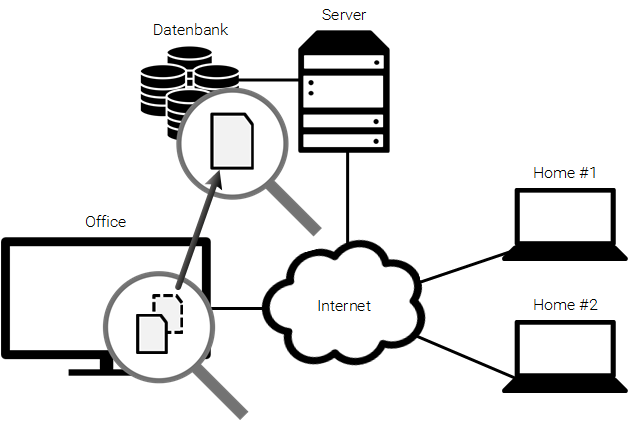
\includegraphics[]{images/Dropbox_1}
%\caption{Üblich gehandhabtes Uploaden einer Datei (wird noch geändert)}.
% TODO Grafik ändern (+ Vektor)
Bei dem Erstellen und Bearbeiten des Übungsprotokolls auf dem Schulrechner in Form
einer Text-Datei wird eine Kopie Datei auf den vom Betreiber zur Verfügung gestellten
Cloudspeicher beziehungsweise dessen Server hochgeladen und dort gespeichert.
Der Sender behält dabei die Originaldatei.

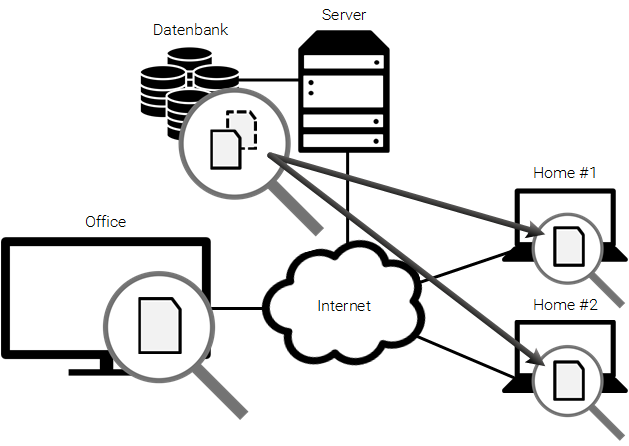
\includegraphics[]{images/Dropbox_2}
%\caption{Üblich gehandhabtes Downloaden einer Datei (wird noch geändert)}.
% TODO Grafik ändern (+ Vektor)
Wenn die Laptops Home\#1 und Home\#2 in diesem Beispiel hochgefahren sind, werden
sie über die Änderung im Cloudspeicher informiert und laden die Änderung, in
diesem Fall die neuste Version des Übungsprotokoll von dem Server herunter.
Die Text-Datei wurde somit über die zentrale Stelle, hier den Server synchronisiert.

Das Übungsprotokoll hat nach dem Synchronistationsvorgang natürlich auf den Laptops
den gleichen Inhalt wie die Datei auf dem Schulrechner, da es sich um die selbe Version
handelt. Wenn man das Übungsprotokoll nun auf einem der Laptops bearbeiten würde, würden
die neue Version genauso wie vorhin zuerst auf den Server geladen werden und vom Server
aus auf die einzelnen Clients, hier dem Schulrechner und den zweiten Laptop synchronisiert
werden und die neue Version des Übungsprotokoll überschreibt die alte.


\section{Problematik}
Einen Server als Dreh- und Angelpunkt eines Dienstes einzusetzen scheint die am
einfachsten umzusetzende und kosteneffizienteste Methode zu sein, birgt aber Sicherheitsrisiken
für den Benutzer.

In der Vergangenheit kam es schon öfters zu Hackerangriffen auf große Firmen, bei
denen große Mengen an Kundendaten gestohlen wurden. Vorfälle wie diese zeigen, wie leicht
Mengen an privaten Daten in falsche Hände fallen können, wenn diese zentral an einem Ort
gespeichert werden.

Die Speicherung privater Daten von Usern auf zentralen Servern eines Unternehmens ebnet
Geheimdiensten und staatlichen Sicherheitsbehörden außerdem den Weg, flächendeckende Überwachung
durchzuführen und damit massiv in die Privatsphäre aller User des Synchronisationsdienstes
einzugreifen, da das Unternehmen als Anbieter solcher \gls{cloudstorage} unter Umständen zur
Herausgabe der Nutzerdaten gesetzlich verpflichtet ist.

% Und selbst wenn der duchschnittliche Benutzer nichts zu verbergen hat, ist der
% dreiste Eingriff in die Privatsphäre doch als äußerst problematisch einzustufen
% und leider gestaltet sich dieser zum Bedauern der betroffenen Benutzer, für
% Fremde oft viel zu einfach.
% TODO ganz umformulieren oder weglassen
Hauptursache für diese Problematik ist die unverschlüsselte und vor allem zentrale
Speicherung der Daten.

Bei \sblit werden die angesprochenen Probleme umgangen, ohne den durch Synchronisationsdienste
gebotenen Komfort zu mindern.


\section{Lösung}
\subsection{Einleitung}
Der signifikanteste Unterschied zwischen üblichen Dateisynchronisationsdiensten
und \sblit besteht im Verzicht eines Servers. Anders als im Kapitel 1.1.2. erklärt,
findet die Kommunikation zwischen zwei Endgeräten nicht über einen Server statt,
sondern über eine direkte verschlüsselte Verbindung zwischen diesen zwei Geräten.

Durch diesen Ansatz, fällt die zentrale Sammelstelle von Nutzerdaten
weg und dem Datendiebstahl von Hackern wird ein Riegel vorgeschoben. Außerdem
wird kein betreibendes Unternehmen mehr benötigt, um Server zu warten, womit auch
die einheitliche Anlaufstelle für staatliche Sicherheitsbehörden und Geheimdienste
nicht mehr existiert.

Mit dem Weglassen eines Servers, entstehen aber auch viele ungelöste Probleme,
wenn der volle Funktionsumfang eines üblichen Dateisynchronisationsdienstes
trotzdem gewährleistet werden soll.

So fehlt der öffentliche Server als bekannter "Mittelmann" in der Kommunikation
zwischen den Clients, sodass diese sich über ein eigenes Protokoll über das
Internet hinweg finden und eine Verbindung erfolgreich aufbauen können. Mehr zu
den genauen Herausforderungen beim Verbindungsaufbau zwischen zwei Geräten und
die Bewältigung dieser gibt es im Kapitel ...
%TODO Kapitel eintragen mit verlinken.



Bei \sblit werden Dateien anstatt über einen Server, nämlich über verschlüsselte
Verbindungen zwischen zwei Endgeräten direkt übertragen.
Oft kommt es allerdings vor, dass \glspl{syncpartner} beim Verändern von
Dateien nicht erreichbar sind und keine Verbindung aufgebaut und auch
keine Datei synchronisiert werden kann.
Mit dem Senden einer neuen Version von Dateien zu warten,
bis beide Clients gleichzeitig erreichbar sind, hätte eine zu große Zeitspanne
zur Folge, in der viele Versionskonflikte auftreten könnten.
Deshalb verwendet \sblit eine Cloud, um Dateien für nicht erreichbare
Synchronisationspartner extern zwischenspeichern zu können. Die Cloud bildet
sich dabei aber nicht aus einem Server, wie üblich, sondern aus einem \gls{p2pnet}
aller Nutzer von \sblit. Diese dezentrale \gls{filecloud} wird
mit sogenannten \glspl{partnership} realisiert. Dabei geht es darum, dass sich
User, die sich gegenseitig nicht kennen müssen, einander ihre Daten direkt über
verschlüsselte Kanäle auf den Geräten des jeweiligen anderen speichern.
Um die Dateien nicht nur sicher zu übertragen, sondern auch zwischenzuspeichern,
ohne, dass Dritte Zugriff haben, werden die zu
synchronisierenden Dateien in Blöcke aufgeteilt und verschlüsselt. Diese
verschlüsselten Blöcke werden dann verteilt auf die \glspl{partnerdevice} gespeichert,
sodass diese fremden User nichts damit anfangen können, da sie weder den
Schlüssel zum Entschlüsseln, noch die Informationen über den Ort der restlichen
Blöcke besitzen. Diese befindet sich ausnahmslos nur bei dem User, zu dem die
Blöcke gehören.

\subsection{Szenario}
Bei \sblit wird der Inhalt eines Ordners synchronisert, der bei der
Konfiguration angegebenen wurde. Sobald sich Dateien innerhalb des Ordners
ändern, wird die neue Version der Datei kopiert und die Kopie wird den
erreichbaren Synchronisationspartnern über eine direkte verschlüsselte Verbindung
gesendet.

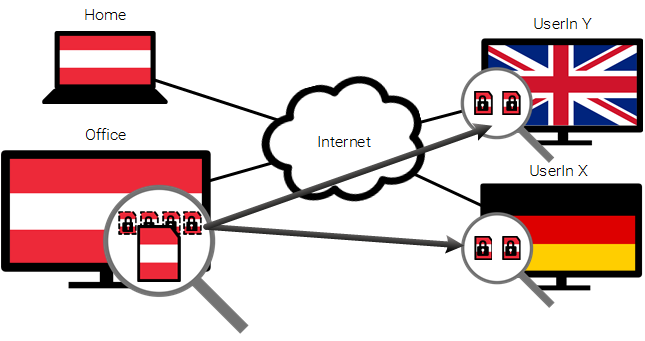
\includegraphics[]{images/sblit_1}
%\caption{Übertragung der Datei zwischen zwei erreichbaren Hosts}.

Für Synchronisationspartner, die nicht erreichbar sind, wird die Datei in der dezentralen
\gls{filecloud} zwischengespeichert. Die Datei wird kopiert und in Blöcke
aufgeteilt. Diese Blöcke werden mit dem privaten Schlüssel des Clients
verschlüsselt und verteilt auf den \glspl{partnerdevice} gespeichert.

Da die Erreichbarkeit der Partnergeräte, auf denen die veschlüsselten
Datei-Blöcke gespeichert sind, nicht gewährleistet ist, wird die Datei mehrmals
in die dezentrale \gls{filecloud} gespeichert, sodass nur ein Bruchteil der
Partnergeräte erreichbar sein muss, um auf die vollständige Datei zugreifen zu
können.

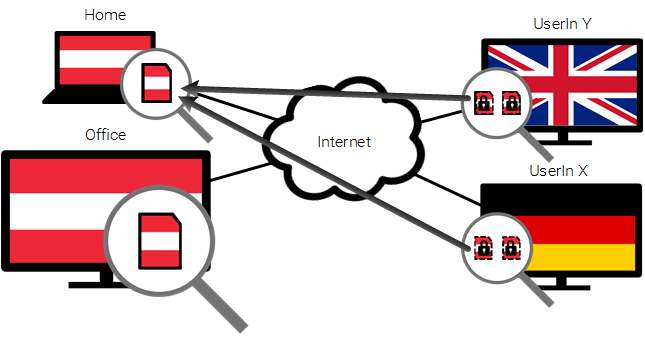
\includegraphics[]{images/sblit_2}
%\caption{Hochladen der Datei in die dezentrale \gls{filecloud}}.

Sobald der \gls{syncpartner}, hier Home wieder hochgefahren ist, fordert er die
verschlüsselten Dateiblöcke von den \glspl{partnerdevice} an. Die Blöcke werden
übertragen, entschlüsselt und zu dervollständigen Datei zusammengesetzt.

Die Datei wurde also über die Partnergeräte synchronisiert, die eine dezentrale
\gls{filecloud} darstellen.

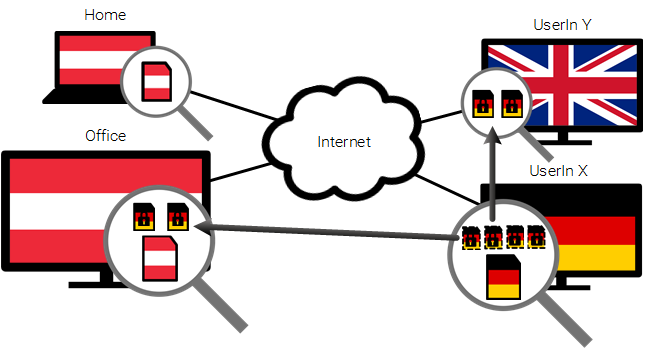
\includegraphics[]{images/sblit_3}
%\caption{Gegenseitiges Speichern von Dateiblöcken (Konzept einer \gls{partnership})}.

Im Gegenzug, dass man Daten auf Geräten anderer speichern darf, gibt man selbst
Speicherplatz für diese User frei, in dem die von ihnen verschlüsselten
Dateiblöcke zwischengespeichert werden können. Der für andere User freigegebene
Speicherplatz beträgt dabei die Speichermenge, die man selbst bei anderen Usern
beansprucht.


\chapter{Decentralized Communication Layer}\label{DCL}
\renewcommand{\kapitelautor}{Autor: Martin Exner}

\section{Einleitung}

Um die Hauptanforderung an die Umsetzung, den Verzicht auf zentrale Server im System, realisieren zu können,
wird ein \gls{p2pnet} benötigt. Über dieses läuft die Kommunikation der Synchronisationsanwendung.
Dabei muss das Netzwerk vollständig dezentral aufgebaut sein, um ohne Server funktionieren zu können.
Gleichzeitig müssen alle Teilnehmer des Netzwerks die selben Berechtigungen haben, weswegen es keinen
Teilnehmer geben kann, der besondere Befugnisse hat. Deshalb ist es notwendig, dass sich das Netzwerk
und die Teilnehmer selbst organisieren und verwalten, ohne dabei auf ein zentrales Organ angewiesen
zu sein.

Dieses \gls{p2pnet} ist in einer separaten \gls{cl}, dem \gls{dcl}, umgesetzt.
Das ermöglicht es einerseits, \gls{dcl} für Anwendungen von fremden Entwicklern zu öffnen, sodass diese auf das schon bestehende Netzwerk
zurückgreifen können und nicht erst ein eigenes umsetzen müssen, und andererseits erleichtert die klare Abgrenzung der Funktionen
zwischen \gls{cl} und eigentlicher Synchronisationsanwendung die Umsetzung beider erheblich.


\section{Anforderungen an die \gls*{cl}}

Das \gls{p2pnet} des \gls{dcl} muss eine Reihe von Eigenschaften aufweisen,
um für die Anwendung eingesetzt werden zu können. Diese Eigenschaften decken sich im wesentlichen mit
üblichen Anforderungen an herkömmliche, nicht dezentrale Netzwerke und lauten wie folgt:
\begin{description}
	\item [{Adressierung:}]
		
		Den Teilnehmern müssen eindeutige Adressen zugewiesen werden können, die auf ihre Echtheit überprüfbar sind.
	
	
	\item [{Routing:}]
		
		Zwischen Teilnehmern müssen anhand ihrer Adressen Kommunikationskanäle aufgebaut werden können.

\end{description}

Durch den dezentralen Ansatz von \gls{dcl} gestaltet sich die Realisierung dieser Eigenschaften jedoch
anders als das beispielsweise für ein übliches Computernetzwerk oder das Internet der Fall wäre.
So können Adressen nicht von zentralen, dazu bemächtigten Behörden vergeben werden und das Routing
kann nicht von speziellen Teilnehmern des Netzwerks in einer hierarchischen Organisation erfolgen.



\section{Network Types}

\subsection{Notwendigkeit}
Um \gls{dcl} für eine breite Menge an Anwendungen benutzbar zu machen, muss es möglich sein, alle
Eigenschaften, die ein \gls{p2pnet} zur Kommunikation zwischen den Instanzen dieser Anwendungen
haben muss, erfüllen zu können. Das lässt sich am besten realisieren, indem der \gls{dcl} so umgesetzt
wird, dass mehrere unterschiedliche \glspl{p2pnet} darüber aufgebaut werden können.
Das hat den Vorteil, auch mit \glslink{p2pnet}{Peer-to-Peer-Netzwerken}, die andere Anforderungen
als bisher existente \glspl{net} haben, auf die bereits bestehende Menge an Hosts aus dem \gls{dcl}
zurückgreifen zu können. So können neue \glspl{net} schnell und stabil zur Verfügung gestellt werden
und neue Teilnehmer erhöhen nicht nur die Verfügbarkeit ihres \glslink{net}{Netzwerks}, sondern auch
die aller anderer auf \gls{dcl} aufbauender \glspl{net}.

\subsection{Definition}
Ein \gls{nt} beschreibt ein \gls{net} innerhalb des \gls{dcl} durch Festlegung folgender Eigenschaften:

\begin{description}

	\descriptionitem{Adresskonzept}
		Beinhaltet die Länge von Adressen und die Verfahren zur Bildung sowie zur Überprüfung
		von Adressen.

	\descriptionitem{Routingverfahren}
		Beinhaltet den Vorgang zur Weiterleitung von Nachrichten, die an andere Teilnehmer des
		\glslink{net}{Netzwerks} adressiert sind.

\end{description}

\subsection{Notation}
Für jeden \gls{nt} gibt es einen sogenannten \gls{ntid}, mit dem er identifiziert wird.
Dieser setzt sich aus einem Typstring im Stil von Java Package Names und einem Attributstring für
Untereigenschaften zusammen.

\subsection{Circle Network}
Das im \gls{dcl} standardmäßig verwendete \gls{net} ist das \gls{cnet}. Der Typstring des \gls{nt} des
\gls{cnet} ist \code{\cnettype}.

Adressen werden im \gls{cnet} standardmäßig durch Anwendung des \gls{hash} \gls{sha1} auf öffentliche
\gls{rsa}-Schlüssel erzeugt und haben eine Länge von 20 Bytes, was der \gls{digestlength} von \gls{sha1}
entspricht.
Das Verfahren zur Bildung von Adressen im \gls{cnet} wird unter
\labellink{dcl-addr-format} auf \pagelink{dcl-addr-format} im Detail
beschrieben.

Das Format des Attributstrings des \gls{nt} des \gls{cnet} ist
\sloppy{\mbox{\code{\gls{hash}/Adresslänge}}}.
Der standardmäßige Attributstring für den \gls{nt} des \gls{cnet} ist also
\sloppy{\mbox{\code{\cnetattr}}}.

Daraus ergibt sich der standardmäßige \gls{ntid} des \gls{cnet},
\sloppy{\mbox{\code{\cnetid}}}.


\section{Adressierung}

\subsection{Notwendigkeit}
Um im \gls{dcl} Synchronisationgruppen zu bilden, ist es nötig, die Teilnehmer dieser Gruppen als solche
erkennen zu können. Das erfordert wiederum die permanente und eindeutige Adressierung dieser Teilnehmer.
Da sich die öffentlichen IP-Adressen der meisten privaten Internetanschlüsse und somit des Großteils der
Zielgruppe von \sblit periodisch ändern, eignen sich diese jedoch nicht als Adressen im \gls{dcl}. Es
wird also ein anderes Adresskonzept benötigt, mit dem ohne höhere Behörde allen Teilnehmern eindeutige
Adressen zugewiesen werden können, die auf ihre Echtheit überprüfbar sind.

Es ist nicht ausreichend, die Teilnehmer ihre Adressen willkürlich selbst bestimmen zu lassen und eine
Funktion zu implementieren, die überprüft, ob eine neu generierte Adresse im Netzwerk schon existiert,
da dieser Ansatz keinerlei Sicherheit vor einer absichtlichen Übernahme der Adresse eines anderen
Teilnehmers durch einen Angreifer bietet.

% TODO schwierigkeit: keine zentrale Stelle, Eindeutigkeit

\subsection{Adressierung mit \gls{rsa}}
\glslink{aenc}{Asymmetrische Verschlüsselungsverfahren} wie \gls{rsa} eignen sich durch ihre Eigenschaften
ausgezeichnet für die Adressierung innerhalb eines Netzwerks, in dem alle Teilnehmer die gleichen
Berechtigungen haben und in dem keine höhere Instanz existiert, die Adressen vergeben und diese
verifizieren kann.
\tags{key-info, schlüsselpaar, asymmetrisch}

Bei asymmetrischen Verschlüsselungsverfahren kommen sogenannte Schlüsselpaare, bestehend aus zwei
Schlüsseln, zum Einsatz. Die Besonderheit liegt darin, dass eine Nachricht, die mit einem Schlüssel
aus dem Schlüsselpaar verschlüsselt wurde, bei asymmetrischen Verfahren im Gegensatz zu symmetrischen
Verfahren nicht mit dem selben Schlüssel auch wieder entschlüsselt werden kann, sondern ausschließlich
mit dem anderen Schlüssel des Schlüsselpaars.
Gleichzeitig kann aus einem Schlüssel eines Schlüsselpaars der dazugehörige andere Schlüssel des
Schlüsselpaars nicht in absehbarer Zeit berechnet werden.

Dadurch wird es möglich, ein Adressierungssystem umzusetzen, das die Anforderungen im Bezug auf
Überprüfbarkeit der Adressen erfüllt. Dazu wird einer der beiden Schlüssel aus dem Schlüsselpaar
als Adresse angenommen und somit bewusst veröffentlicht, während der andere Schlüssel aus dem
Schlüsselpaar geheim gehalten wird.
Der Schlüssel aus dem Schlüsselpaar, der veröffentlicht wird, wird auch \emph{Öffentlicher Schlüssel}
oder \emph{Public Key} genannt, der weiterhin geheim gehaltene Schlüssel \emph{Privater Schlüssel} oder
\emph{Private Key}.

Öffentliche Schlüssel als Adressen haben den Vorteil, dass sie ohne höhere Behörde oder zentrale Stelle
auf ihre Echtheit überprüft werden können und somit fälschungssicher sind. Ein Mechanismus zur
Überprüfung solch einer Adresse wird im nächsten Abschnitt beschrieben.

\subsection{Überprüfung von Adressen}
Dadurch, dass eine mit einem öffentlichen Schlüssel verschlüsselte Nachricht nicht mit wieder mit dem
öffentlichen Schlüssel entschlüsselt werden kann, sondern ausschließlich mit dem dazugehörigen privaten
Schlüssel, kann der Besitz des gesamten Schlüsselpaars bewiesen werden, ohne mehr als den öffentlichen
Schlüssel preisgeben zu müssen: Eine beliebige Folge von Daten wird vom überprüfenden Teilnehmer
generiert, mit der Adresse, also dem öffentlichen Schlüssel des zu überprüfenden Teilnehmers
verschlüsselt und anschließend an diesen übermittelt. Dort wird die empfangene Nachricht vom zu
überprüfenden Teilnehmer wieder entschlüsselt und zurück an den überprüfenden Teilnehmer gesendet.
Decken sich die ursprünglich vom überprüfenden Teilnehmer generierten Daten mit denen, die vom zu
überprüfenden Teilnehmer entschlüsselt wurden, ist der Besitz des gesamten Schlüsselpaars, und nicht
lediglich des öffentlichen Schlüssels, bewiesen.

%TODO konkretes Beispiel

%TODO Erklärung der Challenge mit Nikolas mergen

\subsection{Eindeutigkeit von Adressen}
Die Eindeutigkeit der generierten \gls{rsa}-Schlüsselpaare und somit der Adressen kann zwar nicht
garantiert werden, eine Kollision ist jedoch aufgrund der Länge der verwendeten Schlüssel und der
Anzahl der dadurch möglichen Schlüsselpaare dermaßen unwahrscheinlich, dass davon ausgegangen
werden kann, dass eine Kollision praktisch nicht auftreten wird. \cite{crypto.stackexchange.com/a/2559:rsa-key-collision}



\section{Routing}

\subsection{Notwendigkeit}
Da es bereits ab einer geringen Anzahl an Teilnehmern im \gls{p2pnet} nicht mehr praktikabel ist,
ein vollständig vermaschtes Netz zu führen, weil die Anzahl an dafür notwendigen Verbindungen die
Kapazitäten der Teilnehmer überschreitet, ist es nötig, einen Routingmechanismus in das Netzwerk
zu implementieren. Damit können Nachrichten im \gls{p2pnet} von jedem Teilnehmer zu jedem beliebigen
anderen Teilnehmer gesendet werden, ohne dass die beiden kommunizierenden Teilnehmer direkt
miteinander verbunden sein müssen.

Dieses Unterkapitel beschreibt das Routing im \gls{cnet}.

\subsection{Schwierigkeit}
Im Gegensatz zu herkömmlichen Computernetzwerken sind die Verbindungen zwischen den einzelnen
Teilnehmern in einem \gls{p2pnet} variabel und ändern sich ständig. Die Wege für Pakete statisch
vorzugeben funktioniert deshalb nicht, stattdessen ist es notwendig, dynamisches Routing zu
implementieren.

Die meisten im Einsatz befindlichen Verfahren zum dynamischen Routing betrachten die gesamte
Topologie und suchen darin Wege für Pakete. Bei zu großen Topologien werden Teile des Netzwerks
zusammengefasst und die Teilnehmer innerhalb dieses Teils von Außerhalb als ein einziger Teilnehmer
betrachtet. Der Pfadfindungsprozess kann dann effizienter gestaltet werden, indem das Routing in
2 Schritten erfolgt: zuerst außerhalb bis zum zusammengefassten Teil und anschließend innerhalb
des zusammengefassten Teils des Netzwerks, wo das Routing zum endgültigen Ziel erfolgt.

Diese Technik funktioniert jedoch nur in einem hierarchisch aufgebauten Netzwerk, in dem Teilnehmer
mit ähnlichen Adressen logisch nah beieinander sind, wie das beispielsweise in einem IPv4-Subnet
der Fall ist. In einem dezentralen \gls{p2pnet}, dessen Topologie sich ständig ändert und in dem
die Adresse eines Teilnehmers nicht mit seiner Position in der Topologie zusammenhängt, können
keine Teilnehmer zusammengefasst werden.

Gleichzeitig ist die Topologie des \gls{p2pnet} so groß und ändert sich so oft, dass es praktisch 
unmöglich ist, bei jedem Teilnehmer des Netzwerks eine Kopie aller bestehenden Verbindungen zu
speichern und diese aktuell zu halten, um basierend darauf die Wege zur Weiterleitung von
Nachrichten zu finden.

\subsection{Distanzbasiertes Routing}
Im \gls{cnet} des \gls{dcl} werden nicht die Wege anhand der Topologie gesucht, sondern die
Topologie anhand der gewünschten Wege aufgebaut. Das bedeutet konkret, dass die Teilnehmer, mit
denen sich ein Teilnehmer verbindet, nicht zufällig gewählt werden, sondern ein Teilnehmer sich
tendentiell mit mehr Teilnehmern verbindet, die eine ähnliche Adresse haben, als mit solchen,
deren Adresse sich von der eigenen stark unterscheidet.

Ähnlich sind zwei Adressen dann, wenn ihre numerische Differenz gering ist. Dabei gilt es, auch
den Überlauf beim Überschreiten des mit der Adresslänge maximal darstellbaren Wertes zu beachten.
Nimmt man zur vereinfachten Darstellung eine Adresslänge von 16 Bits an, dann weisen die
hexadezimal angegebenen Adressen \code{E539} und \code{1092} eine Distanz von \code{2B59} auf,
obwohl \code{E539 - 1092 = D4A7}, weil die Distanz über den Überlauf kürzer ist:
\code{10000 - E539 + 1092 = 2B59}.

Des Weiteren werden Teilnehmer, die exakt die selbe Adresse aufweisen, stets direkt miteinander
verbunden, um sicherzustellen, dass Nachrichten deren Zieladresse auf mehrere Teilnehmer verweist,
an alle zugestellt werden. Dass zwei Teilnehmer die selbe Adresse bekommen ist jedoch erstens
extrem unwahrscheinlich und bedeutet zweitens nicht unbedingt, dass ihre Adressen auf den selben
öffentlichen Schlüsseln basieren. Siehe dazu \link{dcl-addr-uniqueness}.

Dadurch, dass die Teilnehmer des Netzwerks jeweils mehr Verbindungen zu Teilnehmern mit Adressen
ähnlich zur eigenen haben, als Verbindungen zu Teilnehmern mit Adressen, die eine hohe Differenz
zur eigenen aufweisen, können Nachrichten einfach an den Teilnehmer weitergeleitet werden, dessen
Adresse die niedrigste Differenz zur Zieladresse der Nachricht aufweist. Auf diese weise gelangt
die Nachricht, logisch betrachtet, immer näher an ihr Ziel und wird schlussendlich an den Adressat
zugestellt.

\subsection{Umsetzung im Quellcode von DCL}
Nachfolgend ist jener Teil des Quellcodes von \gls{dcl} angeführt, welcher im \code{\gls{cnt}}
zum Routinglookup angewandt wird.

\javalisting
\begin{minipage}{\linewidth}
\begin{lstlisting}[caption={Routing im \gls*{cnt} (Java)},captionpos=b]
Nexthops lookup( Data scaledDestinationAddress,
				 Address originAddress,
				 Object originIdentifierObject ) {
	Nexthops nexthops
	 = localEndpointRoutes.get(scaledDestinationAddress);
	if(nexthops != null) {
		Nexthops twinNeighbors
		 = remoteServiceRoutes.get(scaledDestinationAddress);
		if(twinNeighbors != null) {
			boolean append = true;
			for(ForwardDestination forwardDestination
				 : twinNeighbors) {
				if( forwardDestination.getIdentifierObject()
					 == originIdentifierObject ) {
					append = false;
					break;
				}
			}
			if(append) {
				nexthops.append(twinNeighbors);
			}
		}
		return nexthops;
	}
	nexthops = remoteServiceRoutes
			   .getClosest(scaledDestinationAddress);
	if(nexthops == null) {
		return null;
	}
	for(ForwardDestination forwardDestination : nexthops) {
		if(forwardDestination.getIdentifierObject()
			 == originIdentifierObject) {
			return null;
		}
	}
	return nexthops.getLast();
}
\end{lstlisting}
\end{minipage}

\begin{description}
	
	\descriptionitem{\code{scaledDestinationAddress}}
		Das \javaarg \code{scaledDestinationAddress} referenziert ein \code{\gls{Data}}-Objekt,
		welches die Zieladresse enthält, für die ein Routinglookup durchgeführt werden soll.
	
	\descriptionitem{\code{originAddress}}
		Das \javaarg \code{originAddress} referenziert ein \code{\gls{Address}}-Objekt, welches
		den öffentlichen Schlüssel des Teilnehmers enthält, von welchem die zu weiterleitende
		Nachricht empfangen wurde.
	
	\descriptionitem{\code{originIdentifierObject}}
		Das \javaarg \code{originIdentifierObject} referenziert ein Objekt, das den Teilnehmer
		identifiziert, von welchem die zu weiterleitende Nachricht empfangen wurde. Dieses wird
		benötigt, um später sicherzustellen, dass die Nachricht nicht zum selben Teilnehmer
		weitergeleitet wird, von welchem sie schon empfangen wurde.
	
	\descriptionitem{\code{\gls{Nexthops}}}
		\glsdesc{Nexthops}.
	
	\descriptionitem{\code{\gls{ForwardDestination}}}
		\glsdesc{ForwardDestination}.
	
	\descriptionitem{\code{localEndpointRoutes}}
		Die \javainstvar \code{localEndpointRoutes} referenziert ein Objekt, das zu Schlüsseln
		in Form von \code{\gls{Data}}-Objekten Werte in Form von \code{\gls{Nexthops}}-Objekten
		speichert. Dieses wird benutzt, um zu Adressen die entsprechenden
		\code{\gls{Nexthops}}-Objekte finden zu können, an die Nachrichten weitergeleitet werden
		können. In diesem Fall handelt es sich dabei ausschließlich um Adressen, deren Endpunkte
		sich am lokalen \gls{service} befinden.
	
	\descriptionitem{\code{remoteServiceRoutes}}
		Die \javainstvar \code{localEndpointRoutes} referenziert ein Objekt, das zu Schlüsseln
		in Form von \code{\gls{Data}}-Objekten Werte in Form von \code{\gls{Nexthops}}-Objekten
		speichert. Dieses wird benutzt, um zu Adressen die entsprechenden
		\code{\gls{Nexthops}}-Objekte finden zu können, an die Nachrichten weitergeleitet werden
		können. In diesem Fall handelt es sich dabei ausschließlich um Adressen, deren Endpunkte
		sich auf direkt verbundenen, aber nicht am lokalen \gls{service} befinden.
	
\end{description}

Mit \code{localEndpointRoutes.get(scaledDestinationAddress)} wird zu Beginn des Routinglookups
nach lokalen \glslink{endp}{Endpunkten} mit der genauen Zieladresse dieser Nachricht gesucht.
Werden ein oder mehrere \glspl{endp} gefunden, so wird weiters geprüft, ob es entfernte Endpunkte
gibt, die die selbe Adresse haben. Gibt es solche \glspl{endp}, dann wird sichergestellt, dass
keiner dieser \glspl{endp} derjenige \gls{endp} ist, von dem die Nachricht empfangen wurde und
dass die Nachricht somit nicht wieder zu diesem \gls{endp} weitergeleitet wird.
Anschließend werden die \glspl{endp} mit der gleichen Adresse wie der lokale \gls{endp} zur Liste
der \glspl{endp}, an die die Nachricht weitergeleitet werden soll, hinzugefügt.
Das geschieht, indem das von \code{twinNexthops} referenzierte \code{\gls{Nexthops}}-Objekt
mit \code{nexthops.append(twinNexthops)} an das von \code{nexthops} referenzierte
\code{\gls{Nexthops}}-Objekt angehängt wird.

Wurden keine lokalen \glspl{endp} mit der Zieladresse der Nachricht gefunden, dann wird mit
\code{remoteServiceRoutes.getClosest(scaledDestinationAddress)} nach direkt verbundenen
\glslink{endp}{Endpunkten} gesucht, deren Adresse der Zieladresse am ähnlichsten ist.
Anschließend wird, wie schon bei den lokalen \glslink{endp}{Endpunkten}, sichergestellt,
dass die Liste von \glspl{endp} nicht den \gls{endp} enthält, von dem die Nachricht empfangen
wurde.
Falls das der Fall ist, wird \code{null} zurückgegeben und die Nachricht in Folge verworfen.

Anderenfalls wird nur der letzte \gls{endp} in der von \code{nexthops} referenzierten
Liste der \glspl{endp} zurückgegeben: Enthält die Liste mehrere Einträge, so haben die darin
enthaltenen \glspl{endp} die selbe Adresse. Die Nachricht soll in diesem Fall abernur an einen
dieser \glspl{endp} weitergeleitet werden, da sie von dort an die restlichen \glspl{endp} mit der
gleichen Adresse weitergeleitet wird.






\section{NAT-Traversal}

\label{dcl-natt}

\subsection{Einleitung}
Unter \gls{nat} versteht man das Übersetzen von Netzwerkadressen.
\Gls{nat} kommt bei praktisch allen Routern privater Internetanschlüsse zum
Einsatz und ermöglicht es dort, mehrere Hosts über eine einzige öffentliche
IP-Adresse an das Internet anzubinden.

Realisiert wird das durch Übersetzen der privaten Quell-IP-Adressen zur
öffentlichen IP-Adresse bei Paketen die das lokale Netzwerk verlassen und
Rückübersetzen der öffentlichen Ziel-IP-Adresse zu den privaten IP-Adressen
bei Paketen die aus dem Internet in das lokale Netzwerk eintreten.

Bei ankommenden Paketen wird dabei anhand des Ziel-Ports entschieden, an welche
lokale IP-Adresse das Paket weitergeleitet wird.
Um es mehreren lokalen Hosts zu ermöglichen, vom gleichen Port aus Pakete zu
senden, werden die Quell-Ports von Paketen die das lokale Netzwerk verlassen
gegebenenfalls, zusätzlich zur Quell-IP-Adresse, ebenfalls übersetzt.
Beim Eintritt von Antwortpaketen in das lokale Netzwerk werden die Ziel-Ports
entsprechend Rückübersetzt. Man spricht dann von der sogenannten Port Address
Translation, die eine Unterkategorie der \acrlong{nat} bildet.

Im \gls{natdev} werden die aktuellen Übersetzungen in einer Datenstruktur
gespeichert, die lokale IP-Adressen und Ports auf globale IP-Adressen und Ports
abbildet.
Dabei werden Datenreihen im folgenden Format gespeichert:

\begin{equation*}
    (\text{ lokale IP-Adresse}, \text{ lokaler Port}, \text{ globale IP-Adresse}, \text{ globaler Port })
\end{equation*}

Verlässt beispielsweise ein Paket das lokale Netzwerk, das von der lokalen
IP-Adresse \code{10.0.0.1} und vom Port \code{28785} aus gesendet wurde,
könnte die dafür von einem \gls{natdev} mit der öffentlichen IP-Adresse
\code{93.184.216.34} angelegte Datenreihe wie folgt aussehen:

\begin{equation*}
    (\texttt{ 10.0.0.1}, \texttt{ 28785}, \texttt{ 93.184.216.34}, \texttt{ 28785 })
\end{equation*}

An dieser Stelle sei angemerkt, dass der Quellport des Pakets in diesem Beispiel
nicht übersetzt wird.
Ist der Host mit der IP-Adresse \code{10.0.0.1} der einzige im lokalen Netzwerk,
der von Port \code{28785} aus sendet, muss eine Übersetzung des Ports auch nicht
zwingend stattfinden.
Nimmt man jedoch an, dass sich ein zweiter Host im lokalen Netzwerk befindet,
der beispielsweise die IP-Adresse \code{10.0.0.2} besitzt und ebenfalls von Port
\code{28785} aus sendet, so würde eine weitere Datenreihe angelegt, die wie
folgt aussieht:

\begin{equation*}
    (\texttt{ 10.0.0.2}, \texttt{ 28785}, \texttt{ 93.184.216.34}, \texttt{ 28786 })
\end{equation*}

Für Pakete des Hosts mit der IP-Adresse \code{10.0.0.2}, die das lokale Netzwerk
verlassen, wird also nicht nur die Quell-IP-Adresse übersetzt, sondern auch der
Quellport von \code{28785} auf \code{28786}. Dieser Schritt ist notwendig, da
sonst bei Paketen, die aus dem Internet in das lokale Netzwerk eintreten, nicht
unterschieden werden kann, ob diese an den Host mit der IP-Adresse
\code{10.0.0.1} oder an den Host mit der IP-Adresse \code{10.0.0.2}
weitergeleitet werden sollen. Die Übersetzung des Quellports ermöglicht es,
das lokale Ziel von Antwortpaketen anhand deren Zielport zu bestimmen.

%TODO erwähnen, dass öffentliche IP+Port bei unterschiedlichen Zielen gleich
%bleibt?

\subsection{Probleme für Peer-to-Peer-Verbindungen}
Verbindungen zwischen zwei über \glspl{natdev} angebundenen Hosts werden durch
\acrlong{nat} erschwert, da die Pakete zur Initialisierung der Verbindung
aufgrund fehlender Übersetzungsinformationen in den
\glslink{natdev}{NAT-Geräten} nicht an den Zielhost weitergeleitet werden
können.

Um trotzdem Peer-to-Peer-Verbindungen zwischen solchen Hosts aufbauen zu können,
müssen Verfahren zum \gls{natt} angewandt werden.
Hierfür existieren unterschiedliche Protokolle zur Einrichtung einer
Portweiterleitung auf dem lokalen \gls{natdev}, welche eine Verbindung von Außen
ermöglicht.

Die derzeitige Implementierung des \gls{service} wendet das sogenannte
\gls{nathp} an, für das kein spezielles Netzwerkprotokoll notwendig ist.

\subsection{NAT Hole Punching}
Für \gls{nathp} wird für eine neue Verbindung ein Kommunikationskanal zwischen
den Verbindungspartnern benötigt, der schon vor Aufbau der Verbindung existieren
muss.
Diesen Kommunikationskanal kann ein dritter Host bereitstellen, zu dem beide
Verbindungspartner bereits verbunden sind, oder, wie im Fall von \gls{dcl},
ein \glslink{net}{DCL-Netzwerk}, über das beide Kommunikationspartner bereits
kommunizieren können.
In beiden Fällen muss bereits eine Verbindung zu einem Host außerhalb des
lokalen Netzwerks bestehen.

Einer der beiden Hosts, die direkt miteinander verbunden werden sollen,
ermittelt seine öffentliche IP-Adresse und seinen öffentlichen Port mithilfe
eines Hosts, zu dem bereits eine Verbindung besteht.
Diese Information wird über den bestehenden Kommunikationskanal an den Host
übermittelt, zu dem eine Verbindung aufgebaut werden soll.
Dieser sendet an die eben erhaltene Adresse ein Paket, das das lokale Netzwerk
zwar verlässt, am \gls{natdev} des Ziels jedoch verworfen wird.
Der Grund dafür liegt darin, dass das Ziel, an das es im lokalen Netzwerk der
Empfängerseite weitergeleitet werden soll, vom dortigen \gls{natdev} nicht
bestimmt werden kann, da kein passender Eintrag in der Datenstruktur der
Übersetzungen existiert.
Das \gls{natdev} auf der Senderseite dieses Pakets erstellt jedoch trotzdem
einen Übersetzungseintrag in seiner Datenstruktur, um Antwortpakete weiterleiten
zu können.

Gleichzeitig ermittelt dieser Host über einen anderen Host, zu dem bereits eine
Verbindung besteht, ebenfalls seine öffentlichen Adresse.
Diese sendet er zusätzlich zu dem soeben in der Übertragung gescheiterten Paket
über den bestehenden Kommunikationskanal an den ersten Verbindungspartner.

Dieser sendet, sobald er die öffentliche Adresse des Gegenübers empfangen hat,
ein normales Paket zur Verbindungsinitialisierung an dieses Gegenüber.
Dieses Paket verlässt das lokale Netzwerk, das lokale \gls{natdev} speichert
einen Übersetzungseintrag in seiner Datenstruktur und das Paket erreicht das
entfernte \gls{natdev}.
Dort wird jener Übersetzungseintrag gefunden, der durch das in der Übertragung
bewusst gescheiterte Paket angelegt wurde.
Das Paket wird anhand dieses Eintrags an den richtigen Host weitergeleitet und
die Hosts können ab diesem Zeitpunkt normal miteinander kommunizieren.

\subsection{Einschränkungen}
Um \gls{nathp} durchführen zu können, muss jedenfalls bereits mindestens eine
Verbindung zu einem Host außerhalb des lokalen Netzwerks existieren.
Die erste Verbindung, die ein über ein \gls{natdev} angebundenes Gerät aufbaut,
muss deshalb jedenfalls zu einem Host erfolgen, der selbst nicht über ein
\gls{natdev} angebunden ist und somit Verbindungen problemlos annehmen kann.
Im Fall von \gls{dcl} sind das \glspl{service}, die auf Hosts laufen, die dieses
Kriterium erfüllen und zusätzlich über eine statische IP-Adresse verfügen.
In der Praxis handelt es sich bei diesen Hosts um Server.
Um einen möglichst problemlosen Einstieg in den \gls{dcl} gewährleisten zu
können, ist es nötig, auf eine der Anzahl an Teilnehmern im \gls{dcl}
entsprechend große Menge an \glspl{service} zurückgreifen zu können, die auf
solchen Hosts laufen.


\section{Links}

\label{dcl-link}

\subsection{Einleitung}
Um \gls{natt} möglichst problemlos durchführen zu können, erfolgt die
Kommunikation zwischen \glspl{service} über das \gls{udp}.
Da \gls{udp} selbst jedoch keine verlässliche Übertragung und keine
Verschlüsselung bietet, werden die Datenströme zwischen \glspl{service} über
\glspl{link} übertragen.
Diese gewährleisten die verlässliche und geordnete Übertragung der Daten,
außerdem wird der Übertragungskanal verschlüsselt.

\subsection{Sicherheit}
\Glspl{link} werden mit dem \gls{aes} im \gls{gcm} verschlüsselt.
Das garantiert sowohl Vertraulichkeit, Authentizität als auch Integrität der
verschlüsselten Daten.

\subsection{Channels}
\label{dcl-link-channels}
Über einen \gls{link} können mehrere getrennte Datenströme gleichzeitig
übertragen werden. Um diese voneinander abzugrenzen, werden sie in
unterschiedlichen \glspl{channel} übertragen.

Auch die zur Verwaltung des \glslink{link}{Links} notwendigen Nachrichten
werden in einem \gls{channel}, dem \gls{mgmtch}, übertragen.

Der Link selbst definiert deshalb nur eine einzige Message, die Daten, einen
\gls{channelid} für die Zuweisung dieser Daten zu einem \gls{channel} und einen
\gls{dataid} für die Angabe der Reihenfolge dieser Daten innerhalb des
\glslink{channel}{Channels} überträgt.
Siehe dazu \figurelink{dcl-link-bytefield}.
Für \gls{fnumc}, siehe \link{dcl-packetcomponents-flexnum}.

\linkbytefield

Die Messages zur Verwaltung des \glslink{link}{Links} definiert das verwendete
\gls{mcp}.
Für die Initialisierung des \glslink{link}{Links} werden die Messages des
\gls{bmcp} verwendet.
\gls{bmcp} definiert aber auch Messages für den späteren Wechsel des verwendeten
\gls{mcp}.

\subsection{Basic Management Channel Protocol}
\label{dcl-link-bmcp}

\subsubsection{Einleitung}
Das \acrfull{bmcp} ist das standardmäßig verwendete \gls{mcp} für
\glslink{link}{Links}.
Es definiert Messages und Abläufe zum Aufbau der Verbindung, zum Öffnen von
\glspl{channel}, zur erneuten Übertragung von verlorenen Nachrichten und zur
\gls{fcnt}.

\subsubsection{Initialisierung}
Während der Initialisierung eines \glslink{link}{Links} wird entschieden, wie
dieser \gls{link} verschlüsselt wird und wie diese Verschlüsselung initialisiert
wird.
Der Initiator des \glslink{link}{Links} sendet dazu in der \msg{\bmcpconnectreq}
eine Liste an möglichen \glspl{cinitmethod}, aus der der Empfänger eine wählt
und diese in der \msg{\bmcpconnectrep} bestätigt.
Danach werden, je nach \gls{cinitmethod} unterschiedlich, eine Reihe an
\msgpl{\bmcpcryptoinit} gesendet, bis die Verschlüsselung initialisiert ist.
Zur Zeit existiert nur eine \gls{cinitmethod}: \gls{aes}/\gls{gcm} via
\gls{rsa}.
Bei dieser \gls{cinitmethod} werden, nach Austausch der öffentlichen
\gls{rsa}-Schlüssel, zufällig generierte \gls{aes}-Schlüssel mit den
öffentlichen \gls{rsa}-Schlüsseln verschlüsselt, übertragen und angewandt.

Für eine spätere Implementierung ist eine zusätzliche \gls{cinitmethod} geplant,
die die \gls{aes}-Schlüssel über das Diffie-Hellman-Merkle
Schlüsselaustauschverfahren generiert.

\subsubsection{Messageaufbau}
Die Messages des \acrlong{bmcp} sind generell so aufgebaut, dass ein einzelnes
Byte am Beginn der Message deren Typ angibt, anhand dessen die restliche
Nachricht interpretiert wird.

\bmcpbytefield

\subsubsection{Messages}

\subsubsection*{Connect Request}
\label{dcl-bmcp-connectreq}
Die \msg{\bmcpconnectreq} ist die Message zur Verbindungsanfrage und folglich
die erste Message eines \glslink{link}{Links}, die übertragen wird.
Die Message enthält eine Liste an \glspl{cimid} jener \glspl{cinitmethod}, die
der Sender akzeptiert.
Der Empfänger antwortet bei Annahme der Verbindung mit einer
\msg{\bmcpconnectrep}, die einen der angeführten \glspl{cimid} enthält.

\bmcpconnectreqbytefield


\subsubsection*{Connect Reply}
\label{dcl-bmcp-connectrep}
Die \msg{\bmcpconnectrep} wird als Antwort auf eine vorhergehende
\msg{\bmcpconnectreq} gesendet und enthält einen der darin angeführten
\glspl{cimid}.
Dieser bestimmt, wie der \gls{link} verschlüsselt wird und wie diese
Verschlüsselung initialisiert wird.
Zum weiteren Verbindungsaufbau folgt, je nach verwendeter \gls{cinitmethod},
eine Reihe an \msgpl{\bmcpcryptoinit}.

\bmcpconnectrepbytefield


\subsubsection*{Disconnect}
\label{dcl-bmcp-disconnect}
Die \msg{\bmcpdisconnect} dient zur Beendigung des \glslink{link}{Links}.
Der Empfänger bestätigt die Auflösung der Verbindung durch Senden einer
\msg{\bmcpkill}.

\bmcpdisconnectbytefield


\subsubsection*{Kill}
\label{dcl-bmcp-kill}
Die \msg{\bmcpkill} ist die letzte Nachricht eines \glslink{link}{Links}, die
übertragen wird, und markiert das Ende der Verbindung.
Die Message wird als Antwort auf eine \msg{\bmcpdisconnect} gesendet, kann aber
bei unerwartetem Beenden des \glslink{link}{Links} durch einen
Verbindungspartner auch alleinstehend gesendet werden.

\bmcpkillbytefield


\subsubsection*{Crypto Init}
\label{dcl-bmcp-cryptoinit}
Die \msg{\bmcpcryptoinit} überträgt Daten zur Initialisierung der verwendeten
Verschlüsselung des \glslink{link}{Links} und wird zu Beginn der Verbindung, je
nach verwendeter \gls{cinitmethod}, unterschiedlich oft übertragen.

\bmcpcryptoinitbytefield


\subsubsection*{Ack}
\label{dcl-bmcp-ack}
Die \msg{\bmcpack} dient zur Bestätigung empfangener Anfragen, wie
beispielsweise einer \msg{\bmcpopenchreq}.
Die Message enthält den \gls{dataid} der bestätigten Anfrage.

\bmcpackbytefield


\subsubsection*{Change Protocol Request}
\label{dcl-bmcp-chprotoreq}
Die \msg{\bmcpchprotoreq} dient zum Wechsel des verwendeten \gls{mcp}.
Die Message enthält einen \gls{protoid} in Form eines Strings, der das neue
\gls{mcp} angibt.
Der Empfänger bestätigt den Wechsel des Protokolls mit einer \msg{\bmcpack},
die den \gls{dataid} dieser \msg{\bmcpchprotoreq} enthält.

\bmcpchprotoreqbytefield


\subsubsection*{Channel Block Status Request}
\label{dcl-bmcp-chblockstatreq}
Die \msg{\bmcpchblockstatreq} dient zur Abfrage der empfangenen \glspl{dataid}
eines oder mehrerer \glslink{channel}{Channels}.
Die Message enthält eine Liste der \glspl{channelid} der \glspl{channel}, die
abgefragt werden sollen.

Der Empfänger antwortet mit einer \msg{\bmcpchblockstatrep}, anhand der der
Sender dieser \msg{\bmcpchblockstatreq} feststellen kann, welche Pakete nicht
am Ziel angekommen sind und erneut übertragen werden müssen.

\bmcpchblockstatreqbytefieldattr{htb}


\subsubsection*{Channel Block Status Report}
\label{dcl-bmcp-chblockstatrep}
Die \msg{\bmcpchblockstatrep} wird als Antwort auf eine
\msg{\bmcpchblockstatreq} gesendet und enthält eine Liste an
\glspl{chblockstatrep} für jeden der in der Anfrage angeführten \glspl{channel}.
Der Empfänger kann anhand dieser \glspl{chblockstatrep} erkennen, welche Pakete
nicht übertragen wurden und deshalb erneut gesendet werden müssen.

Ein \gls{chblockstatrep} enthält den \gls{channelid} des
\glslink{channel}{Channels}, auf den er sich bezieht,
den niedrigsten und den höchsten \gls{dataid}, die auf diesem \gls{channel}
empfangen wurden, % TODO die empfangen wurden oder der empfangen wurde?
die Anzahl an unterschiedlichen \glspl{dataid}, die insgesamt auf diesem
\gls{channel} empfangen wurden
und je eine Liste an nicht empfangenen, einzelnen \glspl{dataid} sowie an
zusammenhängenden Blöcken aus nicht empfangenen \glspl{dataid} innerhalb des
niedrigsten und höchsten \glslink{dataid}{Data Identifiers} des
\glslink{channel}{Channels}.

\bmcpchblockstatrepbytefield


\subsubsection*{Open Channel Request}
\label{dcl-bmcp-openchreq}
Die \msg{\bmcpopenchreq} dient zur Anfrage über das Öffnen eines neuen
\glslink{channel}{Channels}.
Die Message enthält den \gls{channelid} des neuen \glslink{channel}{Channels}
sowie den \gls{protoid} des Protokolls, über das auf dem neuen \gls{channel}
kommuniziert werden soll.

Nimmt der Empfänger die Anfrage an, wird eine \msg{\bmcpack} gesendet, die den
\gls{dataid} dieser \msg{\bmcpopenchreq} enthält.

\bmcpopenchreqbytefieldattr{htb}


\subsubsection*{Throttle}
\label{dcl-bmcp-throttle}
Die \msg{\bmcpthrottle} dient zur Limitierung der Sendeübertragungsrate des
Empfängers und wird für die \gls{fcnt} des \glslink{link}{Links} genutzt.
Die Message enthält die maximal zulässige Senderate in Bytes pro Sekunde.

\bmcpthrottlebytefieldattr{htb}


\section{Interservice-Protokoll}

\subsection{Einleitung}
Das \gls{isproto} wird zur Kommunikation zwischen zwei direkt miteinander verbundenen \glspl{service}
verwendet.
Es dient zur Übertragung von zwischen Anwendungen gesendeten Nachrichten, zur
Bekanntgabe von \glslink{endp}{Endpunkten} samt Adressen und beigetretenen
\glslink{net}{Netzwerken}, sowie zum Einstieg in \glspl{net} des \gls{dcl}.

Die Messages des \glslink{isproto}{Interservice-Protokolls} werden über den
\gls{isch}, einen \gls{channel} des \glslink{link}{Links} zwischen zwei
\glspl{service}, übertragen. Der \gls{protoid} des
\glslink{isproto}{Interservice-Protokolls} ist \code{org.dclayer.interservice}.

Dieses Unterkapitel beschreibt das \gls{isproto} in Version 0.

\subsection{Address Slots}
Da \glspl{service} jeweils mehrere Adressen hosten können, ist es notwendig, diese mit dem
\gls{isproto} unterscheiden zu können. Jede Adresse wird hierbei einem eigenen \gls{addrslot}
zugeordnet, um sich in den Messages des Protokolls einfach auf einzelne Adressen beziehen zu können,
ohne jedes mal die ganze Adresse senden zu müssen.
%TODO Übergang zu connection base; Verbindung Addr Slots <-> Net Slots

\subsection{Network Slots}
Eine Adresse kann gleichzeitig in mehreren verschiedenen \glslink{net}{Netzwerken} vertreten sein. Um diese
\glspl{net} in den Messages des \gls{isproto} einfach referenzieren zu können, ohne jedes mal den
ganzen \gls{ntid} übertragen und parsen zu müssen, wird jedes \gls{net}, dem ein \gls{service} mit einer
oder mehreren Adressen beitritt einem \gls{netslot} zugeordnet.

Werden Nachrichten zur Kommunikation zwischen Anwendungen, sogenannte
\glspl{netpkt}, über den \gls{isch} übertragen, so wird auch das \gls{net}, in
dem diese geroutet werden, in Form des entsprechenden \gls{netslot} angeführt,
um beim Empfänger die Zuordnung zu ermöglichen.

\subsection{Connection Base}
Die \gls{connbase} gibt an, welche Messages von einem \gls{service} auf einem \gls{addrslot} eines
\gls{isch} akzeptiert werden. Derzeit sind zwei Werte für die \gls{connbase} implementiert:
\const{stranger} (\code{0}) und \const{trusted} (\code{1}).
Ein neuer \gls{addrslot} wird immer mit der \gls{connbase} \const{stranger} initialisiert, unter
welcher keine mit dem Routing in Verbindung stehenden Messages akzeptiert werden.
Erst ab der \gls{connbase} \const{trusted} werden Messages akzeptiert, die auf
das Routing Einfluss nehmen.
Konkret handelt es sich dabei um die \msg{\isprotonjn}, die \msg{\isprotonln},
die \msg{\isprotonp}, die \msg{\isprotoireq}, die \msg{\isprotoacsa} und die
\msg{\isprotoacd}.

Als Voraussetzung für die \gls{connbase} \const{trusted} gilt der Beweis der Adresse dieses
\glslink{addrslot}{Address Slots}. Ein \gls{service} kann den Wechsel auf die \gls{connbase}
\const{trusted} für einen existenten \gls{addrslot} anfordern, indem er eine \msg{\isprotots}
an sein Gegenüber sendet.
Der entfernte \gls{service} fordert den lokalen \gls{service} danach durch Senden einer
\msg{\isprotoccreq} auf, mit seiner Adresse eine \gls{cchlg} zu lösen, um ihre Echtheit zu
beweisen. Siehe dazu \link{dcl-addr-proving}.
Der lokale \gls{service} antwortet mit einer \msg{\isprotoccrep} und übermittelt die Daten der
gelösten \gls{cchlg} an den entfernten \gls{service}.
Ist die Lösung der \gls{cchlg} korrekt, so wird die \gls{connbase} des
\glslink{addrslot}{Address Slots} auf \const{trusted} gesetzt und der lokale \gls{service} mit
einer \msg{\isprotocbn} über die geänderte \gls{connbase} benachrichtigt.

Erst jetzt akzeptiert der entfernte \gls{service} vom lokalen \gls{service} gesendete
\msgpl{\isprotonjn} und \msgpl{\isprotonln}.

Die Aufforderung zum Weiterleiten von \glspl{netpkt} durch die \msg{\isprotonp} wird nur
akzeptiert, wenn der sendende \gls{service} dem \gls{net}, das vom \gls{netslot} in der
\msg{\isprotonp} referenziert wird, zuvor mit mindestens einer Adresse beigetreten ist.
Das erfordert wiederum die Übertragung einer \msg{\isprotonjn}, für welche die \gls{connbase}
\const{trusted} notwendig ist.

Die Anforderung von \glspl{lla} geeigneter Nachbarn kann vom Gegenüber ebenfalls erst dann
bearbeitet werden, wenn der sendende \gls{service} zuvor zumindest einem \gls{net} mit zumindest
einer Adresse beigetreten ist.
Das erfordert ebenfalls wiederum die Übertragung einer \msg{\isprotonjn}, für welche die
\gls{connbase} \const{trusted} notwendig ist.

Damit die Aufforderung zum Weiterleiten von in einem \gls{appch} übertragenen Daten akzeptiert
werden kann, muss der in der \msg{\isprotoacd} angeführte \gls{appchslot} existieren. Dafür
muss dieser zuvor mit einer \msg{\isprotoacsa} angelegt worden sein, wofür
ebenfalls die \gls{connbase} \const{trusted} notwendig ist.

\subsection{Initialisierung}
Die Kommunikation über das \gls{isproto} wird mit der Aushandlung einer Protokollversion begonnen.
Dazu werden, beginnend mit dem Initiator, also dem \gls{service}, der die Verbindung angefordert hat,
so lange \msgpl{\isprotoversion} abwechselnd zwischen den \glspl{service} gesendet, bis die letzten
zwei übertragenen \msgpl{\isprotoversion} die selben Versionsnummern enthalten.

\subsection{Messageaufbau}
Eine Message im \gls{isproto} ist generell so aufgebaut, dass ein \gls{fnumc} am Anfang der
Message den Typ angibt, anhand dessen die restliche Nachricht interpretiert wird.

\Glspl{fnumc} werden unter \labellink{dcl-packetcomponents-flexnum} auf
\pagelink{dcl-packetcomponents-flexnum} beschrieben.

\isprotobytefield

\subsection{Messages}

\subsubsection{Version}
\label{dcl-isproto-version}
Die \msg{\isprotoversion} enthält eine Versionsnummer in Form eines FlexNum-Components und wird
benutzt, um am Beginn der Verbindung die verwendete Version des \gls{isproto} auszuhandeln.

\isprotoversionbytefield

\subsubsection{LLA Request}
\label{dcl-isproto-llareq}
Die \msg{\isprotollareq} wird benutzt, um vom Gegenüber eine Liste an \glspl{lla} von anderen
\glspl{service} anzufordern.
Die Message enthält ein Feld für die Maximalanzahl an \glspl{lla}, die in der
\msg{\isprotollarep} zurückgesendet werden sollen.

Diese Message stellt keine Anforderungen an die aktuelle \gls{connbase}.

\isprotollareqbytefield


\subsubsection{LLA Reply}
\label{dcl-isproto-llarep}
Die \msg{\isprotollarep} wird als Antwort auf eine zuvor empfangene \msg{\isprotollareq} gesendet
und enthält \glspl{lla} von anderen \glspl{service}.

\isprotollarepbytefield


\subsubsection{Trusted Switch}
\label{dcl-isproto-ts}
Die \msg{\isprotots} wird benutzt, um vom Gegenüber eine \gls{cchlg} für den als Adresse verwendeten,
angegebenen öffentlichen Schlüssel anzufordern. Dieser Schritt wird benötigt, um dem Gegenüber beweisen
zu können, dass die angegebene Adresse echt ist. Erst wenn die \gls{cchlg} erfolgreich durchgeführt
wurde, kann der Sender der \msg{\isprotots} damit am Routing jener \glspl{net} teilnehmen, denen er
mit der angegebenen Adresse beigetreten ist.
% TODO: "Erst wenn X, kann Y" oder "Erst wenn X kann Y"? (Beistrich)

Mit dieser Nachricht wird gleichzeitig die in Form eines öffentlichen Schlüssel angegebene Adresse
mit dem angegebenen \gls{addrslot} assoziiert.

Diese Message stellt keine Anforderungen an die aktuelle \gls{connbase}.

\isprototsbytefield


\subsubsection{Crypto Challenge Request}
\label{dcl-isproto-ccreq}
Die \msg{\isprotoccreq} wird als Antwort auf eine \msg{\isprotots} gesendet und fordert das Gegenüber
auf, die enthaltenen Binärdaten im Rahmen einer \gls{cchlg} mit dem zur angegebenen Adresse
zugehörigen privaten Schlüssel zu signieren.

Diese Message wird vom Empfänger nur dann akzeptiert, wenn sie zuvor durch Senden einer
\msg{\isprotots} angefordert wurde.

\isprotoccreqbytefield


\subsubsection{Crypto Challenge Reply}
\label{dcl-isproto-ccrep}
Die \msg{\isprotoccrep} wird als Antwort auf eine \msg{\isprotoccreq} gesendet und enthält die Daten
der gelösten \gls{cchlg}.

Diese Message wird vom Empfänger nur dann akzeptiert, wenn sie zuvor durch Senden einer
\msg{\isprotoccreq} angefordert wurde.

\isprotoccrepbytefield


\subsubsection{Connection Base Notice}
\label{dcl-isproto-cbn}
Die \msg{\isprotocbn} wird als Antwort auf eine \msg{\isprotoccrep} gesendet und benachrichtigt
den Empfänger über die aktuelle \gls{connbase} der vom angegebenen \gls{addrslot} referenzierten
Adresse.

Diese Message stellt keine Anforderungen an die aktuelle \gls{connbase} und kann auch gesendet
werden, ohne vorher angefordert worden zu sein.

\isprotocbnbytefield


\subsubsection{Network Join Notice}
\label{dcl-isproto-njn}
Die \msg{\isprotonjn} benachrichtigt den Empfänger darüber, dass der sendende \gls{service} mit der
vom angegebenen \gls{addrslot} referenzierten Adresse dem vom angegebenen \gls{netslot} referenzierten
\gls{net} beigetreten ist. Sollte der sendende \gls{service} diesem \gls{net} zuvor noch mit keiner
Adresse beigetreten sein, so wird dieser \gls{netslot} mit dieser Message angelegt. Das von diesem
\gls{netslot} referenzierte \gls{net} wird durch den angegebenen \gls{ntid} spezifiziert.
Der Empfänger wird in diesem Fall mit dieser Nachricht außerdem darüber in Kenntnis gesetzt, dass
ab jetzt Nachrichten zum Routing in diesem \gls{net} an den sendenden \gls{service} übermittelt
werden können.
Das Feld des \gls{ntid} bleibt in den folgenden \msgpl{\isprotonjn}, die sich auf den angegeben
\gls{netslot} beziehen, leer.

Diese Message wird vom Empfänger nur dann akzeptiert, wenn die \gls{connbase} des angegebenen
\gls{addrslot} mindestens \const{trusted} entspricht.

\isprotonjnbytefield

\subsubsection{Network Leave Notice}
\label{dcl-isproto-nln}
Die \msg{\isprotonln} benachrichtigt den Empfänger darüber, dass der sendende \gls{service} mit der
vom angegebenen \gls{addrslot} referenzierten Adresse aus dem vom angegebenen \gls{netslot}
referenzierten \gls{net} austritt. Sollte der sendende \gls{service} aktuell mit keiner anderen
Adresse diesem \gls{net} beigetreten sein, so wird der Empfänger mit dieser Nachricht außerdem
darüber in Kenntnis gesetzt, dass ab jetzt keine Nachrichten mehr zum Routing in diesem \gls{net}
an den Sender übermittelt werden können.

Diese Message wird vom Empfänger nur dann akzeptiert, wenn die \gls{connbase} des angegebenen
\gls{addrslot} mindestens \const{trusted} entspricht.

\isprotonlnbytefield


\subsubsection{Integration Request}
\label{dcl-isproto-ireq}
Die \msg{\isprotoireq} fordert den Empfänger auf, den sendenden \gls{service} in die gemeinsamen
\glspl{net} zu integrieren. Konkret bedeut das, dafür zu sorgen, dass der sendende \gls{service}
so mit anderen \glspl{service} verbunden wird, dass das Routing der Adressen des sendenden
\gls{service} möglichst effizient funktionieren kann.

Diese Message wird vom Empfänger nur dann akzeptiert, wenn der sendende \gls{service} zuvor mit
mindestens einer Adresse mindestens einem \gls{net} beigetreten ist.

\isprotoireqbytefield


\subsubsection{Integration Connect Request}
\label{dcl-isproto-icreq}
Die \msg{\isprotoicreq} fordert den Empfänger auf, eine Verbindung zur angegebenen \gls{lla}
aufzubauen und wird als Antwort auf eine frühere \msg{\isprotoireq} gesendet. Sie wird benötigt,
um neue Teilnehmer eines \glslink{net}{Netzwerks} mit ihren entsprechenden Nachbarn verbinden zu
können.

Diese Message wird vom Empfänger nur dann akzeptiert, wenn sie zuvor durch Senden einer
\msg{\isprotoireq} angefordert wurde.

\isprotoicreqbytefield


\subsubsection{Network Packet}
\label{dcl-isproto-np}
Die \msg{\isprotonp} enthält ein \gls{netpkt}, das vom Empfänger in dem durch den angegebenen
\gls{netslot} referenzierten \gls{net} weitergeleitet werden soll.

Diese Message wird vom Empfänger nur dann akzeptiert, wenn der sendende \gls{service} zuvor mit
mindestens einer Adresse dem durch den angegebenen \gls{netslot} referenzierten \gls{net}
beigetreten ist.

\isprotonpbytefield


\subsubsection{Application Channel Slot Assign}
\label{dcl-isproto-acsa}
Die \msg{\isprotoacsa} benachrichtigt den Empfänger darüber, dass Nachrichten eines \gls{appch} % TODO Application ChannelS?
zwischen den beiden durch die angegebenen \glspl{addrslot} referenzierten Adressen auf dem
angegebenen \gls{appchslot} entgegen genommen werden.

\Glspl{appch} sind verlässliche Kommunikationkanäle zwischen zwei Anwendungen.
Siehe dazu \link{dcl-appch}.

Diese Message wird vom Empfänger nur dann akzeptiert, wenn die \gls{connbase} des angegebenen
\gls{addrslot} auf dem sendenden \gls{service} mindestens \const{trusted} entspricht und der
angegebene \gls{addrslot} auf dem Empfänger existiert.

\isprotoacsabytefield


\subsubsection{Application Channel Data}
\label{dcl-isproto-acd}
Die \msg{\isprotoacd} wird dazu benutzt, um Daten des durch den angegebenen \gls{appchslot} % TODO Application ChannelS?
referenzierten \gls{appch} zu übertragen.

Diese Message wird vom Empfänger nur dann akzeptiert, wenn er den angegebenen \gls{appchslot}
zuvor mit einer \msg{\isprotoacsa} angelegt hat.

\isprotoacdbytefield


\section{Application-to-Service-Protokoll}

\subsection{Einleitung}
Das \gls{asproto} wird zur Kommunikation zwischen \glspl{service} und über DCL
kommunizierenden Anwendungen verwendet. Es dient zur Bekanntgabe von
öffentlichen Schlüsseln, die als Adresse verwendet werden, zum Beitritt zu
\glslink{net}{Netzwerken}, zum Senden von verbindungslosen Paketen, zur
Verbindung von \glspl{appch} und zur Übertragung von über \glspl{appch}
gesendeten Nutzdaten.

\Glspl{appch} sind verlässliche Kommunikationkanäle zwischen zwei Anwendungen.
Siehe dazu \link{dcl-appch}.

Dieses Unterkapitel beschreibt das \gls{asproto} in Revision 0.

\subsection{Sicherheit}
Das \gls{asproto} ist zur Kommunikation zwischen einem \gls{service} und einer
Anwendung, die auf der selben Maschine wie der \gls{service} läuft, vorgesehen.
Die Sicherheitsvorkehrungen des Protokolls sind für den Einsatz auf
Verbindungen basierend auf dem \acrfull{tcp}, die nur über das
Loopback-Interface des lokalen Rechners und nicht über ein Netzwerk übertragen
werden, angepasst.
Über das \gls{asproto} werden unter anderem Anweisungen zum Verschlüsseln von
Daten gegeben.
Bei solch einer Anweisung kommt es zuerst zur Klartextübertragung dieser Daten
und kurze Zeit später zur erneuten Übertragung dieser Daten in verschlüsselter
Form.
Die Möglichkeit, eine \gls{asconn} abzuhören, würde ein sehr großes
Sicherheitsrisiko darstellen, da das \gls{asproto} keinerlei Verschlüsselung
der \gls{asconn} vorsieht.
Die \gls{asconn} sollte deshalb immer nur auf dem Localhost erfolgen und niemals
über ein Netzwerk.

\subsection{Network Endpoint Slots}
Nach dem derzeitigem Entwicklungsstand des \gls{asproto} kann eine Anwendung
auf einer \gls{asconn} zwar nur eine Adresse bekanntgeben, mit dieser Adresse
kann jedoch mehreren \glspl{net} beigetreten werden.
Eine Kombination aus der bekanntgegebenen Adresse und einem \gls{net}, dem die
Anwendung mit dieser Adresse beigetreten ist, ergibt einen \gls{asendp}.
\glspl{asendp} innerhalb von \glspl{asconn} entsprechen den
\glslink{endp}{Endpunkten} innerhalb von \glspl{isch}.
Um sich in Messages einfach auf diese \glspl{asendp} beziehen zu können, werden
im \gls{asproto} \glspl{endpslot} verwendet. Dabei handelt es sich im
Wesentlichen um Zahlen, die jeweils auf genau einen \gls{asendp}, also eine
Kombination aus Adresse und \gls{net}, verweisen.

\subsection{Remote Keys}
\label{dcl-asproto-remotekeys}
Um zu verhindern, dass der private Schlüssel des Schlüsselpaars, dessen
öffentlicher Schlüssel als Adresse verwendet wird, zum \gls{service} übertragen
werden muss und trotzdem die zum Adressbeweis nötigen kryptographischen
Operationen ausführen zu können, kommen in der Implementierung des \gls{dcl}
sogenannte \glspl{remotekey} zur Anwendung.

Dabei führt der \gls{service} die kryptographischen Operationen, die
beispielsweise für \glspl{cchlg} zum Beweis der Echtheit der Adresse notwendig
sind, nicht selbst aus, sondern leitet diese an die Anwendung weiter.

Konkret sendet der \gls{service} dazu \msgpl{\asprotokeyenc} zum Verschlüsseln
von unverschlüsselten Daten und \msgpl{\asprotokeydec} zum Entschlüsseln von
verschlüsselten Daten an die Anwendung. Diese Antwortet nach Ausführung der
Operation mit jeweils einer \msg{\asprotocryptoresponse}, die die
verschlüsselten bzw. die entschlüsselten Daten enthält.

In der Implementierung des \gls{service} werden \glspl{remotekey} dabei als
normale \code{Key}-Objekte dargestellt, die bei Aufruf der \code{encrypt()}- und
\code{decrypt()}-Methoden die Anfragen samt Daten an die Anwendung weiterleiten
und die Kommunikation in einem separaten Thread abwickeln.
Der Methodenaufruf blockt dabei so lange, bis die Anfrage von der Anwendung
bearbeitet wurde.

\subsection{Initialisierung}
Die Kommunikation über das \gls{asproto} wird mit der Aushandlung der zu
verwendenden Revision des Protokolls begonnen.
Dazu werden, beginnend mit der Anwendung, so lange \msgpl{\asprotorevision}
abwechselnd zwischen \gls{service} und Anwendung gesendet, bis die letzten
zwei übertragenen \msgpl{\asprotorevision} die selben Revisionsnummern
enthalten.

\subsection{Messageaufbau}
Eine Message im \gls{asproto} ist generell so aufgebaut, dass ein einzelnes Byte
am Anfang der Message den Typ angibt, anhand dessen die restliche Nachricht
interpretiert wird.

\asprotobytefield

\subsection{Messages}

\subsubsection{Revision}
\label{dcl-asproto-revision}
Die \msg{\asprotorevision} enthält eine Versionsnummer in Form eines
FlexNum-Components und wird benutzt, um am Beginn der Verbindung die verwendete
Revision des \gls{asproto} auszuhandeln.

\asprotorevisionbytefield


\subsubsection{Generate Key}
\label{dcl-asproto-genkey}
Die \msg{\asprotogenkey} kann von der Anwendung benutzt werden, wenn keine fixe
Adresse notwendig ist und der \gls{service} die Generierung einer temporären
Adresse übernehmen soll. Die Übertragung von Messages für kryptographische
Funktionen wie der \msg{\asprotokeyenc}, der \msg{\asprotokeydec} oder der
\msg{\asprotocryptoresponse} fällt dadurch weg.
Die \msg{\asprotogenkey} ersetzt außerdem die \msg{\asprotoaddrpubkey}.

\asprotogenkeybytefield


\subsubsection{Join Network}
\label{dcl-asproto-joinnet}
Die \msg{\asprotojoinnet} wird von der Anwendung benutzt, um mit der Adresse
einem bestimmten Netzwerk beizutreten.
Nach erfolgreichem Beitritt antwortet der \gls{service} mit einer
\msg{\asprotoslotassign}, die den \gls{endpslot} für die Adresse und dieses
\gls{net} angibt.

\asprotojoinnetbytefield


\subsubsection{Slot Assign}
\label{dcl-asproto-slotassign}
Die \msg{\asprotoslotassign} wird vom \gls{service} als Antwort auf eine
\msg{\asprotojoinnet} bzw. \msg{\asprotojoindefnets} gesendet und beinhaltet
den \gls{endpslot} des neu angelegten \gls{asendp}, dessen \gls{nt} und die
Daten, die innerhalb dieses \glslink{net}{Netzwerks} als skalierte Adresse zum
Routing verwendet werden. Letztere würden im Fall des \gls{cnet} also den Daten
entsprechen, die durch das unter \labellink{dcl-addr-scaling-cnet} auf
\pagelink{dcl-addr-scaling-cnet} angeführte Codebeispiel generiert werden.

\asprotoslotassignbytefield


\subsubsection{Data}
\label{dcl-asproto-data}
Die \msg{\asprotodata} wird sowohl von \gls{service} als auch Anwendung benutzt,
um verbindungslose Pakete zu übertragen.
Die Message enthält den \gls{endpslot}, von dem aus die Nachricht gesendet wird
bzw. an den das Paket adressiert ist, je nach Senderichtung der Message die
skalierte Ziel- oder Quelladresse des verbindungslosen Pakets und die Nutzdaten
des Pakets.
Die Adresse entspricht beim Senden der \msg{\asprotodata} von der Anwendung zum
\gls{service} der Zieladresse, beim Senden vom \gls{service} zur Anwendung der
Quelladresse des Pakets.

\asprotodatabytefield


\subsubsection{Address Public Key}
\label{dcl-asproto-addrpubkey}
Die \msg{\asprotoaddrpubkey} wird von der Anwendung benutzt, um den öffentlichen
Schlüssel bekanntzugeben, der als Adresse verwendet werden soll.
Alternativ kann durch Senden einer \msg{\asprotogenkey} auch der \gls{service}
aufgefordert werden, für die Anwendung ein neues, temporäres Schlüsselpaar für
die Verwendung als Adresse zu generieren.

\asprotoaddrpubkeybytefield


\subsubsection{Join Default Networks}
\label{dcl-asproto-joindefnets}
Die \msg{\asprotojoindefnets} kann von der Anwendung gesendet werden, wenn
an das \gls{net} keine besonderen Anforderungen gestellt werden und dem
gängigsten \gls{net} bzw. den gängigsten \glslink{net}{Netzwerken} beigetreten
werden soll.
Nach erfolgreichem Beitritt antwortet der \gls{service} mit einer oder mehreren
\msgpl{\asprotoslotassign}, die die \glspl{endpslot} für die Adresse und die
\glspl{net} angeben.

\asprotojoindefnetsbytefield


\subsubsection{Key Encrypt}
\label{dcl-asproto-keyenc}
Die \msg{\asprotokeyenc} wird vom \gls{service} benutzt, um die Anwendung
aufzufordern, die enthaltenen Daten mit dem privaten Schlüssel zu verschlüsseln,
der aus dem selben Schlüsselpaar stammt wie der als Adresse verwendete und mit
der \msg{\asprotoaddrpubkey} bekanntgegebene öffentliche Schlüssel.
Die Anwendung übermittelt die verschlüsselten Daten durch Senden einer
\msg{\asprotocryptoresponse}.

\asprotokeyencbytefield


\subsubsection{Key Decrypt}
\label{dcl-asproto-keydec}
Die \msg{\asprotokeyenc} wird vom \gls{service} benutzt, um die Anwendung
aufzufordern, die enthaltenen Daten mit dem privaten Schlüssel zu entschlüsseln,
der aus dem selben Schlüsselpaar stammt wie der als Adresse verwendete und mit
der \msg{\asprotoaddrpubkey} bekanntgegebene öffentliche Schlüssel.
Die Anwendung übermittelt die entschlüsselten Daten durch Senden einer
\msg{\asprotocryptoresponse}.

\asprotokeydecbytefield


\subsubsection{Key Crypto Response}
\label{dcl-asproto-cryptoresponse}
Die \msg{\asprotocryptoresponse} wird von der Anwendung benutzt, um die
verschlüsselten Daten einer vorhergehenden \msg{\asprotokeyenc} bzw. die
entschlüsselten Daten einer vorhergehenden \msg{\asprotokeydec} zurück an den
\gls{service} zu übermitteln.

\asprotocryptoresponsebytefield


\subsubsection{Application Channel Outgoing Request}
\label{dcl-asproto-appchoutreq}
Die \msg{\asprotoappchoutreq} wird von der Anwendung benutzt, um einen
\gls{appch}, also eine verlässliche Verbindung zu einer entfernten Anwendung,
anzufordern.
Die Message überträgt den \gls{endpslot}, von dem aus der \gls{appch} angefragt
werden soll, den \gls{appchslot}, dem der neue \gls{appch} zugewiesen werden
soll, den \gls{actid} des neuen \gls{appch} und den öffentlichen Schlüssel,
der vom Ziel als Adresse benutzt wird.

Für \glspl{appch}, siehe \link{dcl-appch}.

\asprotoappchoutreqbytefield


\subsubsection{Application Channel Incoming Request}
\label{dcl-asproto-appchinreq}
Die \msg{\asprotoappchinreq} wird vom \gls{service} benutzt, um die Anwendung
über eine eingehende Anfrage über einen neuen \gls{appch} zu benachrichtigen.
Die Message überträgt den \gls{endpslot}, an den die Anfrage gerichtet ist,
den \gls{actid} des neuen \gls{appch}, den öffentlichen Schlüssel, den die
Quelle der Anfrage als Adresse verwendet, die \gls{lla} des \gls{service}, von
dem die Anfrage gesendet wurde und die \gls{ignoredata}, die als Präfix für
\glspl{nattpkt} verwendet werden sollen.

\asprotoappchinreqbytefield


\subsubsection{Application Channel Accept}
\label{dcl-asproto-appchaccept}
Die \msg{\asprotoappchaccept} wird von der Anwendung benutzt, um eine eingehende
Anfrage über einen neuen \gls{appch} zu bestätigen.
Die Message überträgt den \gls{appchslot}, dem der neue \gls{appch} zugewiesen
werden soll. Außerdem überträgt die Message eine Kopie der Daten der ihr
vorhergehenden \msg{\asprotoappchinreq}, also den \gls{endpslot}, an den die
ursprüngliche Anfrage gerichtet war, den \gls{actid} des neuen \gls{appch},
den öffentlichen Schlüssel, den die Quelle der ursprünglichen Anfrage als
Adresse verwendet, die \gls{lla} des \gls{service}, von dem die Anfrage gesendet
wurde und die \gls{ignoredata}, die als Präfix für \glspl{nattpkt} verwendet
werden sollen.

\asprotoappchacceptbytefield


\subsubsection{Application Channel Connected}
\label{dcl-asproto-appchconnected}
Die \msg{\asprotoappchconnected} wird vom \gls{service} benutzt, um die
Anwendung darüber in Kenntnis zu setzen, dass der vom angegebenen
\gls{appchslot} referenzierte \gls{appch} erfolgreich verbunden wurde und
mittels \msg{\asprotoappchdata} Daten darüber übertragen werden können.

\asprotoappchconnectedbytefield


\subsubsection{Application Channel Data}
\label{dcl-asproto-appchdata}
Die \msg{\asprotoappchdata} wird von sowohl Anwendung als auch \gls{service}
benutzt, um Daten aus dem vom angegebenen \gls{appchslot} referenzierten
\gls{appch} zu übertragen.

\asprotoappchdatabytefield


\subsubsection{Key Encryption Block Size Request}
\label{dcl-asproto-keyencblocksizereq}
Die \msg{\asprotokeyencblocksizereq} wird vom \gls{service} benutzt, um von der
Anwendung die maximal zulässige Datenmenge abzufragen, die mit dem als Adresse
angegebenen öffentlichen Schlüssel in einem Zug verschlüsselt werden kann.
Die Anwendung antwortet unmittelbar darauf mit einer \msg{\asprotokeynum}, die
diese Datenmenge in Bytes enthält.

\asprotokeyencblocksizereqbytefield


\subsubsection{Key Number Response}
\label{dcl-asproto-keynum}
Die \msg{\asprotokeynum} wird von der Anwendung benutzt, um auf Anfragen
bezüglich Zahlenwerte des als Adresse verwendeten öffentlichen Schlüssel zu
antworten.
Der Zahlenwert wird in Form eines \gls{fnumc} übertragen.
Derzeit ist die einzige Anfrage, die eine Antwort durch eine
\msg{\asprotokeynum} erfordert, die \msg{\asprotokeyencblocksizereq}.

\asprotokeynumbytefield


\section{Application Channels}

\subsection{Einleitung}
Um Anwendungen, deren Kommunikation über den \gls{dcl} geleitet werden soll,
nicht nur das Senden von verbindungslosen Paketen zu ermöglichen, sondern auch
die Übertragung von Daten durch verschlüsselte, performante und verlässliche
Verbindungen, gibt es im \gls{dcl} sogenannte \glspl{appch}.
Zur Zeit sind das direkte Kanäle zwischen jenen zwei \glspl{service}, die mit
den Anwendungen, zwischen denen der \gls{appch} besteht, via \glspl{asconn}
verbunden sind.
Eine Implementierung eines zweiten Typs von \glspl{appch}, bei dem die
\glspl{service}, die die Anwendungen an den \gls{dcl} anbinden, nicht direkt
miteinander verbunden sind, ist für die Zukunft nicht ausgeschlossen.

\subsection{Sicherheit}
Die durch einen \gls{appch} übertragenen Daten werden im \gls{isch} mit der
\msg{\isprotoacd} (\link{dcl-isproto-acd}) zwischen den \glspl{service}
übermittelt.
Der \gls{link}, über den der \gls{isch} übertragen wird, ist dabei
verschlüsselt.
Die Daten des \gls{appch} werden nicht weiter verschlüsselt.
Da \glspl{appch} aber immer zwischen genau zwei \glspl{service} übertragen
werden, ist neben der Verschlüsselung des \glslink{link}{Links} auch keine
weitere Verschlüsselung notwendig.

\subsection{Aufbau}
Für eine \gls{appch} müssen die beiden \glspl{service}, die die Anwendungen an
den \gls{dcl} anbinden, direkt miteinander verbunden sein und über einen
\gls{isch} miteinander kommunizieren.
Beim Aufbau eines \gls{appch} gibt es deshalb zwei Fälle zu unterscheiden:
der Fall, in dem die \glspl{service} bereits miteinander verbunden sind und der
Fall, in dem die \glspl{service} noch nicht direkt miteinander verbunden sind.

Im zweiten Fall müssen die \glspl{service} zusätzlich zu den Aktionen, die
schon im ersten Fall notwendig sind, noch miteinander verbunden werden, wofür
der Austausch ihrer \glspl{lla} und evtl. die Durchführung von \gls{natt}
notwenig sind.

Um diese Fälle in der Umsetzung nicht weiter behandeln zu müssen, werden die
Anfragen für \glspl{appch} über das \acrfull{crisp} verschickt, welches unter
\labellink{dcl-crisp} auf \pagelink{dcl-crisp} beschrieben wird.

Der \gls{service}, der die Anwendung an den \gls{dcl} anbindet, die den
\gls{appch} angefragt hat, sendet zum Aufbau eine \acrshort{crisp}
\msg{\crispneighreq} über das \gls{net}, das die Anwendung in der
\msg{\asprotoappchoutreq} über die \gls{asconn} angegeben hat.
Der \gls{actid} aus der über die \gls{asconn} gestellten Anfrage der Anwendung
erhält das Präfix \code{org.dclayer.applicationchannel/} und wird in die
\msg{\crispneighreq} kopiert.
Außerdem wird die \gls{lla} des lokalen \gls{service} in die Message übernommen,
das Response-Flag auf \code{false} gesetzt und die \gls{ignoredata} eingefügt.
Die \msg{\crispneighreq} wird über das \gls{net} an die Adresse gesendet, die
die Anwendung als Zieladresse des \gls{appch} angegeben hat.

Der entfernte \gls{service}, der die \msg{\crispneighreq} empfängt, leitet die
Anfrage per \msg{\asprotoappchinreq} über die \gls{asconn} an die Anwendung
weiter.
Nimmt die Anwendung den \gls{appch} an, sendet diese als Antwort auf die
\msg{\asprotoappchinreq} eine \msg{\asprotoappchaccept} an den \gls{service}.
Dieser antwortet danach wiederum dem ersten \gls{service} mit einer
\acrshort{crisp} \msg{\crispneighreq}, in der das Response-Flag auf \code{true}
gesetzt wird, wodurch das Feld für die \gls{ignoredata} wegfällt.
In die Message wird die \gls{lla} dieses \gls{service} eingetragen und der
\gls{actid} aus der vorhergehenden \msg{\crispneighreq} kopiert.
Sofern die beiden \glspl{service} nicht bereits miteinander verbunden sind,
sendet der \gls{service} neben der \msg{\crispneighreq} gleichzeitig auch ein
\gls{nattpkt} an die \gls{lla} des ersten \gls{service}, das aus der
\gls{ignoredata} der zuvor empfangenen Message besteht, um ein möglicherweise
notwendiges \gls{natt} durchzuführen.
Sollte kein \gls{natdev} die Durchführung von \gls{natt} erfordern und dieses
\gls{nattpkt} deshalb den anderen \gls{service} erreichen, so wird das Paket
dort ignoriert, da es aus der zuvor übermittelten \gls{ignoredata} besteht.
Für nähere Informationen zu \gls{nat} und \gls{natt} siehe \link{dcl-natt}.

Anschließend sendet der erste \gls{service} eine normale Verbindungsanfrage an
die in der eben empfangenen \msg{\crispneighreq} angeführte \gls{lla}, sofern
die beiden \glspl{service} nicht bereits verbunden sind.
Die Anfrage erreicht aufgrund des zuvor durchgeführten
\glslink{natt}{NAT-Traversals} ihr Ziel und die Verbindung wird aufgebaut.

Sobald die Verbindung aufgebaut ist und der \gls{isch} bereit ist,
benachrichtigen die \glspl{service} die Anwendungen durch Senden einer
\msg{\asprotoappchconnected} über die \gls{asconn} darüber, dass der \gls{appch}
verbunden wurde und Daten darüber übertragen werden können.

\subsection{CRISP}
\label{dcl-crisp}
Das \acrfull{crisp} ist ein Protokoll, das zur verbindungslosen Kommunikation
zwischen \glspl{service} dient.
Die Messages des Protokolls werden innerhalb des \gls{dcl} durch \glspl{net}
geroutet.
\acrshort{crisp} kann dabei unabhängig vom verwendeten \gls{net} genutzt werden.

Prinzipiell enthalten \acrshort{crisp}-Messages einen \gls{fnumc}, der die
Revisionsnummer des Protokolls angibt und einen weitere \gls{fnumc}, der den
Typ der Message angibt und anhand dessen der Rest der Message interpretiert
wird.

\crispbytefield

\label{dcl-crisp-neighreq}
Derzeit ist nur eine \acrshort{crisp}-Message definiert: die
\msg{\crispneighreq}.

Die \msg{\crispneighreq} dient zur Anforderung einer direkten Verbindung
zwischen zwei \glspl{service}, die derzeit nur verbindungslos über ein \gls{net}
kommunizieren können. Der primäre Verwendungszweck liegt derzeit im Aufbau von
\glspl{appch}, die Message kann aber auch zur \gls{netint} verwendet werden.

In der \msg{\crispneighreq} wird ein \gls{actid} übertragen, der den Grund für
die Verbindungsanfrage enthält.
Außerdem enthält die Message die \gls{lla} des Senders, ein Response-Flag,
das angibt, ob es sich bei der Nachricht um eine Anfrage oder um eine Antwort
handelt und \gls{ignoredata}, die für \glspl{nattpkt} verwendet werden können.

\crispneighreqbytefield


%TODO Action Identifiers
%TODO Ignore Data
%TODO CRISP?


\section{Packet Components}

\label{dcl-packetcomponents}

\subsection*{FlexNum}
\label{dcl-packetcomponents-flexnum}
Ein \gls{fnumc} ist ein \gls{pktc} zur Übertragung einer bis zu 64 Bits langen Ganzzahl.
Die Besonderheit liegt darin, dass der \gls{fnumc} zwar Zahlen bis zu $2^{64}-1$ übertragen kann,
für Zahlen von $0$ bis $2^{7}-1$, welche bereits mit 7 Bits darstellbar sind, aber trotzdem nur ein
Byte zur Übertragung benötigt.

Das funktioniert durch Kodierung der Anzahl der folgenden Bytes im ersten Byte. Hierbei zeigt die
Anzahl der führenden Bits mit dem Wert 1 im ersten Byte an, wie viele Bytes für die Darstellung der
Zahl folgen.
Ein Bit mit dem Wert 0 wird im ersten Byte also jedenfalls benötigt, um die Abfolge der führenden
Bits mit dem Wert 1 zu beenden. Im Fall von Zahlen von 0 bis 127 ($2^{7}-1$) hat das erste Bit im
ersten Byte den Wert 0 und zeigt damit an, dass keine Bytes folgen. Die restlichen 7 Bits werden
zur Darstellung der Zahl verwendet.

Nachfolgend ist eine Tabelle angeführt, die einen Überblick über die mit einem \gls{fnumc}
darstellbaren Wertbereiche, das Bitpräfix im Initialisierungsbyte, die Anzahl der folgenden Bytes
sowie die Effizienz der Speichernutzung gibt.

Die Effizienz berechnet sich durch $\dfrac{log_2(n_{max})}{N_{bytes} \cdot 8}$, wobei $n_{max}$ der
mit der jeweiligen Anzahl an Folgebits maximal darstellbare Wert ist und $N_{bytes}$ der
Gesamtanzahl an benötigten Bytes entspricht.

\begin{table}[H]
\begin{centering}
\begin{tabular}{|c|l|c|r|}
	\hline 
	Erstes Byte & Wertbereich & Folgebytes & Effizienz\tabularnewline
	\hline 
	\hline 
	\code{0XXXXXXX} & $0$ -- $127$ & $0$ & $87,50\%$\tabularnewline
	\hline
	\code{10XXXXXX} & $128$ -- $16511$ & $1$ & $87,57\%$\tabularnewline
	\hline
	\code{110XXXXX} & $16512$ -- $2113663$ & $2$ & $87,55\%$\tabularnewline
	\hline
	\code{1110XXXX} & $2113664$ -- $270549119$ & $3$ & $87,54\%$\tabularnewline
	\hline
	\code{11110XXX} & $270549120$ -- $34630287487$ & $4$ & $87,53\%$\tabularnewline
	\hline
	\code{111110XX} & $34630287488$ -- $4432676798591$ & $5$ & $87,52\%$\tabularnewline
	\hline
	\code{1111110X} & $4432676798592$ -- $567382630219903$ & $6$ & $87,52\%$\tabularnewline
	\hline
	\code{11111110} & $567382630219904$ -- $72624976668147839$ & $7$ & $87,52\%$\tabularnewline
	\hline
	\code{11111111} & $72624976668147840$ -- $18519369050377699455$ & $8$ & $88,90\%$\tabularnewline
	\hline
\end{tabular}
\par\end{centering}
\protect\caption{FlexNum -- Darstellbare Werte}
\end{table}

Nachfolgend ist jener Teil des Quellcodes von \gls{dcl} angeführt, welcher zum Lesen eines
\gls{fnumc} angewandt wird.\\

\javalisting
\begin{minipage}{\linewidth}
\begin{lstlisting}[caption={Lesen eines \gls*{fnumc} (Java)},captionpos=b]
long readFlexNum() {
	
	byte iByte = read();
	int additionalBytes = 8;
	long num = 0;
	long offset = 0;
	
	for(int i = 0; i < 8; i++) {
		if((iByte & (0x80 >> i)) == 0) {
			additionalBytes = i;
			break;
		}
	}
	
	num |= (iByte & ((0x100 >> additionalBytes) - 1));
	for(int i = 0; i < additionalBytes; i++) {
		num <<= 8;
		num |= (read() & 0xFF);
		offset += (0x80L << 7*i);
	}
	
	return num + offset;
	
}
\end{lstlisting}
\end{minipage}

\subsection*{NetworkPacket}
\label{dcl-packetcomponents-netpkt}

%TODO

\subsection*{KeyComponent}
\label{dcl-packetcomponents-key}

%TODO




\chapter{\sblitg}
\renewcommand{\kapitelautor}{Autor: Nikola Szucsich}
\section{Einleitung} \label{Einleitung}
Um den Ordner zu verwalten und die Dateien zu synchronisieren, wird die Anwendung benötigt. Diese erkennt, wenn eine Datei bearbeitet wird, entscheidet, ob eine Datei synchronisiert werden soll und behebt Konflikte.

\section{Konfiguration} \label{Konfiguration}
Damit \sblit reibungslos und an die Ansprüche des Benutzers angepasst laufen kann, benötigt es eine Konfiguration. Diese wird unter Windows im Verzeichnis "%APPDATA%/SBLIT" und unter Unix basierenden Systemen im Home-Verzeichnis im ".SBLIT"-Ornder gespeichert. Dieses Verzeichnis sollte jedoch nicht per Hand editiert werden. Sämtliche Einstellungen, die vom Benutzer getätigt werden können finden sich im Einstellungsmenü, das über den System-Tray erreicht werden kann.\\
Die Konfiguration enthält folgende Dateien:
\begin{description}
	\item[{freceivers.txt}]\label{freceivers}  \hfill \\
	Diese Datei enthält eine Liste der Partnergeräte. In freceivers.txt wird ebenfalls festgehalten, ob Partnergeräte die eigenen Dateien speichern oder nur Dateien am eigenen Gerät speichern. Warum dies zu unterscheiden ist, kann im Kapitel "\nameref{Partnerschaften}" auf der Seite \pageref{Partnerschaften} nachgelesen werden. Die Adress-Bytes der Partnergeräte werden in hexadezimaler Form in der Datei gespeichert und werden durch Beistriche getrennt.
	\item[{logs.txt}] \hfill \\
	In der Datei logs.txt wird das Logfile \referenz{Logfile} gespeichert. Diese werden in folgendem Format in der Datei gespeichert: Pfad=Version1,Version2;Adresse1,Adresse2. Der Pfad ist der relative Pfad zum \sblit-Ordner. Die unterschiedlichen Versionen sind Hashwerte der Dateien, deren Bytes in hexadezimaler Form in der Datei gespeichert werden. Wie auch die Versionen, werden die Adressen der Geräte, auf denen schon die Datei auf der aktuellsten Verison ist, in hexadezimaler Form gespeichert.
	\item[{receivers.txt}] \hfill \\
	Diese Datei enthält eine Liste an Geräten, auf die der Ordner synchronisert werden soll. Zu diesen Geräten wird ebenfalls ein Name gespeichert, um es dem Benutzer zu erleichtern, den Überblick über die Geräte zu bewahren. Diese werden in der Form Adresse=Name gespeichert, wobei die Adresse wieder eine hexadezimale Darstellung der Bytes ist und der Name vom Nutzer beliebig vergeben werden kann, um die verschiedenen Geräte besser auseinanderhalten zu können.
	\item[{rk.txt}] \hfill \\
	In dieser Datei steht der Private-Key des Gerätes. Dieser dient zum Adressbeweis und ist unbedingt geheim zu halten, da sonst fremde Geräte behaupten können, das eigene Gerät zu sein. Dieser wird in hexadezimaler Form in der Datei gespeichert. Die Datei ist außerdem versteckt.
	\item[{sblitDirectory.txt}] \hfill \\
	Diese Datei enthält den Pfad zum synchronisierenden Ordner. Hierbei wird ein String gespeichert, der den Dateipfad enthält.
	\item[{symmetricKey.txt}] \hfill \\
	In dieser Datei wird der symmetrische Schlüssel festgehalten. Dieser dient zum Entschlüsseln der Daten, die auf den Partnergeräten gespeichert werden. Der symmetrische Schlüssel wird, wie alle binären Daten in hexadezimaler Form in der Datei gespeichert. Zusätzlich wird diese Datei auf Windows PCs versteckt gespeichert.
	\item[{uk.txt}] \hfill \\
	Diese Datei enthält den Public-Key des Gerätes, der gleichzeitig die Adresse ist. Beim Verbinden mit \gls{dcl} wird diese Adresse bekanntgegeben. Die Bytes dieses Schlüssels werden ebenfalls in Hexadezimalzahlen umgewandelt und in der Datei gespeichert.
\end{description}

\section{Datei-Verarbeitung} \label{Dateiverarbeitung}
\subsection{Allgemein}
Ein wesentlicher Bestandteil von \sblit ist die Verarbeitung der Dateien. Dazu zählt das Erkennen von Änderungen und das Erkennen und Lösen von Konflikten.
\subsection{\gls{logfile}}\label{Logfile}
Ein wichtiges Mittel zur Verwaltung der Dateien ist das gls{logfile}. Dieses enthält Informationen zu allen Dateien, die im \sblit-Ordner gespeichert sind. Dazu zählen der relative Dateipfad, eine Liste an Hashes, die für die Versionierung zuständig sind, und eine Liste an Geräten, auf denen die Datei bereits auf dem aktuellen Stand ist. Die Versionierung ist vor allem für die Konflikterkennung notwendig. Hierbei werden Hashes für jede Version aller Dateien gespeichert. Diese wird beim Speichern der Datei um den aktuellen Hashwert erweitert und bei Konvergenz auf allen Geräten auf die aktuelle gemeinsame Version reduziert. Informationen über die Konflikterkennung können im Kapitel \nameref{Konflikterkennung} auf der Seite \pageref{Konflikterkennung} in Erfahrung gebracht werden. \\
Damit \sblit weiß, wann die Dateien von den Partnergeräten \referenz{Partnergerät} wieder gelöscht werden können, wird die Liste mit den Geräten, auf denen die Datei auf dem aktuellen Stand ist, gespeichert. Die Liste wird bei jeder Änderung mit der Liste aller eigenen Geräte verglichen. Sobald hier alle eigenen Geräte eingetragen sind, werden die Partnergeräte dazu aufgefordert, die Datei zu löschen. 

\subsection{Reaktionen auf Dateiänderungen}
Wenn eine Datei neu erstellt, bearbeitet oder gelöscht wird, erkennt dies \sblit und kann diese Daten an den Synchronisationsprozess weiterleiten. Außerdem ist das Erkennen einer Änderung im \sblit-Ordner wichtig, da diese im \gls{logfile} protokolliert wird. Dieses wird sowohl für die Konflikterkennung \referenz{Konflikterkennung} als auch für eine Reduktion der benötigten Bandbreite \referenz{Dateianfrage} verwendet.\\
Um diese Änderungen zu erkennen, verwendet \sblit das sogenannte \gls{watchservice}. In diesem Fall wird dieses bei Änderungen in dem Ordner benachrichtigt, der vom Benutzer für die Synchronisation festgelegt wurde. Je nach dem, ob eine Datei angelegt, verändert oder gelöscht wurde, passieren drei unterschiedliche Dinge. Wird eine Datei angelegt, werden eine neue Datei samt Hash in das \gls{logfile} geschrieben und eine Dateianfrage an die anderen, eigenen Geräte geschickt. Wird eine bereits vorhandene Datei verändert, werden ein neuer Hash zu den bereits vorhandenen Hashes hinzugefügt und ebenfalls eine Dateianfrage an die anderen eigenen Geräte gesendet. Wird die Datei gelöscht, wird diese samt Hashes aus dem \gls{logfile} gelöscht und eine Löschanfrage wird an die eigenen Geräte versendet.\\ \\
\javalisting
\begin{minipage}{\linewidth}
\begin{lstlisting}[caption={Initialisierung des \gls{watchservice}},captionpos=b]
WatchService watcher = filesDirectory.getFileSystem()
		.newWatchService();
filesDirectory.register(watcher,
		StandardWatchEventKinds.ENTRY_CREATE,
		StandardWatchEventKinds.ENTRY_DELETE,
		StandardWatchEventKinds.ENTRY_MODIFY);
WatchKey watchKey = watcher.take();
List<WatchEvent<?>> events = watchKey.pollEvents();
Thread.sleep(TIME_TO_SLEEP);
Map<String, LinkedList<Data>> logs = getLogs();
Map<String, LinkedList<Data>> synchronizedDevices = 
		getSynchronizedDevices();
\end{lstlisting}
\end{minipage}
\begin{description}
	\descriptionitem{filesDirectory}
	Diese Variable enthält den vom Benutzer festgelegten \sblit-Ordner.
	\descriptionitem{watcher}
	Dies ist eine Variable vom Typ \gls{watchservice} und wird dazu benötigt, das Watchservice auf einen bestimmten Ordner horchen zu lassen.
	\descriptionitem{watchKey}
	Der \gls{watchkey} enthält eine Liste an Dateien, die neu erstellt, geändert oder gelöscht wurden.
	\descriptionitem{events}
	Jedes WatchEvent enthält eine Datei, die sich geändert hat und ob sie neu erstellt, verändert oder gelöscht wurde. 
	\descriptionitem{logs}
	Diese Variable enthält den Versionsverlauf aller Dateien, die sich im \sblit-Ordner befinden.
	\descriptionitem{synchronizedDevices}
	Die Variable synchronizedDevices enthält zu jeder Datei eine Liste an Geräten, auf denen die akuelle Version gespeichert ist.
\end{description}
In Zeile 1 wird ein neues Objekt der Klasse \gls{watchservice} erstellt, welches auf Änderungen im \sblit-Ordner horcht. Als nächstes wird in den Zeilen 3-6 das \gls{watchservice} im Dateisystem registriert. Dabei werden in der \code{register}-Methode das \gls{watchservice}-Objekt und die Fälle, in denen das \gls{watchservice} benachrichtigt werden soll, festgelegt. In diesem Fall ist sind das neue Dateien (ENTRY\_CREATE), Dateiänderungen (ENTRY\_MODIFY) und gelöschte Dateien (ENTRY\_DELETE). In Zeile 7 wird dem \gls{watchkey}-Objekt der Rückgabewert der \code{.take()}-Methode des \gls{watchservice} zugewiesen. Diese Methode wartet, bis sich etwas in dem festgelegten Ordner ändert und gibt dann die Änderungen in dem \gls{watchkey}-Objekt zurück. Die Anweisung \code{watchKey.pollEvents();} unterteilt den \gls{watchkey} in einzelne Dateiänderungen und gibt diese als \code{List<WatchEvent<?>>} zurück. \\ 
Der Thread wird in Zeile 9 pausiert, da das Programm beim Empfangen einer Datei das Logfile bearbeitet. Dies passiert, damit das Programm weiß, dass die Datei nicht vom Nutzer verändert wurde. \\ \\
\javalisting
\begin{minipage}{\linewidth}
\begin{lstlisting}[caption={Unterteilen in einzelne Dateien},captionpos=b]
for (WatchEvent event : events) {
	String path = event.context().toString();
	File changedFile = new File(
			Configuration.getSblitDirectory()
					+ Configuration.slash + path);
\end{lstlisting}
\end{minipage}
\begin{description}
	\descriptionitem{event}
	Das \code{event} ist in jedem Schleifendurchlauf ein anderes aus der Liste. 
	\descriptionitem{path}
	Diese Variable enthält den relativen Pfad zur geänderten Datei.
	\descriptionitem{changedFile}
	Dieses \code{File}-Objekt enthält die Datei, die gerade geändert wurde.
\end{description}
\javalisting
\begin{minipage}{\linewidth}
\begin{lstlisting}[caption={Erstellen einer Datei},captionpos=b]
if (event.kind() == StandardWatchEventKinds.ENTRY_CREATE 
		&& logs.get(path) == null) {
	byte[] fileContent = 
			Files.readAllBytes(changedFile.toPath());
	Data hash = Crypto.sha1(new Data(fileContent));
	LinkedList<Data> hashes = new LinkedList<>();
	hashes.add(hash);
	logs.put(path, hashes);
	LinkedList<Data> devices = new LinkedList<>();
	devices.add(Configuration
			.getPublicAddressKey().toData());
	synchronizedDevices.put(path, devices);
	filesToPush = refreshFilesArray(filesToPush, changedFile);
}
\end{lstlisting}
\end{minipage}	
\begin{description}
	\descriptionitem{fileContent}
	Diese Variable enthält den Inhalt der Datei, die neu erstellt wurde.
	\descriptionitem{hash}
	In \code{hash} wird der Hashwert des Inhalts der Datei gespeichert.
	\descriptionitem{hashes}
	Die \code{List hashes} enthält den Hashverlauf einer Datei. 
	\descriptionitem{devices}
	In der Variable \code{devices} sind alle Geräte, auf denen die akuelle Version vorhanden ist, gespeichert. In dem Fall ist das genau dieses Gerät, da die Datei gerade erst erstellt wurde.
\end{description}
In Zeile 1 wird überprüft, ob die Datei erstellt wurde und in Zeile 2, ob sie vom Benutzer erstellt wurde. Letzteres wird dadurch sichergestellt, dass noch kein Versionsverlauf für die Datei existiert, da beim Empfangen einer Datei auch gleich ein Versionsverlauf erstellt wird. In Zeile 4 wird die Datei ausgelesen und in das \code{fileContent} gespeichert. Daraufhin wird der Dateiinhalt in Zeile 5 verhasht und in Zeile 7 dem Versionsverlauf hinzugefügt. Danach wird der Versionsverlauf zusammen mit dem Pfad in die \code{logs}-Variable eingefügt. Außerdem wird die eigene Adresse in die Liste \code{devices} und zusammen mit dem Pfad zu den \code{synchronizedDevices} hinzugefügt. \\
In Zeile 13 wird schließlich die neue Datei zu den \code{filesToPush} hinzugefügt, welche die zu synchronisierenden Dateien enthält. \\ \\
\javalisting
\begin{minipage}{\linewidth}
\begin{lstlisting}[caption={Löschen einer Datei},captionpos=b]
else if (event.kind() == StandardWatchEventKinds
		.ENTRY_DELETE) {
	logs.remove(path);
	synchronizedDevices.remove(path);
	filesToDelete = refreshFilesArray(filesToDelete,
			changedFile);
}
\end{lstlisting}
\end{minipage}
Falls die Datei gelöscht wird, ist der Rückgabewert von \code{event.kind() StandardWatchEventKinds.ENTRY\_DELETE}. Wenn diese beiden übereinstimmen, wird daher der Versionsverlauf für die Datei gelöscht. Außerdem wird der Variable \code{filesToDelete} der Pfad hinzugefügt, um die anderen Geräte auch darüber informieren zu können, dass eine Datei gelöscht wurde. \\ \\
\javalisting
\begin{minipage}{\linewidth}
\begin{lstlisting}[caption={Bearbeiten einer Datei},captionpos=b]
else if (event.kind() == StandardWatchEventKinds
		.ENTRY_MODIFY) {
	byte[] fileContent = readFile(event);
	Data hash = Crypto.sha1(new Data(fileContent));
	LinkedList<Data> hashes = logs.get(path);
	if (!hashes.contains(hash)) {
		hashes.add(hash);
		filesToPush = refreshFilesArray(filesToPush,
				changedFile);
		LinkedList<Data> devices = new LinkedList<>();
		devices.add(Configuration
				.getPublicAddressKey().toData());
		synchronizedDevices.put(path, devices);
	}
}
\end{lstlisting}
\end{minipage}
\begin{description}
\descriptionitem{fileContent}
	Diese Variable enthält den Inhalt der Datei, die neu erstellt wurde.
	\descriptionitem{hash}
	In \code{hash} wird der Hashwert des Inhalts der Datei gespeichert.
	\descriptionitem{hashes}
	Die \code{List hashes} enthält den Hashverlauf einer Datei. 
	\descriptionitem{devices}
	In der Variable \code{devices} sind alle Geräte, auf denen die akuelle Version vorhanden ist, gespeichert. In dem Fall ist das genau dieses Gerät, da die Datei gerade erst erstellt wurde.
\end{description}
Die \code{if}-Anweisung überprüft, ob die Datei bearbeitet wurde. Ist dies der Fall, wird die Datei in den folgenden zwei Zeilen ausgelesen und anschließend verhasht. Nachdem der Versionsverlauf für die Datei in der Variable \code{hashes} gespeichert wird, wird überprüft, ob der Versionsverlauf die Datei schon enthält. Ist dies der Fall, ist ein Fehler aufgetreten und die neue Version wird nicht synchronisiert. Falls der Versionsverlauf die aktuelle Version noch nicht enthält, wird der Hash der aktuellen Version im Versionsverlauf gespeichert. Anschließend wird eine neue Liste an Geräten erstellt, auf denen schon die neuste Version synchronisiert ist. In diesem Fall wird nur das eigene Gerät hinzugefügt, da die neuste Version bis jetzt nur auf diesem Gerät vorhanden ist. \\ \\
\javalisting
\begin{minipage}{\linewidth}
\begin{lstlisting}[caption={Schreiben des \gls{logfile}s},captionpos=b]
}
logFile.createNewFile();
write(files, synchronizedDevices);
\end{lstlisting}
\end{minipage}
In der zweiten Zeile wird das \gls{logfile} neu erstellt. Anschließend werden die neuen Daten darin gespeichert.
\subsection{Konflikte}\label{Konflikt}
\subsubsection{Allgemein}
Ein Konflikt ist ein Problem, dass bei Synchronisationsdiensten vorkommt. Dieser tritt auf, wenn eine Datei bearbeitet wird, bevor diese synchronisiert werden kann. \\
Dazu ein Beispiel: Susanne hat einen Laptop und einen Stand-Rechner, auf denen sie mithilfe von \sblit einen Ordner synchronisiert. Im Normalfall, also wenn kein Konflikt auftritt, bearbeitet Susanne eine Datei auf dem Laptop. Nach dem Speichern wird die Datei auf den Stand-Rechner übertragen und dort gespeichert. Die Datei ist nun auf beiden Geräten synchron.\\
Angenommen, Susanne schaltet nun den Laptop aus. Später bearbeitet sie die Datei noch einmal auf dem Stand-Rechner. Da der Laptop ausgeschaltet ist, kann die Datei nicht synchronisiert werden. Auf dem Weg zur Arbeit fällt Susanne noch eine Verbesserungsmöglichkeit der Datei ein und sie bearbeitet die Datei auf dem Laptop ohne einer Verbindung zum Internet. In der Arbeit angekommen, packt Susanne wieder ihren Laptop aus und verbindet sich zum Internet. Die Datei kann jetzt nicht auf den neusten Stand gebracht werden, da ja zwei unterschiedliche Versionen existieren. Würde die Datei einfach vom Stand-Rechner auf den Laptop kopiert werden, gingen die Neuerungen am Laptop verloren, umgekehrt würde die Datei vom Laptop die Änderungen am Stand-Rechner überschreiben. Diesen Zustand zweier verschiedener Versionen ohne die jeweils anderen Änderungen nennt man einen Konflikt.
%TODO eventuell noch ergänzen

\subsubsection{Konflikterkennung}\label{Konflikterkennung}
Um Konflikte zu erkennen, verwendet \sblit eine interne Versionierung der Dateien. Diese wird im Kapitel \linkt{Logfile} näher erklärt. Bei einer Dateianfrage \referenz{Dateianfrage} werden alle Hashes einer Datei mitgesendet. Diese werden nach dem Empfang der Anfrage mit den Hashes der Datei mit dem gleichen Namen und aller Konfliktdateien dieser Datei im lokalen \gls{logfile} verglichen. Stimmen die beiden aktullen Hashes aus Dateianfrage und der Datei mit dem gleichen Namen im \gls{logfile} überein, muss die Datei gar nicht übertragen werden, da sie schon auf dem neusten Stand ist. Das heißt natürlich auch, dass kein Konflikt auftritt. Stimmt der aktuelle Hash im lokalen \gls{logfile} mit einem in der Dateianfrage überein, tritt ebenfalls kein Konflikt auf, da der aktuelle lokale Hash dem Gerät, dass die Anfrage verschickt hat, schon bekannt ist. \\
Stimmt der Versionsverlauf aus dem \gls{filereq} mit dem einer Konfliktdatei überein, wurde eine Version synchronisiert, bevor ein drittes Gerät einen Konflikt bemerkt hat. In diesem Falle könnten mehrere Konfliktdateien mit nur zwei verschiedenen Inhalten erstellt werden. Passiert dies, werden die Namen der beiden Dateien vertauscht um das eben genannte Szenario zu verhindern.
Ist der aktuelle Hash der lokalen Datei jedoch nicht in der Dateianfrage enthalten, wurde die lokale Datei bearbeitet, bevor diese auf den aktuellen Stand gebracht werden konnte. Anders gesagt: Ein Konflikt ist aufgetreten.

\subsubsection{Konfliktlösung}
Damit die Änderungen von einem Gerät nicht überschrieben werden, speichert \sblit beide Versionen. Da jedoch beide Dateien nicht den gleichen Namen haben können, benennt das Gerät, das den Konflikt erkennt, (im Folgenden Gerät A) die lokale Datei um. Anschließend schickt Gerät A eine Antwort an das Gerät, das die Dateianfrage geschickt hat,  (im Folgenden Gerät B) in der es die neue Version anfordert, als ob kein Konflikt aufgetreten wäre. Außerdem schickt Gerät A eine Dateianfrage mit der neuen Datei an Gerät B. Gerät B sendet nun die angeforderte Datei an Gerät A und akzeptiert die Konfliktdatei, da es eine Datei mit dem gleichen Namen noch nicht besitzt. \\
Nach dem Empfang der Datei speichtert Gerät A diese unter dem ursprünglichen Namen. Des Weiteren sendet Gerät A die Konfliktdatei mit dem geänderten Namen an Gerät B. Die neue Datei wird auf Gerät B unter dem neuen Namen gespeichert.

\subsubsection{Umsetzung}

Um Konflikte zu erkennen und zu lösen wird der folgende Code verwendet: \\ \\
\javalisting
\begin{minipage}{\linewidth}
\begin{lstlisting}[caption={Erkennen eines Konflikts},captionpos=b]
private void handleConflict(LinkedList<Data> requestedHashes,
			LinkedList<Data> ownHashes, String path)
			throws IOException {
	String sblitDirectory = Configuration.getSblitDirectory()
			+ Configuration.slash;
	if (!requestedHashes.contains(ownHashes.get(ownHashes
			.size() - 1))) {
		int dotIndex = path.lastIndexOf(".");
		File conflictFile;
		if (dotIndex > path.lastIndexOf(Configuration.slash) 
				+ 1) {
			for (int i = 1;; i++) {
				conflictFile = new File(sblitDirectory
						+ path.substring(0, dotIndex)
						+ "(Conflict " + i + ")"
						+ path.substring(dotIndex));
				if (!conflictFile.exists()) {
					break;
				}
			}
		} else {
			for (int i = 1;; i++) {
				conflictFile = new File(sblitDirectory + path
						+ "(Conflict " + i + ")");
				if (!conflictFile.exists()) {
					break;
				}
			}
		}
		File file = new File(sblitDirectory + path);
		Files.copy(file.toPath(), conflictFile.toPath());
	}
}
\end{lstlisting}
\end{minipage}
\begin{description}
	\descriptionitem{requestedHashes} Der Parameter gibt an, welche Hashes in der Dateianfrage geschickt wurden. Die Hashes haben den Datentyp Data, welcher in \gls{dcl} definiert wurden. Um eine unbestimmte Menge davon speichern zu können, werden diese in eine LinkedList geschrieben. Diese hat den Vorteil, dass die Elemente die Reihenfolge behalten, in der sie in die Liste geschrieben wurden.
	
	\descriptionitem{ownHashes} Dieser Parameter enthält eine \code{LinkedList} an Hashes vom Datentyp Data, welche gemeinsam den Versionsverlauf der lokalen Datei ergeben. 
	
	\descriptionitem{path} Der Parameter path enthält den zum \sblit-Ordner relativen Pfad.
	
	\descriptionitem{sblitDirectory} Diese Variable vom Datentyp String enthält den absoluten Pfad des \sblit-Ordners. Dieser setzt sich zusammen aus \code{Configuration.getSblitDirectory()} und \code{Configuration.slash}. \code{Configuration.getSblitDirectory()} liefert den \sblit-Ordner zurück, der in der \code{Configuration}-Klasse definiert ist. Außerdem wird, je nach dem, ob das Betriebssystem Windows oder Unix-basierend ist, ein Backslash oder ein Slash an den Pfad gehängt. Die Zuweisung des richtigen Slashes wird am Programmstart bei der Initialisierung der \code{Configuration}-Klasse vorgenommen.

	\descriptionitem{dotIndex} In dieser Variable befindet sich der Index des letzten Punktes im Dateipfad. Dieser dient dazu, um herauszufinden, ob die Datei eine Endung hat.
	
	\descriptionitem{conflictFile} Das conflictFile ist die neue Datei, die erzeugt wird, wenn ein Konflikt auftritt.
	
	\descriptionitem{file} Die Variable file enthält die ursprüngliche Datei.
\end{description}
Mithilfe der \code{if}-Anweisung in Zeile sechs wird überprüft, ob der empfangene Versionsverlauf den letzten Hash, der im lokalen \gls{logfile} gespeichert ist, nicht enthält. Somit wird überprüft ob ein Konflikt aufgetreten ist. \\
In der \code{if}-Anweisung in Zeile 10 wird herausgefunden, ob die Datei eine Dateiendung besitzt. Dafür wird überprüft, ob der letzte Slash mehr als einen Platz vor dem Punkt ist, damit versteckte Dateien und Ordner unter Linux ausgeschlossen werden können. Diese werden nämlich mit einem Punkt vor dem Datei- oder Ordnernamen gekennzeichnet.\\
Die \code{for}-Schleife in Zeile 15 stellt zusammen mit der \code{if}-Anweisung in Zeile 21 sicher, dass die Konfliktdatei nicht schon vorhanden ist. Existiert diese noch nicht, wird die Schleife abgebrochen und der Name der Konfliktdatei bleibt erhalten.

\section{Kommunikation} \label{Kommunikation}
\subsection{Allgemein}
Um zu verhindern, dass Daten mitgelesen werden, verwendet \sblit den sicheren \nameref{Applicationchannel} (siehe Seite \pageref{Applicationchannel}) der \gls{cl}.

Dabei unterscheidet man grundsätzlich zwischen Nachrichten, die an Partnergeräte \referenz{Partnergerät} und Nachrichten, die an die eigene Geräte geschickt werden. Weiters gibt es Nachrichten, die bei beiden Arten von Geräten gleich sind.

\subsection{Nachrichten an alle Geräte}
\subsubsection{Allgemein}
Bevor ein fremdes Gerät eine Verbindung aufbaut, muss auf jeden Fall seine Identität überprüft werden. Dabei werden folgende Nachrichten versendet:
\begin{itemize}
	\item \gls{authreq}s
	\item \gls{authres}s
\end{itemize}

\subsubsection{\gls{authreq}}
\messagestart
	\bitheader{0-7} \\
	
	\begin{rightwordgroup}{\isprotomsgtype}
		\wordbox[tlr]{1}{0}
	\end{rightwordgroup} \\
	
	\begin{rightwordgroup}{\isprotomsgdata}
		\wordbox[tblr]{4}{Zufallsdaten, 64 Bytes} 
	\end{rightwordgroup}
	
\messageend{authreq}
Sobald zwei Geräte (Gerät A, Gerät B) Daten austauschen wollen, müssen sie die Identität des jeweiligen Kommunikationspartners überprüfen. Dies erfolgt über \gls{authreq}s. Dabei schickt Gerät B zufällige Daten an Gerät A mit der Aufforderung, diese zu verschlüsseln \abbildung{authreq}. 
%TODO Umformulieren
Die Gesamtlänge der Daten, die mit RSA-2048 verschlüsselt werden, darf maximal 128 Byte betragen. Um zu verhindern, dass Gerät B bestimmte Daten mit dem Private-Key von Gerät A verschlüsseln lässt, werden 64 von den maximal 128 Byte reserviert. Diese 64 Byte nutzt Gerät A, um zufällige Daten hinzuzufügen, damit sich Gerät B nicht gewünschte Werte verschlüsseln lassen kann.

\subsubsection{\gls{authres}}
\messagestart
	\bitheader{0-7} \\
	
	\begin{rightwordgroup}{\isprotomsgtype}
		\wordbox[tlr]{1}{1}
	\end{rightwordgroup} \\
	
	\begin{rightwordgroup}{\isprotomsgdata}
		\wordbox[tblr]{4}{Verschlüsselte Daten, 128 Bytes} 
	\end{rightwordgroup}
	
\messageend{authres}
Bevor die Daten wieder zurückgeschickt werden, müssen diese von Gerät A verschlüsselt werden. Dies geschieht mit dem Private-Key des Gerätes A. Dabei wird vorher noch ein zufälliger Wert an die empfangenen Daten angefügt.
Wird dieses Paket nun von Gerät B empfangen, kann der Inhalt mit dem Public-Key des Gerätes A, also dessen Adresse, entschlüsselt werden. Von den erhaltenen Daten werden die ersten 64 Byte mit den ursprünglich gesendeten 64 Byte verglichen. Stimmen die beiden Werte überein, konnte damit das Gerät seine Authentizität beweisen. Stimmen diese jedoch nicht überein, handelt es sich um einen Betrüger, der offensichtlich den richtigen Private-Key zur von ihm angegebenen Adresse nicht kennt \abbildung{authres}.
		
\subsection{Nachrichten an eigene Geräte}
\subsubsection{Allgemein}
\sblitg verwendet zur Kommunikation zwischen den authentifizierten eigenen Geräten vier verschiedene Nachrichten:
\begin{itemize}
	\item \gls{filereq}s
	\item \gls{fileres}s
	\item \gls{filemsg}s
	\item \gls{filedel}s
	\item \gls{refdev}s
\end{itemize}

\subsubsection{\gls{filereq}} \label{Dateianfrage}
\messagestart
	\bitheader{0-7} \\
	
	\begin{rightwordgroup}{\isprotomsgtype}
		\wordbox[tlr]{1}{2}
	\end{rightwordgroup} \\
	
	\begin{rightwordgroup}{\isprotomsgdata}
		\wordbox[tlr]{2}{Dateipfad, variable Länge} \\
		\skippedwords \\
		\wordbox[lr]{1}{} \\
		\wordbox[tlr]{2}{Versionsverlauf, variable Länge} \\
		\skippedwords \\
		\wordbox[blr]{1}{}
	\end{rightwordgroup}
\messageend{filereq}
Bevor Gerät A eine Datei an Gerät B sendet, muss es zunächst eine Dateianfrage an Gerät B senden. Dies hat 2 Gründe: Einerseits muss eruiert werden, ob die Datei bereits auf Gerät B vorhanden ist und andererseits soll ein möglicher Konflikt \referenz{Konflikt} ausgeschlossen werden \abbildung{filereq}.

\begin{description} 
	\descriptionitem{Dateipfad}
		Hierbei wird der zu \sblit's Hauptordner relative Dateipfad mitgeschickt. Der absolute Dateipfad wird nicht mitgeschickt, da der Ort des \sblit-Ordners nicht auf allen Geräten gleich sein muss. Befindet sich der Ordner auf Gerät A beispielsweise unter \datei{C:/Users/Susanne/} kann sich der Ordner auf Gerät B auch unter \datei{/home/susanne/dateien/} befinden.
	\descriptionitem{Versionsverlauf}
		Der Versionsverlauf beinhaltet alle Hashes einer Datei seit der letzten komplett synchronisierten Version. Das heißt, dass auf jedem Gerät aktuell entweder diese oder eine neuere Version gespeichert ist.
\end{description}

		
\subsubsection{\gls{fileres}} \label{fileres}

\messagestart
	\bitheader{0-7} \\
	
	\begin{rightwordgroup}{\isprotomsgtype}
		\wordbox[tlr]{1}{3}
	\end{rightwordgroup} \\
	
	\begin{rightwordgroup}{\isprotomsgdata}
		\wordbox[tlr]{1}{Need-Flag, 1 Byte} \\
		\wordbox[tlr]{2}{Dateipfad, variable Länge} \\
		\skippedwords \\
		\wordbox[lr]{1}{} \\
		\wordbox[tlr]{2}{Hash, variable Länge} \\
		\skippedwords \\
		\wordbox[blr]{1}{}
	\end{rightwordgroup}
\messageend{fileres}

\begin{description}
	\descriptionitem{Need-Flag}
		Dieses Feld enthält einen Hexadezimalwert, der darüber Auskunft gibt, ob die Datei benötigt wird oder nicht. Steht in diesem Feld der Hexadezimalwert \code{0x00}, wird die Datei nicht benötigt, d.h. die aktuellste Version der Datei ist auf dem Gerät vorhanden. Steht hier hingegen der Hexadezimalwert \code{0x01}, wird die Datei benötigt. Dieses Byte hilft den Datenverkehr zu reduzieren. So muss nicht eine ganze Datei verschickt werden, obwohl diese gar nicht gebraucht wird.
	\descriptionitem{Dateipfad}
		Wie auch beim \gls{filereq} wird im \gls{fileres} der zu \sblit's Hauptordner relative Pfad mitgeschickt.
	\descriptionitem{Hash}
		Hier wird noch einmal der letzte Hash des Versionsverlaufs der Dateianfrage verschickt, um sicherzustellen, dass die Datei in der Zwischenzeit nicht geändert wurde. 
\end{description}
Nach Empfang der Dateianfrage wird zunächst geprüft, ob die Datei vorhanden und aktuell ist. Ist die lokale Datei nicht aktuell, wird das Need-Flag, auf den Hexadezimalwert \code{0x01} gesetzt. Ist die Datei auf dem aktuellsten Stand, wird es auf den Hexadezimalwert \code{0x00} gesetzt. Außerdem wird überprüft, ob ein Konflikt aufgetreten ist \referenz{Konflikterkennung}.

Nach Empfang der Antwort wird zunächst überprüft, ob der Hashwert der Datei mit dem erhaltenen Pfad übereinstimmt. Stimmt der Hashwert in der Anfrage nicht mit dem aktuellen Hashwert überein, wird die Antwort verworfen. Dies kann beispielsweise passieren, wenn in der Zwischenzeit eine neuere Version der Datei erzeugt wurde. Stimmt dieser jedoch überein, kann die Datei nun im nächsten Schritt verschickt werden.
		
\subsubsection{\gls{filemsg}}
\messagestart
	\bitheader{0-7} \\
	
	\begin{rightwordgroup}{\isprotomsgtype}
		\wordbox[tlr]{1}{5}
	\end{rightwordgroup} \\
	
	\begin{rightwordgroup}{\isprotomsgdata}
		\wordbox[tlr]{2}{Dateiinhalt, variable Länge} \\
		\skippedwords \\
		\wordbox[lr]{1}{} \\
		\wordbox[tlr]{2}{Dateipfad, variable Länge} \\
		\skippedwords \\
		\wordbox[lr]{1}{} \\
		\wordbox[tlr]{2}{Versionsverlauf, variable Länge} \\
		\skippedwords \\
		\wordbox[lr]{1}{} \\
		\wordbox[tlr]{2}{Geräte mit der aktuellen Verision, variable Länge} \\
		\skippedwords \\
		\wordbox[blr]{1}{}
	\end{rightwordgroup}
	
\messageend{filemsg}
Die \gls{filemsg} dient zur Übertragung der Datei \abbildung{filemsg}.
\begin{description}
	\descriptionitem{Dateiinhalt}
		Der Dateiinhalt wird als binäres \code{Data}-Objekt verschickt.
	\descriptionitem{Geräte mit der aktuellen Version}
		Hier stehen die Adressen aller Geräte, die schon die neuste Version schon haben. Ist die Version auf allen Geräten aktuell, kann sie von den Partnergeräten gelöscht werden. Daher wird diese Liste an Geräten immer mit der Datei mitgeschickt. Außerdem können somit unnötige Anfragen an Geräte, die die Datei schon besitzen, verhindert werden.
	\descriptionitem{Dateipfad}
		Der Dateipfad wird benötigt, damit das Gerät weiß, an welchem Ort die zu synchronisierende Datei gespeichert werden soll. Dies ist der gleiche relative Ort, wie auf dem Gerät, das die Anfrage geschickt hat.
	\descriptionitem{Versionsverlauf}
		Der Versionsverlauf wird mitgeschickt, damit er auf allen Geräten einheitlich ist. Dies verhindert, dass Konflikte fälschlicherweise erkannt werden, wo keine vorhanden sind. Weiters stellt der aktuellste Hash sicher, dass die versendete Datei korrekt zugestellt wurde. Verhasht man die versandte Datei, muss das Ergebnis mit dem aktuellsten mitgesendeten Hash übereinstimmen. Andernfalls muss die Datei neu gesendet werden.
\end{description}
		
\subsubsection{\gls{filedel}}
\messagestart
	\bitheader{0-7} \\
	
	\begin{rightwordgroup}{\isprotomsgtype}
		\wordbox[tlr]{1}{5}
	\end{rightwordgroup} \\
	
	\begin{rightwordgroup}{\isprotomsgdata}
		\wordbox[tlr]{2}{Dateipfad, variable Länge} \\
		\skippedwords \\
		\wordbox[blr]{1}{} 
	\end{rightwordgroup}
	
\messageend{filedel}
Eine \gls{filedel} beinhaltet den Pfad zur zu löschenden Datei. Nach Empfang der \gls{filedel} wird die Datei gelöscht \abbildung{filedel}.

\subsubsection{\gls{refdev}}
\messagestart
	\bitheader{0-7} \\
	
	\begin{rightwordgroup}{\isprotomsgtype}
		\wordbox[tlr]{1}{6}
	\end{rightwordgroup} \\
	
	\begin{rightwordgroup}{\isprotomsgdata}
		\wordbox[tlr]{1}{File-Flag, 1 Byte} \\
		\wordbox[tlr]{2}{Geräte, variable Länge} \\
		\skippedwords \\
		\wordbox[blr]{1}{} 
	\end{rightwordgroup} 
	
\messageend{refdev}
Die \gls{refdev} dient zur Aktualisierung von Gerätelisten \abbildung{refdev}.
\begin{description}
	\descriptionitem{File-Flag}
	Das File-Flag gibt darüber Auskunft, ob es sich um die Datei für Partnergeräte oder die Datei für die eigenen Geräte handelt.
	\descriptionitem{Geräte}
	Hier stehen die Adressen aller Geräte, die in der im File-Flag angegebenen Datei vorhanden sind. Bei Adressen von Partnergeräten, werden nur jene mitgeschickt, die auch die eigenen Dateien speichern. Im Falle von eigenen Adressen handelt, werden außerdem die Namen der Geräte, die man in der Konfiguration angegeben hat, mitgeschickt.
\end{description}

\subsection{Nachrichten an Partnergeräte}
\begin{itemize}
	\item \gls{partfilereq}s
	\item \gls{partfileres}s
	\item \gls{partfilemsg}s
	\item \gls{partfiledel}s
	\item \gls{filedel}s
\end{itemize}

\subsubsection{\gls{partfilereq}} \label{partnerfilerequest}
\messagestart
	\begin{rightwordgroup}{\isprotomsgtype}
		\wordbox[tlr]{1}{7}
	\end{rightwordgroup} \\
	
	\begin{rightwordgroup}{\isprotomsgdata}
		\wordbox[tlr]{2}{Versionsverlauf, variable Länge} \\
		\skippedwords \\
		\wordbox[blr]{1}{}
	\end{rightwordgroup}
\messageend{partfilereq}
Der \gls{partfilereq} dient, wie der \gls{filereq}, zum Versenden einer Dateianfrage \abbildung{partfilereq}.
\begin{description}
	\descriptionitem{Versionsverlauf}
	Der Versionsverlauf wird, wie beim \gls{filereq} mitgeschickt, damit der Partner die Datei identifizieren kann. Dies verhindert, dass der Partner den Dateipfad kennt und somit auf den Inhalt der Datei schließen kann. Weiters kann aus diesem Versionsverlauf, der lediglich Hashes enthält, nicht auf den Inhalt der Datei geschlossen werden, da das Verhashen eine Einwegfunktion ist. 
\end{description}

\subsubsection{\gls{partfileres}}
\messagestart
	\begin{rightwordgroup}{\isprotomsgtype}
		\wordbox[tlr]{1}{8}
	\end{rightwordgroup} \\
	
	\begin{rightwordgroup}{\isprotomsgdata}
		\wordbox[tlr]{2}{Versionsverlauf, variable Länge} \\
		\skippedwords \\
		\wordbox[blr]{1}{}\\
		\wordbox[blr]{1}{Need-Flag}
	\end{rightwordgroup}
\messageend{partfileres}
Der \gls{partfileres} dient zum Antworten auf einen \gls{partfilereq} \abbildung{partfileres}.

\begin{description}
	\descriptionitem{Versionsverlauf}
	Da die Datei auf den Partnergeräten mithilfe des Versionsverlaufs identifiziert wird, muss dieser mitgeschickt werden, um Verwechslungen vorzubeugen.
	\descriptionitem{Need-Flag}
	Das Need-Flag im \gls{partfileres} ist äquivalent zum Need-Flag im \gls{fileres} \referenz{fileres}.
\end{description}

\subsubsection{\gls{partfilemsg}}
\messagestart
	\begin{rightwordgroup}{\isprotomsgtype}
		\wordbox[tlr]{1}{9}
	\end{rightwordgroup}\\
	
	\begin{rightwordgroup}{\isprotomsgdata}
		\wordbox[tlr]{2}{Versionsverlauf, variable Länge} \\
		\skippedwords \\
		\wordbox[lr]{1}{} \\
		\wordbox[tlr]{2}{Dateiinhalt, variable Länge} \\
		\skippedwords \\
		\wordbox[lr]{1}{} \\
		\wordbox[tlr]{2}{Dateipfad, variable Länge} \\
		\skippedwords \\
		\wordbox[lr]{1}{} \\
		\wordbox[tlr]{2}{Geräte mit der aktuellen Verision, variable Länge} \\
		\skippedwords \\
		\wordbox[blr]{1}{}
	\end{rightwordgroup}
\messageend{partfilemsg}
Die \gls{partfilemsg} dient zum Versenden einer Datei an Partnergeräte \referenz{Partnergerät} \abbildung{partfilemsg}.
\begin{description}
	\descriptionitem{Versionsverlauf}
	Da der Versionsverlauf zur Identifikation der Datei benötigt wird, wird er auch bei der \gls{partfilemsg} mitgeschickt. Gleichzeitig dient der letzte Hash im Versionsverlauf als Dateiname auf dem Partnergerät.
	\descriptionitem{Dateiinhalt}
	Um den Inhalt der Datei vor fremdem Zugriff zu schützen, wird er mit dem symmetrischen Schlüssel \referenz{symmetricKey} verschlüsselt. 
	\descriptionitem{Dateipfad}
	Der Dateipfad wird, wie auch beim \gls{partfilereq}, verschlüsselt übertragen. 
	\descriptionitem{Geräte mit der aktuellen Version}
	Hier stehen die Adressen aller Geräte, die schon die neuste Version schon haben. Ist die Version auf allen Geräten aktuell, kann sie von den Partnergeräten gelöscht werden. Daher wird diese Liste an Geräten immer mit der Datei mitgeschickt. Außerdem können somit unnötige Anfragen an Geräte, die die Datei schon besitzen, verhindert werden.
\end{description}

\subsubsection{\gls{partfiledel}}
\messagestart
	\begin{rightwordgroup}{\isprotomsgtype}
		\wordbox[tlr]{1}{10}
	\end{rightwordgroup} \\
	
	\begin{rightwordgroup}{\isprotomsgdata}
		\wordbox[tlr]{2}{Dateipfad, variable Länge} \\
		\skippedwords \\
		\wordbox[blr]{1}{} \\
	\end{rightwordgroup}
\messageend{partfiledel}
\begin{description}
	\descriptionitem{Dateipfad}
	Das einzige Attribut der \gls{partfiledel} ist der verschlüsselte Dateipfad. Dieser wird eine Woche lang gespeichert und dann gelöscht.
\end{description}
Die \gls{partfiledel} dient, wie die \gls{filedel}, zum Löschen von Dateien auf den eigenen Geräten \abbildung{partfiledel}.

\subsubsection{\gls{filedel}}
\messagestart
	\begin{rightwordgroup}{\isprotomsgtype}
		\wordbox[tlr]{1}{11}
	\end{rightwordgroup}\\
	
	\begin{rightwordgroup}{\isprotomsgdata}
		\wordbox[tlr]{2}{Versionsverlauf, variable Länge} \\
		\skippedwords \\
		\wordbox[blr]{1}{}
	\end{rightwordgroup}
\messageend{filedel}
Um Platz auf den Partnergeräten zu sparen, werden die Dateien gelöscht, sobald diese auf allen eigenen Geräten verteilt sind. Dies wird mit der \gls{filedel} initiiert. In der \gls{filedel} zwischen Partnergerät und eigenem Gerät wird der Versionsverlauf statt dem Dateinamen angegeben \abbildung{filedel}.
\begin{description}
	\descriptionitem{Versionsverlauf}
	Der Versionsverlauf gibt die Datei an, die vom Partnergerät gelöscht werden soll. 
\end{description}

\section{Partnerschaften} \label{Partnerschaften}
\subsection{Allgemein}
Um nicht immer mindestens zwei Geräte eingeschalten haben zu müssen, werden die
Daten nicht nur auf den eigenen Geräten gespeichert, sondern auch auf sogenannten
Partnergeräten. Damit man trotz hoher Verfügbarkeit nicht zu viel Speicher freigeben
muss, sollte man Partnerschaften mit in etwa 10 Geräten eingehen.

\subsection{Partnergeräte} \label{Partnergerät}
Ein \gls{partnerdevice} zeichnet sich dadurch aus, dass entweder meine Daten auf
dem \gls{partnerdevice} oder dessen Daten am eigenen Gerät zwischengespeichert werden.
Zwischen den \gls{partnerdevice}en bestehen sogenannte Partnerschaften. Diese werden
zwischen zwei Benutzern geschlossen und erlauben es dem jeweils anderen, Dateien auf
einem eigenen Gerät zu speichern.

\subsection{Delta-Daten}
Um den auf den Partnergeräten benötigten und somit auch den freigegebenen Speicherplatz
möglichst gering zu halten, synchronisiert \sblit nur Delta-Daten. Unter Delta-Daten
kann man sich die Änderungen an einer Datei vorstellen. Bis zur Umsetzung des
Erkennungsalgorithmus für Delta-Daten werden die Änderungen Datei-weise synchronisiert.

Wenn sich eine Datei ändert wird diese so lange auf den Partnergeräten gespeichert,
bis diese auf allen Geräten verfügbar ist.

\subsection{Dauer einer Partnerschaft}
Da manche Geräte von Zeit zu Zeit mehr oder weniger genutzt werden, können Partnerschaften
bei Inaktivität eines Nutzers gekündigt werden. Dazu löscht man einfach das Partnergerät
aus der Liste. Beim Löschen kommt das Partnergerät auf eine Blacklist. Bei der nächsten
Anfrage des Partnergeräts wird die Verbindung nicht mehr zugelassen und das Gerät merkt,
dass die Partnerschaft nicht mehr gewünscht ist. Danach wird die Partnerschaft auch vom
Partnergerät gelöscht.

\subsection{Sicherheit} \label{sicherheit}
Um zu verhindern, dass eine Datei vom Benutzer eines \gls{partnerdevice}es gelesen wird,
wird diese mit dem \gls{aes} im \gls{gcm} verschlüsselt. Des Weiteren wird dadurch
verhindert, dass die Datei durch den Partner verändert werden kann.

\subsection{Wunschpartnerschaften}
Kennen sich zwei \sblit-User und haben einen ähnlichen Verwendungsrythmus, können diese
eine Partnerschaft miteinander schließen. Dabei müssen die beiden nur ihre Adressen
austauschen und zur Liste der Partnergeräte hinzufügen. Im weiteren Verlauf verhalten
sich Wunschpartnerschaften nicht anders als andere Partnerschaften. Diese können, wie
auch andere Partnerschaften, bei Bedarf gelöscht werden.

\subsection{Beispiel}
Susanne und Wilfried benötigen jeweils ein Gigabyte Synchronisationsspeicher. Susanne
wählt eines ihrer Geräte aus, auf dem sie mehr als ein Gigabyte Speicher frei und genug
Bandbreite zur Verfügung hat (im Folgenden Gerät A(S)). Wilfried sucht sich ebenfalls ein
Gerät aus, das die Bedingungen erfüllt (im Folgenden Gerät A(W)).
\begin{figure}[htb]
	\centering
  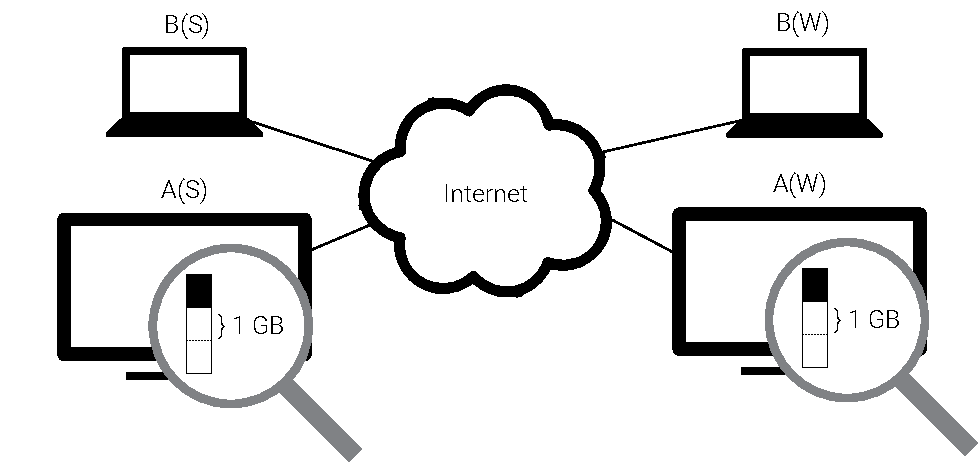
\includegraphics[]{images/partnerschaften_1.pdf}
	\label{partnerschaften_1}
  \caption{Wahl eines Geräts, auf dem Speicherplatz freigegeben wird.}
\end{figure}
Nun tauschen die Geräte A(S) und A(W) ihre Adressen aus und tragen sie beim jeweils anderen
in die Liste der Partnergeräte ein.
\begin{figure}[htb]
	\centering
  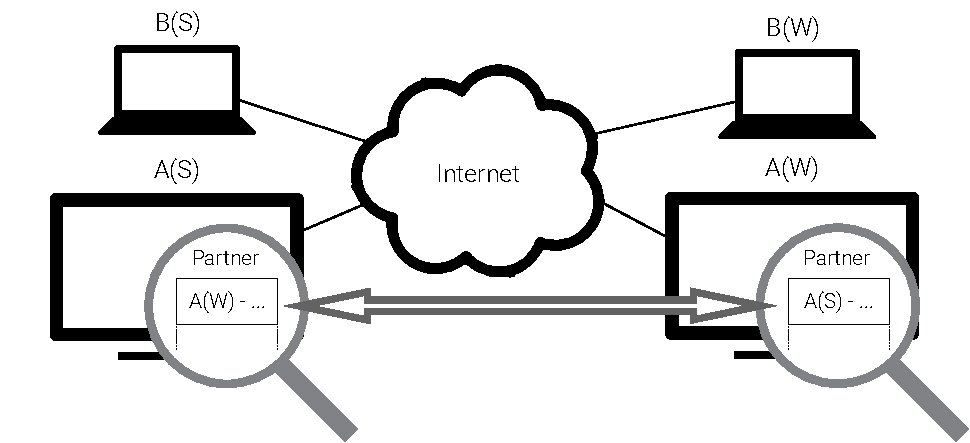
\includegraphics[]{images/partnerschaften_2.pdf}
	\label{partnerschaften_2}
  \caption{Austausch und Eintragen der Adressen.}
\end{figure}
Sobald beide Geräte gleichzeitig online sind, werden alle Geräte von Susanne auf Gerät A(W)
und umgekehrt alle Geräte von Wilfried auf Gerät A(S) gespeichert.
\begin{figure}[htb]
	\centering
  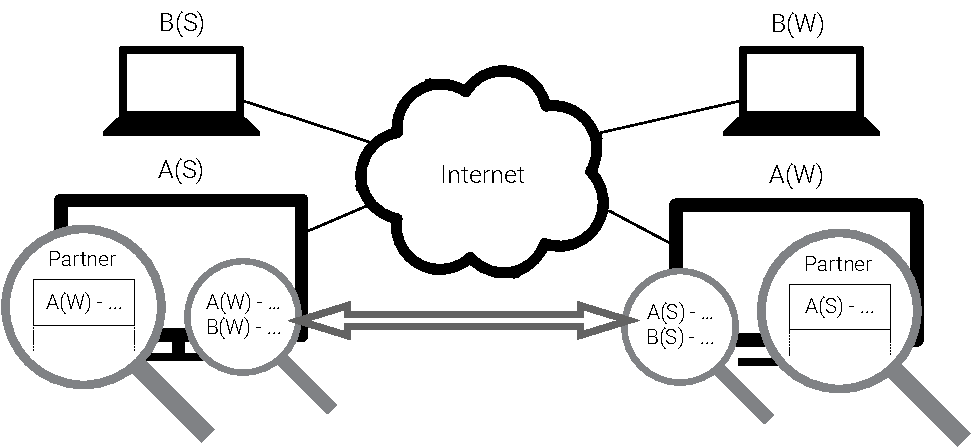
\includegraphics[]{images/partnerschaften_3.pdf}
	\label{partnerschaften_3}
  \caption{Eintragen der Geräte des Partners.}
\end{figure}
Weiters wird die Adresse von A(W) auf Susanne's Geräte und die Adresse von A(S) auf Wilfried's Geräte gespeichert.
\begin{figure}[htb]
	\centering
  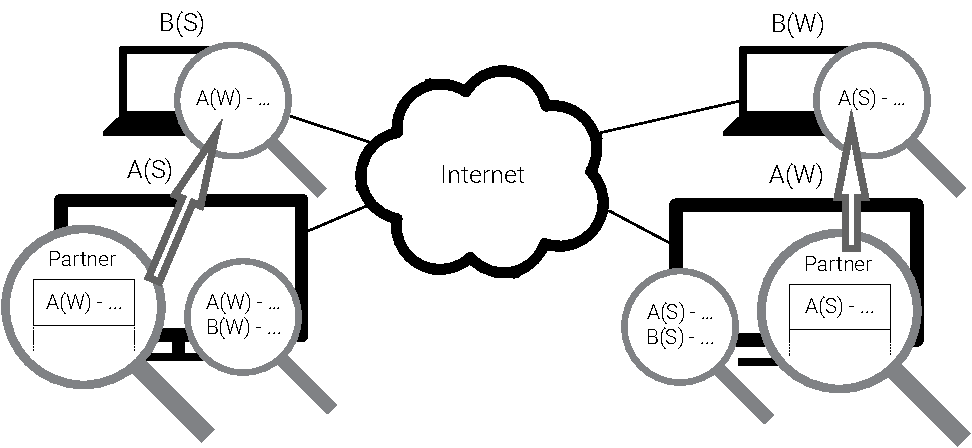
\includegraphics[]{images/partnerschaften_4.pdf}
	\label{partnerschaften_4}
  \caption{Eintragen der Adressen des Partnergeräts.}
\end{figure}
Ab diesem Zeitpunkt werden alle Änderungen von Susanne's Dateien auf Gerät A(W) gesichert,
bis sie auf alle Geräte von Susanne verteilt wurden. Sobald Susanne's Geräte die Änderung
erhalten, wird Gerät A(W) wieder aufgefordert, die Daten zu löschen. Das gleiche gilt natürlich
auch für Wilfried und das Gerät A(S).


\chapter{Graphical User Interface}\label{GUI}
\renewcommand{\kapitelautor}{Autor: Andreas Novak}

\section{Einleitung}
Mit dem Gedanken, dass ein Dateisynchronisationstool hauptsächlich im
Hintergrund arbeitet, ist die grafische Benutzeroberfläche zurückhaltend und
einfach gestaltet. Dem Nutzer werden nicht unnötig viel
Konfigurationsmöglichkeiten gegeben, damit er leicht den Überblick behalten
kann. Beim Starten von sblit erscheint das Icon im System-Tray, welches als
Angelpunkt für jegliche Nutzerinteraktion dient.

\section{System-Tray}\label{Systemtray}
\begin{figure}[H]
	\centering
	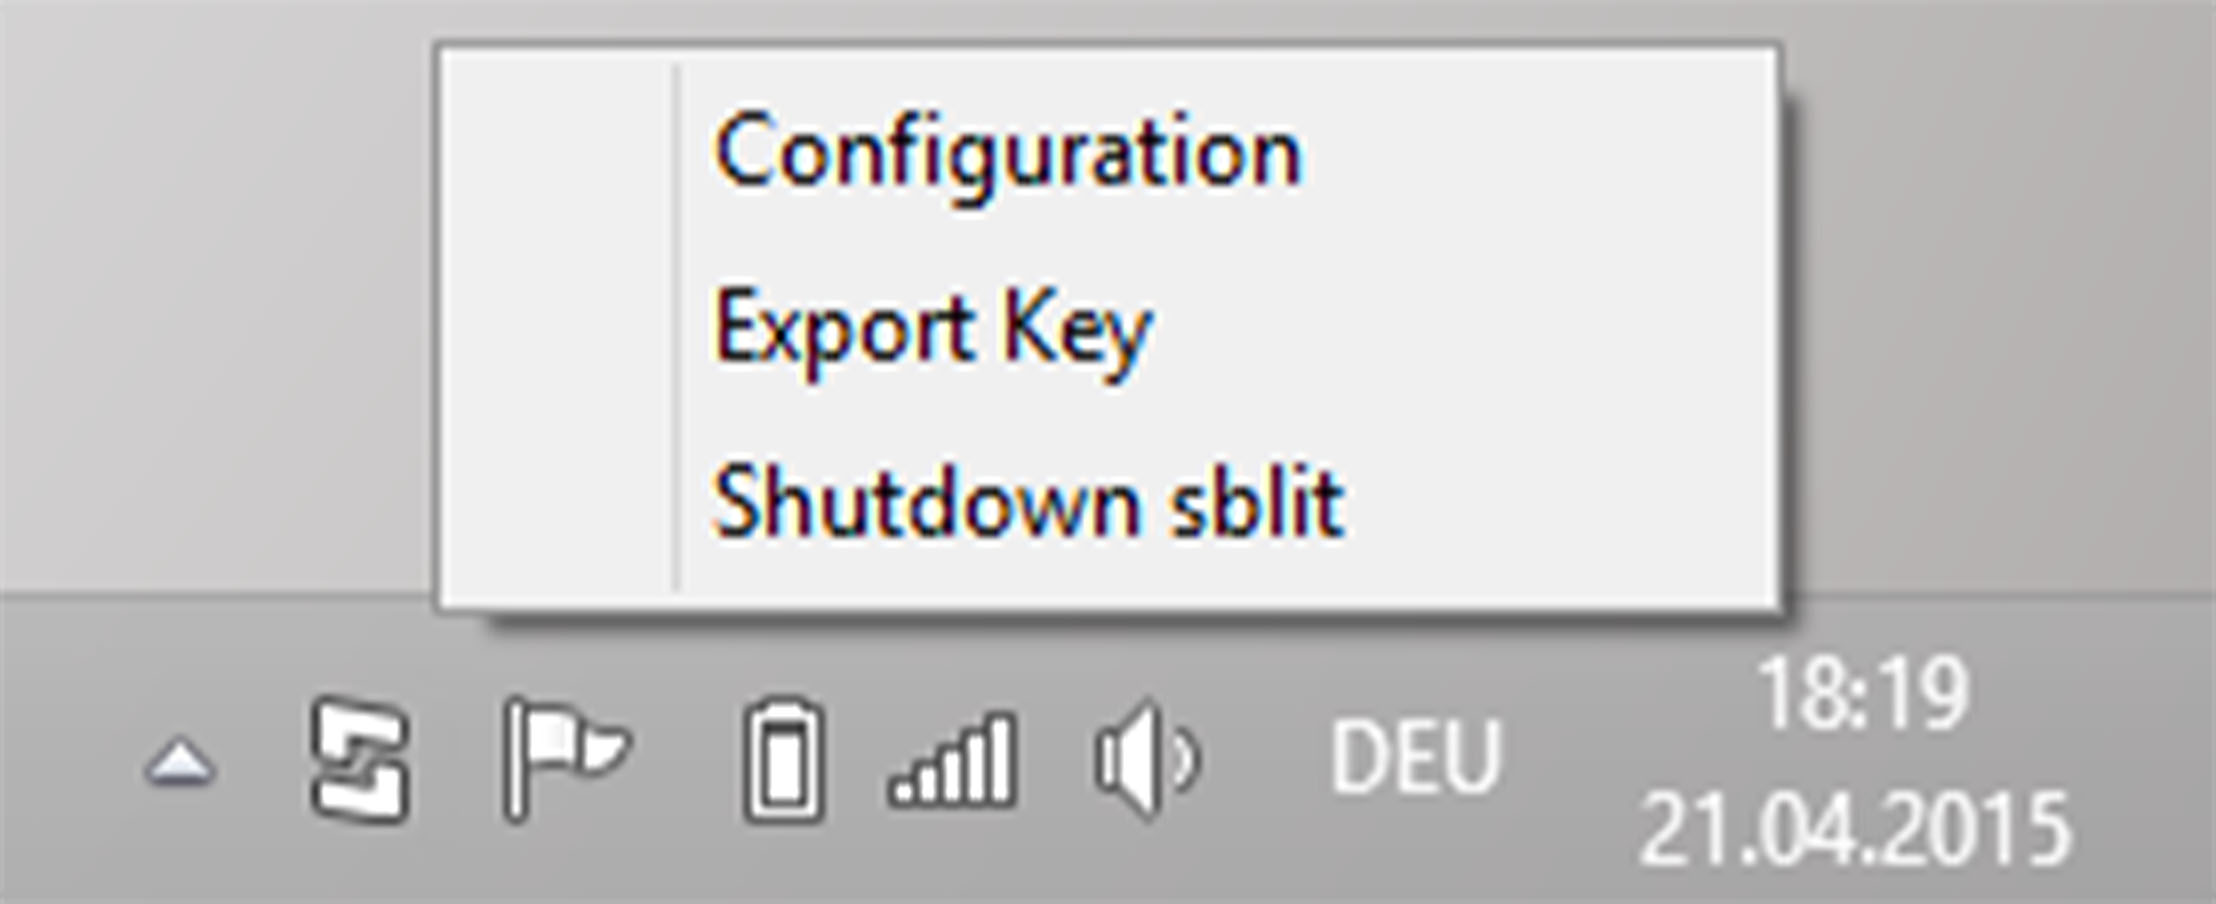
\includegraphics[]{images/systemtray.jpg}
  \caption{Menüfenster beim Systemtray}
\end{figure}

Mit einem Rechtsklick auf das Icon im System-Tray öffnet sich eine kleine Menüauswahl,
bei der folgende Punkte zur Auswahl stehen:

\begin{description}

	\descriptionitem{Configuration}
		Öffnet das Konfigurationsmenü.

	\descriptionitem{Export Key}
		Öffnet einen Dialog zur Auswahl des Speicherorts. In der exportieren Text-Datei befindet
		sich der öffentliche Schlüssel des eigenen Gerätes und der symmetrische Schlüssel für
		alle \gls{syncpartner}.

	\descriptionitem{Shutdown sblit}
	  Stoppt alle laufenden Synchronisationen und beendet die Anwendung.
\end{description}


\section{Überblicksfenster}\label{Überblicksfenster}
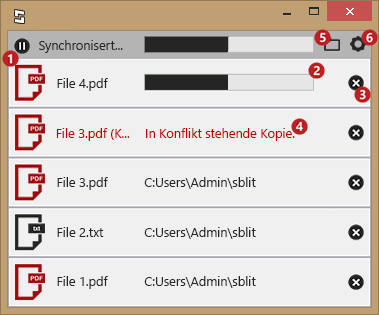
\includegraphics[]{images/systemtray.png}

Mit einem einfachen Klick auf das Icon öffnet sich die Übersicht, in der der
Benutzer auf die folgenden Optionen Zugriff bekommt:

\begin{description}

	\item[{Letzte Änderungen innerhalb des sblit-Ordners}]
		Dem Benutzer wird hier eine Auflistung der zuletzt hinzugefügten Dateien
		geboten. Neben dem an den Dateityp angepassten Bild, wird auch der Dateiname
		und Ordnerpfad angegeben.

	\item[{Fortschrittsbalken laufender Synchronisationsvorgänge}]
		Bei laufenden Synchronisationen hat der User die Möglichkeit, den
		Fortschritt zu verfolgen.

	\item[{Button für das Abbrechen der Synchronisation}]
		Bei irrtümlichem Hinzufügen von Dateien oder Ähnlichem, hat der Benutzer die
		 Möglichkeit, die laufende Synchronisation mithilfe des Löschen-Buttons
		abzubrechen.

	\item[{Anzeige von aufgetretenen Fehlern}]
		Bei Versionskonflikten, die auftreten, wenn 2 Synchronisationspartner die
		selbe Datei gleichzeitig bearbeiten, sowie bei diversen anderen Fehlern,
		wird der User benachrichtigt.

	\item[{Link zum sblit-Ordner}]
		Um dem Benutzer schnellen Zugriff auf seinen konfigurierten sblit-Ordner zu
		gestatten, gibt es den Ordner-Button, mit dem sich der sblit-Ordner im
		Datei-Browser öffnet.

	\item[{Öffnen des Konfigurationsmenüs}]
		Mit einem Klick auf den Optionen-Button öffnet sich das Konfigurationsmenü.
\end{description}


\section{Konfigurationsmenü}\label{Konfigurationsmenü}
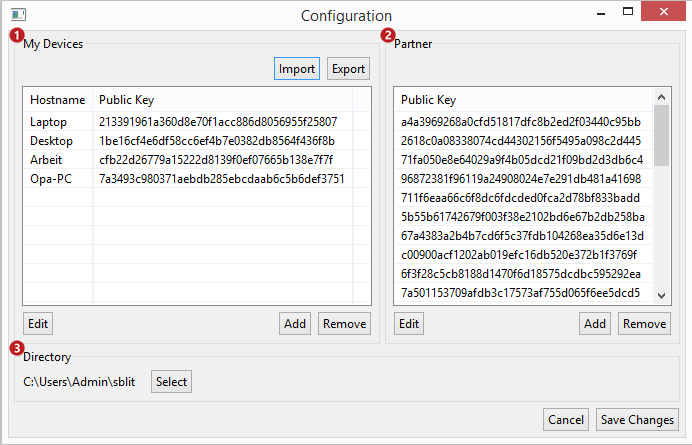
\includegraphics[]{images/config_gui.png}

\begin{description}

	\item[{Geräte zu den Synchronisationspartnern hinzufügen/entfernen}]
		Unter dem Punkt “My Devices” befindet sich die Liste der
		Synchronisationsgeräte, also jene Geräte, mit denen der unter Punkt 3
		angegebene sblit-Ordner synchronisiert wird. Die Einträge
		bestehen aus dem vom Benutzer angegebenen Namen des Geräts und dessen
		Public-Key, welcher seine Adresse darstellt.Der Benutzer hat die
		Möglichkeit, bestehende Einträge für Korrekturen zu bearbeiten, neue
		hinzuzufügen oder alte zu entfernen. Mit der Import- beziehungsweise der
		Export-Funktion der Liste, soll dem User das Übertragen der Liste auf neue
		Geräte erleichtert werden.

	\item[{Manuelles Eintragen von Partnergeräten}]
		Obwohl die Liste der Partnergeräte automatisch vom Programm verwaltet wird,
		hat der Benutzer die Möglichkeit, Geräte manuell hinzuzufügen. Während
		nämlich normalerweise Geräte fremder Nutzer als Partnergeräte fungieren,
		kann man sich auch gegenseitig mit einer Freundin oder einem Freund
		Speicherplatz freigeben, indem man den Public-Key des jeweils anderen in der
		Liste der Partnergeräte einträgt.

	\item[{Verschieben des sblit-Ordners}]
		Der zu synchronisierende Ordner kann im Konfigurationsmenü auch nach der
		Installation noch geändert und verschoben werden.

\end{description}


\chapter{Website}
\section{Allgemein}
Zu Beginn des Projektes war es Bestandteil der Diplomarbeit eine Website als
Onlinepräsenz zu gestalten, auf der die Projektidee, die Teammitglieder und der
Projektstatus einsehbar sind.

Primär lag aber die Applikation im Fokus unserer Diplomarbeit, weshalb wir uns
an Bootstrap bedient haben, einem offenen CSS-Framework, das viele vordefinierte
Auszeichnungen für HTML-Elemente aller Art bietet.

Viele Frontend-Entwickler veröffentlichen ihre eigenen Bootstrap-Themen, also
mit bootstrap-Klassen desginte, statische HTML-Seiten und machen es Anwendern
möglich, diese bestehenden Frontend-Webseiten für eigene Zwecke umzugestalten
und schnell für einen schönen und einfachen Web-Auftritt zu sorgen. Namenhafte
Webseiten, auf denen verschiedenste Bootstrap-Themen ausgestellt und unter
anderem zur Verwendung frei gestellt sind wären \href{http://startbootstrap.com/}{startbootstrap.com},
\href{http://bootstrapzero.com/}{bootstrapzero.com} oder \href{http://blacktie.co/}{blacktie.co}.

Der Webauftritt der Diplomarbeit ist aus solch einem Bootstrap-Thema von
startbootstrap.com entstanden, welches optisch und inhaltsmäßig auf unsere
Diplomarbeit angepasst worden ist. Dabei wurde ein, für Bootstrap typisches
One-Page-Design verwendet.

\section{Screenshot}
% TODO: Website-Screenshot miteinbinden.
% + Websiten zu Hyperlinks machen

\chapter{Wettbewerbe}
\renewcommand{\kapitelautor}{Autor: Andreas Novak}

\section{Allgemein}
Jedes Jahr gibt es für Studierende, Schülerinnen und Schüler die Möglichkeit, ihre privaten
oder die ihm Rahmen ihrer Ausbildung entstandenen Projekte bei Projekt-Wettbewerben
einzureichen. Für Diplomarbeiten wie \sblit stellen diese Wettbewerbe eine einfache und effektive
Methode dar, um Marketing zu betreiben und den Bekanntheitsgrad des Projekts zu steigern.

Mit einem Projekt, das eine kreative Idee besitzt, aktuelle Themen behandelt und technischen Tiefgang hat,
finden sich leicht Interessenten unter den zahlreichen Besuchern von Projektwettbewerben.

Durch die Schule wurden die Mitglieder aller Diplomarbeiten über diverse Vertreter
solcher Wettbewerbe informiert. Das \sblit-Diplomarbeitsteam hat das Projekt daraufhin bei einigen
Wettbewerben eingereicht. Der folgende Abschnitt behandelt die Wettbewerbe, bei denen das Projekt
eingereicht wurde und die dafür erforderlichen Dokumente.

\section{Wettbewerbe}
\subsection{Jugend Innovativ}
\subsubsection{Allgemein}
Jugend Innovativ ist der größte Wettbewerb für innovative Schulprojekte in Österreich und
bietet Jugendlichen die Möglichkeit, ihre innovativen Projekte von einer Fachjury bewerten zu lassen
und mit etwas Glück unter den Gewinnern zu landen, denen ein Preisgeld von bis zu 2000€ zugesprochen wird.

\subsubsection{Einreichung}
Nachdem \sblit in der Kategorie idea.goes.app eingereicht wurde, musste für den Wettbewerb ein
Projektstatusbericht verfasst werden, der einen einen genauen Einblick in das Projekt geben soll
und zusätzlich auch die Ergebnisse aufzeigt, die bis dato erzielt wurden.

\subsubsection{Ergebnis}
Vorerst (Stand April 2015) sind nur die Halbfinalisten der teilnehmenden Projekten bekannt.
Aus diesem Grund wurde das Diplomarbeitsteam
zum gleichnamigen Halbfinal-Event eingeladen, um das Projekt vorort auszustellen.

Um den eigenen Projektstand zu schmücken wurde ein Plakat angefertigt, auf dem die Eckdaten unseres
Projekts einsehbar sind.
Zusätzlich wurden zum erleichterten Weiterreichen der Kontaktinformationen des Projektteams Visitenkarten
entworfen und gedruckt. Einsehbar sind diese im Anhang auf der \pagelink{visitenkarte}.

\subsection{u19 -- Create your World}
\subsubsection{Allgemein}
u19 – CREATE YOUR WORLD ist der Jugendwettbewerb des Prix Ars Electronica, einem der traditionsreichsten Medienkunstwettbewerbe Österreichs.
Hier wird die Möglichkeit geboten, eigene Vorstellungen und Ideen zu realisieren und zu präsentieren.

\subsubsection{Einreichung}
Ursprünglich wurde das Projekt selbst als Dateiabgabe oder eine technische Dokumentation als Abgabe gefordert. Da \sblit zu diesem Zeitpunkt
aber noch nicht fertiggestellt wurde und auch nicht als einzelne Datei abgegeben hätte werden können,
einigte man sich mit den Organisatoren darauf, einen Projektfolder einzureichen, der die Projektidee
beschreibt und noch nähere technische Details zu den einzelnen Teilgebieten und den Projektstatus beinhaltet. Einsehbar ist diser im Anhang auf der \pagelink{projectfolder}.


\subsubsection{Ergebnis}
Die Ergebnisse wurden noch nicht bekanntgegeben (Stand April 2015).

\subsection{AXAWARD}
\subsubsection{Allgemein}
AXAWARD steht für AUSTRIAN X.TEST AWARD und ist ein Wettbewerb für technische Schulprojekte und Forschungsarbeiten
von Teams mit bis zu 3 Mitgliedern und wird von der österreichischen Messtechnik-Firma x.test veranstaltet.

\subsubsection{Einreichung}
Auch beim AXAWARD wurde das Projekt selbst als Dateiabgabe oder eine technische
Dokumentation als Abgabe gefordert. Aufgrund dessen wurde auch bei diesem Wettbewerb der Projektfolder eingereicht. Dieser ist im Anhang auf der \pagelink{projectfolder} einsehbar.

\subsubsection{Ergebnis}
Die Finalteams des AXAWARD 2015 wurden im April 2015 per Mail bekanntgegeben, wobei es \sblit nicht
unter die besten zehn Projekte geschafft hat. Genauere Platzierungen wurden nicht bekannt gegeben.


\subsection{Internet of Things Cup}
\subsubsection{Allgemein}
Der Internet of Things Cup ist ein Open Source Projektwettbewerb für Studierende, Schülerinnen und Schüler,
der den Fokus auf das namensgebende Internet der Dinge legt. sblit eignet sich insofern für den Wettbewerb,
als dass, basierend auf einzelnen Komponenten der Umsetzung, dezentrale Speicher- und Kommunikationsmöglichkeiten
geschaffen werden können, die in Internet of Things und Machine-to-Machine-Anwendungen integriert werden können.

Für das Projekt wurde dem Diplomarbeitsteam kostenlose Hard- und Software zur Verfügung gestellt: ein
Beaglebone-Mikrocomputers, eine Jahreslizenz für Microsofts Azure Datenbank und Conrad Gutscheine.

\subsubsection{Einreichung}
Im April war die Abgabe des Projekt-Zwischenberichts, welcher die erste Abgabe nach
der Einreichung darstellt. Der Bericht setzt sich aus einem Google-Drive-Fragebogen
zusammen, bei dem grundsätzliche Informationen an die Wettbewerbsleitung übergeben
werden, wie zum Beispiel der Projektstatus in Prozentangabe oder auch das Beilegen
von Grafiken des Projekts. Zudem waren noch relevante Links wie zum Beispiel zu der
Projekt-Website oder Social-Media-Seiten anzugeben.

\subsubsection{Ergebnis}
Ergebnisse wurden noch nicht bekanntgegeben, da dieser Wettbewerb noch am Laufen ist.
Die Siegerehrung des IoT Cups findet am 3. Juli 2015 statt.

\subsection{Computer Creative Wettbewerb}
\subsubsection{Allgemein}
Beim Computer Creative Wettbewerb, der von der Oesterreichischen Computer Gesellschaft
organisiert wird, ist die Ausarbeitung eines Projekts, das sich kreativ mit Informatik
auseinandersetzt, das Ziel. Die Bewerber dürfen dabei nur jünger als 21 Jahre sein.

Die eingereichten Projekte kommen aus verschiedensten Teilbereichen der Informatik,
sodass sich diverse Arbeiten mit Multimedia, Internet, Robotik, Webseitengestaltung, Spielen oder
Programmieren als Thematik gegenüberstehen und miteinander verglichen werden.

Für die ersten fünf in jeder Kategorie gibt es Geldpreise zu gewinnen.

\subsubsection{Einreichung}
\sblit zählt zur Sekundarstufe II, also Oberstufe von 14 bis 20 Jahren. Zur Teilnahme
musste ein Online-Formular ausgefüllt und eine detaillierte Projektbeschreibung
verfasst und abgegeben werden. Auch bei diesem Wettbewerb wurde der Projektfolder
abgegeben, welcher im Anhang auf der \pagelink{projectfolder} einsehbar ist.

\subsubsection{Ergebnis}
Einsendeschluss der Projekte war bis April, weshalb dieser Wettbewerb noch einige Zeit
andauern wird. Genauere Termine sind noch nicht bekannt.




%%%%%%%%%%%%%%%%%%%%%%%%%%%%%%%%%%%%%%%%%%%%%%%%%%%%%%%%%%%%%%%%%%%%%%%%%%%%%%%%%%%%%%%%%%
% wer hat diese Kapitel geschrieben oder leer
\renewcommand{\kapitelautor}{}

\appendix


\chapter{Anhang 1\label{appendix1}}

% inkludiertes PDF auf der rechten Seite beginnen:
\cleardoublepage
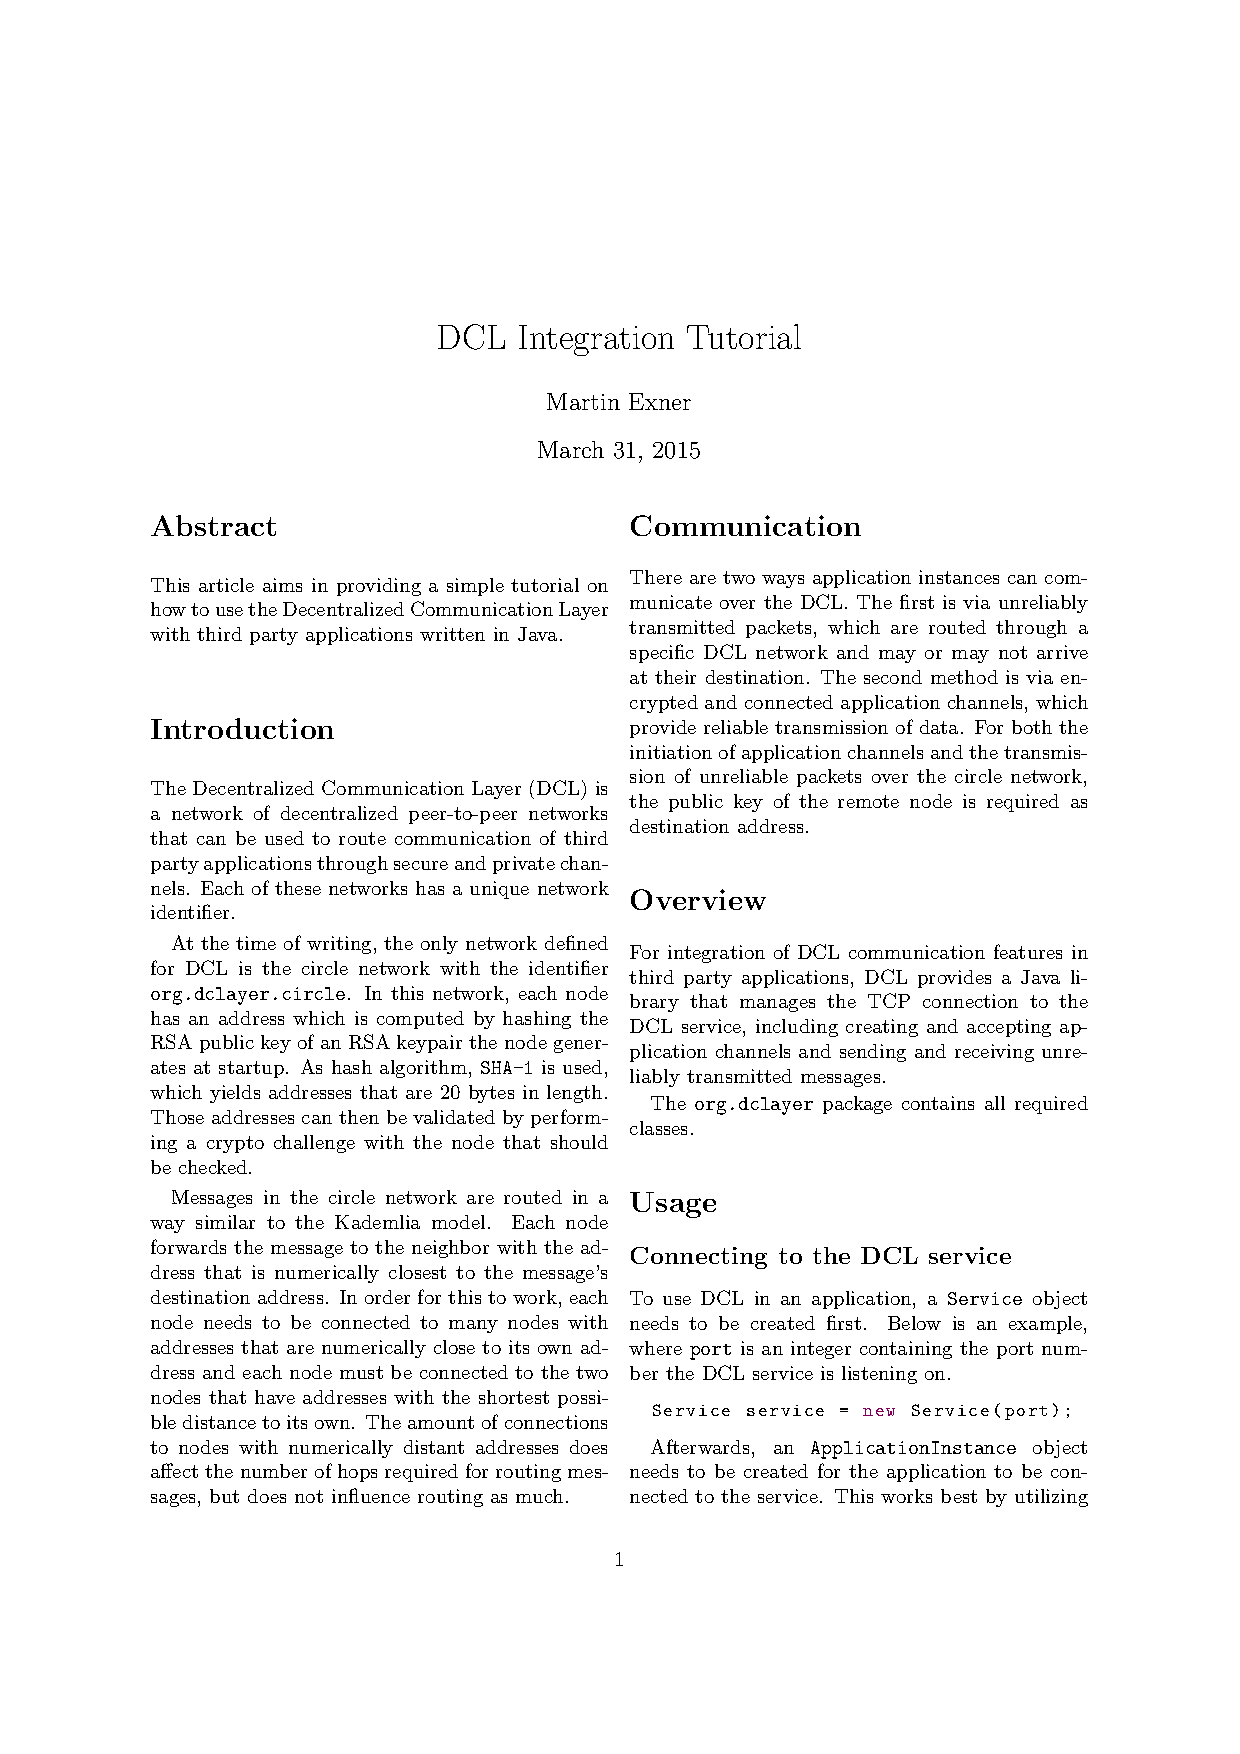
\includepdf[pages=-,width=210mm,height=297mm]{../dcl_tutorial/dcl_tutorial.pdf}

\chapter{Anhang 2\label{appendix2}}

\cleardoublepage

\includepdf[pages=-,width=210mm,height=297mm]{../wettbewerbe/flyer.pdf}

\chapter{Anhang 3\label{appendix3}}
\begin{figure}[htb]
	\centering
	
\includegraphics[width=85mm,height=55mm]{images/visitenkarte_vorderseite.pdf}
	\label{visitenkarte_vorderseite}
  \caption{Vorderseite der Visitenkarte}
\end{figure}

\begin{figure}[htb]
  	\centering
  	
\includegraphics[width=85mm,height=55mm]{images/visitenkarte_rueckseite.pdf}
  	\label{visitenkarte_rueckseite}
    \caption{Rückseite der Visitenkarte}
\end{figure}

\printindex{}

\bibliographystyle{plaindin}
\bibliography{diplom}

\printglossary[type=\acronymtype]
\printglossary

\end{document}
